%-----------------------------------------------------------------------------
%	PACKAGES AND DOCUMENT CONFIGURATION
%-----------------------------------------------------------------------------

% Use `report` class with `USCthesis` package (style file) by Brian P. Gerkey
\documentclass[11pt]{report}
% [options] can be any of these default/alternative flag:
%   dissertation/thesis, final/proposal, copyright/nocopyright,
%   fussy/sloppy, flushbottom/raggedbottom, clref/opref.
\usepackage[dissertation]{USCthesis}

% Packages required by `USCthesis.sty`.
\usepackage{setspace}
\usepackage{tabularx}
% Filler text for formatting. Comment these lines out for real writing.
\usepackage[english]{babel}
\usepackage{blindtext}

%%% asif's packages
\usepackage{amsmath}
\usepackage{graphicx}
\usepackage[colorinlistoftodos]{todonotes}
\usepackage{hyperref}
\usepackage{float}
\usepackage{verbatim}
\usepackage{color,soul}
%\usepackage{caption}

\begin{document}

%-----------------------------------------------------------------------------
%	TITLE PAGE
%-----------------------------------------------------------------------------

% Volume name could be added as option, e.g. `[Volume I]`.
\title{Bayesian Analysis of Transcriptomic and Genomic Data}

\author{Asif Zubair}

% Committee list is only shown in `proposal` layout.
\committee{A.~Adams & (Chair)\\*
           B.~Bell\\*
           C.~Clausius\\*
           D.~Dirichlet\\*
           E.~Emory & (Outside Member)}

% Submission information is only shown in `final` layout.
\majorfield{Computational Biology and Bioinformatics}
\submitdate{May 2019}

%-----------------------------------------------------------------------------
%	PREFACE
%-----------------------------------------------------------------------------

% The preface environment prints the title page.


\begin{preface}
%\captionsetup{font={large,stretch=3.3}}

  % Dedication Page, which is truly unnecessary.
  \prefacesection{Dedication}
     \begin{quote}
         \raggedleft {\em To my closest ancestors}\\
         \raggedleft {\em and full-sibs.}
     \end{quote}


  % Acknowledgement Page, which is also unnecessary for proposals.
  \prefacesection{Acknowledgements}
    % Better to separate LaTeX structure and content
    I am greatly indebted to my advisors, Profs. Paul Marjoram and Sergey Nuzhdin, and my committee member, Prof. Gary Rosen, for their continued support, intellectual stimulation and encouragement. Their guidance and support has helped me to explore diverse topics and experience a great breadth of research during my studies. I, also, benefited greatly from their wisdom and their mentorship will continue to have a profound effect on me throughout my life. 

I would also like to thank all my collaborators who I had the great privilege of working with during my research. They come from diverse cultural and intellectual backgrounds and each interaction has greatly enriched me. 

I would like to thank the funding agencies that supported my work and would like to thank the graduate school for supporting me through the Provost fellowship. 

  \tableofcontents
  \begin{comment}

  \listoftables
  \listoffigures

  % Abstract Page
  \prefacesection{Abstract}
    Bayesian methods offer a way of doing a fully probabilistic analysis for inference problems and for dealing with uncertainty. 
They offer a number of advantages over more conventional statistical techniques and have become widely used in the fields of genetics, genomics, bioinformatics and computational systems biology, in an effort to make sense of complex noisy data. 
Here, we describe an application area dealing with modeling spatial patterning in developing \textit{Drosophila} embryo.
In addition, after describing an analysis of association mapping in chickpea hybrids, we provide a perspective on how to integrate quantitative biology and systems biology approaches to increase power in association mapping studies.
Finally, I take a digression to describe a study on transposable element expression and chromatin accessibility in human cancer cells. 

    \end{comment}
\end{preface}

%-----------------------------------------------------------------------------
%	CONTENT STRUCTURE
%-----------------------------------------------------------------------------

% Better to separate LaTeX structure and content
\chapter{Introduction \& Overview}
\label{cha:introduction}

%This chapter talks about motivation and applications of my work, and reviews previous research in the field.

%\section{Motivations}
%\label{sec:motivations}

%Previous research\cite{Fisher:1954} \cite{Robbins:1951aa} \cite{Knight:1921} in the field of X has established that method A is very useful.
%Another branch of researchers\cite{Wright:1921aa} \cite{Caratheodory:1909aa} \cite{Gibbs:1902} \cite{Clausius:1857} have figured out that method B could be better in certain occasions.
%Here I propose a new method that gives results better than both types.

Here I present a brief overview of the chapters in the dissertation. 


%embryo
In chapter \ref{cha:research_topic_1}, I address the problem of spatial pattering in \emph{Drosophila} embryos, specifically the gap gene system. The gap gene system controls the early cascade of the segmentation pathway in Drosophila melanogaster as well as other insects. Owing to its tractability and key role in embryo patterning, this system has been the focus for both computational modelers and experimentalists. The gap gene expression dynamics can be considered strictly as a one-dimensional process and modeled as a system of reaction-diffusion equations. While substantial progress has been made in modeling this phenomenon, there still remains a deficit of approaches to evaluate competing hypotheses. Most of the model development has happened in isolation and there has been little attempt to compare candidate models.

The Bayesian framework offers a means of doing formal model evaluation. Here, we demonstrate how this framework can be used to compare different models of gene expression. We focus on the Papatsenko-Levine formalism, which exploits a fractional occupancy based approach to incorporate activation of the gap genes by the maternal genes and cross-regulation by the gap genes themselves. The Bayesian approach provides insight about relationship between system parameters. In the regulatory pathway of segmentation, the parameters for number of binding sites and binding affinity have a negative correlation. The model selection analysis supports a stronger binding affinity for Bicoid compared to other regulatory edges, as shown by a larger posterior mean. The procedure doesn’t show support for activation of Kruppel by Bicoid.
We provide an efficient solver for the general representation of the Papatsenko-Levine model. We also demonstrate the utility of Bayes factor for evaluating candidate models for spatial pattering models. In addition, by using the parallel tempering sampler, the convergence of Markov chains can be remarkably improved and robust estimates of Bayes factors obtained.

%chickpea
Chapter \ref{cha:research_topic_2} introduces nested association mapping (NAM) populations for chickpea hybrids. NAM populations utilize the framework of common reference design to produce synthetic
mapping populations that take advantage of both historic and recent recombination events such
that marker density requirement is kept low while having higher allelic richness and statistical
power. Pursuant of this aim, and keeping in mind that our goal is to introgress favourable alleles
from wild populations into cultivated varieties, crosses of wild chickpea species, C. reticulatum, called wild founders, were made with three different elite cultivars.

In the present analysis, we examine hybrid crosses of wild founders with the elite cultivar,
ICCV96029. Limiting ourselves to species divergent markers, we conduct an association study
with six continuous phenotypes including important traits like yield and shattering index. This
reveals important features of the genomic architecture underlying these traits. 

Having provided an introduction to the Bayesian framework and an analysis for association mapping in chickpea hybrids, chapter \ref{cha:research_topic_3} provides a perspective on how the Bayesian approach can be used to improve association mapping. The power of genome-wide association studies (GWAS) rests on several foundations: (i) there is a significant amount of additive genetic variation, (ii) individual causal polymorphisms often have sizable effects and (iii) they segregate at moderate-to- intermediate frequencies, or will be effectively ‘tagged’ by polymorphisms that do. Each of these assumptions has recently been questioned. (i) Why should genetic variation appear additive given that the underlying molecular networks are highly nonlinear? (ii) A new generation of relatedness-based analyses directs us back to the nearly infinitesimal model for effect sizes that quantitative genetics was long based upon. (iii) Larger effect causal polymorphisms are often low frequency, as selection might lead us to expect. 

In chapter \ref{cha:research_topic_3}, we review these issues and other findings that appear to question many of the foundations of the optimism GWAS prompted. We then present a roadmap emerging as one possible future for quantitative genetics. We argue that in future GWAS should move beyond purely statistical grounds. One promising approach is to build upon the combination of population genetic models and molecular biological knowledge. This combined treatment, however, requires fitting experimental data to models that are very complex, as well as accurate capturing of the uncertainty of resulting inference. This problem can be resolved through Bayesian analysis and tools such as approximate Bayesian computational method growing in popularity in population genetic analysis. We show a case example of anterior-posterior segmentation in Drosophila, and argue that similar approaches will be helpful as a GWAS augmentation, in human and agricultural research.

Finally, in chapter \ref{cha:research_topic_4}, I discuss an important analysis on transposable elements (TEs) and their implication in cancer progression and relapse. Genomic transposable elements comprise nearly half of the human genome. The expression of TEs is considered potentially hazardous, as it can lead to insertional mutagenesis and genomic instability. However, recent studies have revealed that TEs are involved in immune-mediated cell clearance. 

Hypomethylating agents can increase the expression of TEs in cancer cells, inducing `viral mimicry', causing interferon signalling and cancer cell killing. To investigate the role of TEs in the pathogenesis of acute myeloid leukaemia (AML), we studied TE expression in several cell fractions of AML while tracking its development (pre-leukemic haematopoietic stem cells, leukemic stem cells (LSCs), and leukemic blasts) and chromatin accessibility in these cells. 

LSCs, which are resistant to chemotherapy and serve as reservoirs for relapse, showed significant suppression of TEs and interferon pathways. We propose TE suppression as a mechanism for immune escape in AML. Repression of TEs co-occurred with the upregulation of several genes known to modulate TE expression, such as RNA helicases and autophagy genes. Thus, we have identified potential pathways that can be targeted to activate cancer immunogenicity via TEs in AML.

All published work is indicated with a reference number in the title of the chapters. Additionally, in Appendix \ref{appendix}, I list side projects that I worked on and that have been published. 

% embryo
\chapter{Bayesian model selection for the \textit{Drosophila} gap gene system \cite{zubair2019}}
\label{cha:research_topic_1}

\section{Background}

The process by which multicellular organisms develop from a single fertilized cell has been the focus of much attention. It was postulated that organisms are patterned by gradients of certain form-producing substances. Boveri \cite{boveri1901} and Horstadius \cite{horstadius35} used this idea to explain the patterning of the sea urchin embryo. The idea was given further impetus by the discovery of the Spemann organizer \cite{spemann24} which suggested that morphogenesis is the result of signals released from localized group of cells. In 1952, Turing, working on the problem of spatial patterning, coined the term morphogen to describe `form-producers'. He used mathematical models to show that chemical substances could self-organize into patterns starting from homogeneous distributions \cite{turing52}. However, a definitive example of a morphogen was only provided in 1987 by the discovery of Bicoid function in the \textit{Drosophila} embryo \cite{nusslein80,nusslein87} and subsequent visualization of its gradient \cite{driever88a,driever88b}. Not surprisingly, patterning in the \textit{Drosophila} embryo has been the focus of both developmental and systems biologists. 

The formation of several broad gap gene \cite{jaeger11} expression patterns within the first two hours of development characterizes early \textit{Drosophila} embryogenesis. Taken together, the gap genes constitute one of the four regulatory layers in the cascade of segmentation pathway in \textit{Drosophila} embryo. Expression of gap genes is regulated by maternal genes \cite{hulskamp90} and they also participate in mutual repression \cite{kraut91}. Thus, activation  by maternal gradients, combined with spatially specific gap-gap cross repression helps to establish, sharpen and maintain the broad overlapping domains of the gap gene expression along the Anterior-Posterior (A-P) axis. The gap gene network is one of the few examples of a developmental gene network which has been studied extensively using data-driven mathematical models \cite{jaeger04b,jaeger09,jaeger12} in order to reconstruct the regulatory structure of the gap gene network. However, there continues to be active discussion \cite{papatsenko08,zinzen07} on how maternal gradients and mutual gap gene repression contribute to the formation of gap stripes. 

Mathematical representation of the gap gene network through quantitative dynamical systems has helped investigate regulatory structure of this network along with specific properties of this representation such as the strength of interaction, cooperativity of regulators, etc. However, there is a deficit of a rigorous framework within which putative representations can be compared and allows one to conduct formal statistics of relative fit. In a seminal paper, Jaeger \textit{et al.} \cite{jaeger04b} used a dynamical model where a genetic inter-connectivity matrix described the regulatory parameters. Based on measures of model fit, they argued that dual regulatory action of Hunchback on Kruppel is not essential for to explain gap gene domain formation. While this may be valid, they do not provide a relative goodness of fit of the model against a representation that assumes dual-regulation. Perkins et al. \cite{jaeger06b} did an extensive study of gap gene regulatory relationships and compared proposed networks in literature. However, their study does not provide a measure of statistical significance for model comparison. Essentially, the question we want to ask is how to chose between competing hypothesis for the network structure in a statistically rigorous manner ? In addition, real data is often contaminated with measurement noise and we need methods that can help us deal with this uncertainty. 

Addressing the latter point, one way to handle error associated with experimental observations is to model it as Gaussian noise. If we know or are willing to assume a model for the error variance, then an estimate of the parameters can be sought by maximizing the likelihood in a least squares sense. This is the maximum likelihood estimate (MLE) \cite{stigler07} of the parameters. However, this point estimate suffers from being unrepresentative and is often intractable, especially if the likelihood is multimodal. 
An alternative approach is the Bayesian framework which allows one to not only account for experimental error by propagating it to the model parameters but also a way to integrate our prior beliefs on the distribution of model parameters. In this manner, a posterior distribution of the model parameters is obtained which encapsulates our belief in the parameter values given uncertainty in measurement. Indeterminacy of model parameters and correlations between indeterminate parameters are incorporated into the marginal likelihood (evidence). Direct computations of integrals involved in Bayesian methods are difficult and so researchers tend to use Markov chain Monte Carlo (MCMC) methods like Gibbs sampling or Metropolis-Hastings algorithm \cite{hastings70}. Bayesian approaches have enjoyed great success in genetics \cite{beaumont04} and we and others \cite{wilkinson07} expect that they will provide more satisfactory solutions to inference problems in computational systems biology.

In addition, the Bayesian approach allows us to assess which of the competing models is better supported by the data by comparing the ratios of marginal likelihood of the models. The process of comparing models is more formally known as model selection and the ratio of marginal likelihoods is also called the Bayes factor \cite{raftery95}. It follows, that in order to use Bayes factors, one needs to estimate the marginal likelihood of a model.  However, this task becomes increasingly intractable with growing model dimensionality and a conventional Metropolis-Hastings sampling approach generally leads to poor mixing properties and unreliable conclusions. To overcome this difficulty, we use the parallel tempering Markov chain Monte Carlo (PT-MCMC) sampling technique \cite{geyer91}. Briefly, this method runs parallel chains at different temperatures (or degree of smoothness of likelihood surface) and allows exchanges between the chains based on the Hastings ratio. The end result is a chain that mixes well and also doesn’t get stuck in local optima. Another benefit of this approach is that it allows one to use path integration to compute the thermodynamic estimator \cite{meng98} of the marginal likelihood. This estimator has been shown to be reliable when working with Bayes factors \cite{calderhead10} in the context of differential equations. 

We currently focus on the Papatsenko-Levine formalism \cite{papatsenko11}, which exploits a fractional occupancy based approach to incorporate activation of the gap genes by the maternal genes and cross-regulation by the gap genes themselves. An advantage of this formalism is that it incorporates non-linear effects between regulatory interactions and is closer to a mechanistic view of how regulation in this system occurs \cite{jaeger06a}. While in their paper, Papatsenko \& Levine assumed that network structure is known \textit{a priori}, our approach allows one to choose from competing network topologies reported in the literature and to vary strength of interactions between gap genes. It is worth mentioning here that although we consider models of increasing complexity, Bayes factors allows model comparison without concerns of over-fitting, that is, they allow one to implicitly control for model dimensionality \cite{jeffreys92}.	

\section{Methods}

\subsection{Expression Data}

We use published data by Papatsenko \& Levine \cite{papatsenko11}. This data was obtained from the FlyEx database \cite{pisarev09}. The data comprise of expression values on a line along the Anterior-Posterior axis of the embryo and subsampled to 100 spatial points separated by approximately $5\mu m$. Maternal Bicoid (Bcd) and Hunchback (Hb) expression data corresponding to cleavage cycle 14.1 were used as input to the model. The output data is gap gene zygotic expression at cleavage cycle 14.4 for Hunchback, Kruppel (Kr), Knirps (Kni) and Giant (Gt) (fig. 1). Tailless (Tll) expression data corresponding to cleavage cycle 14.4 was also used as input. 

\begin{figure}
    \centering
    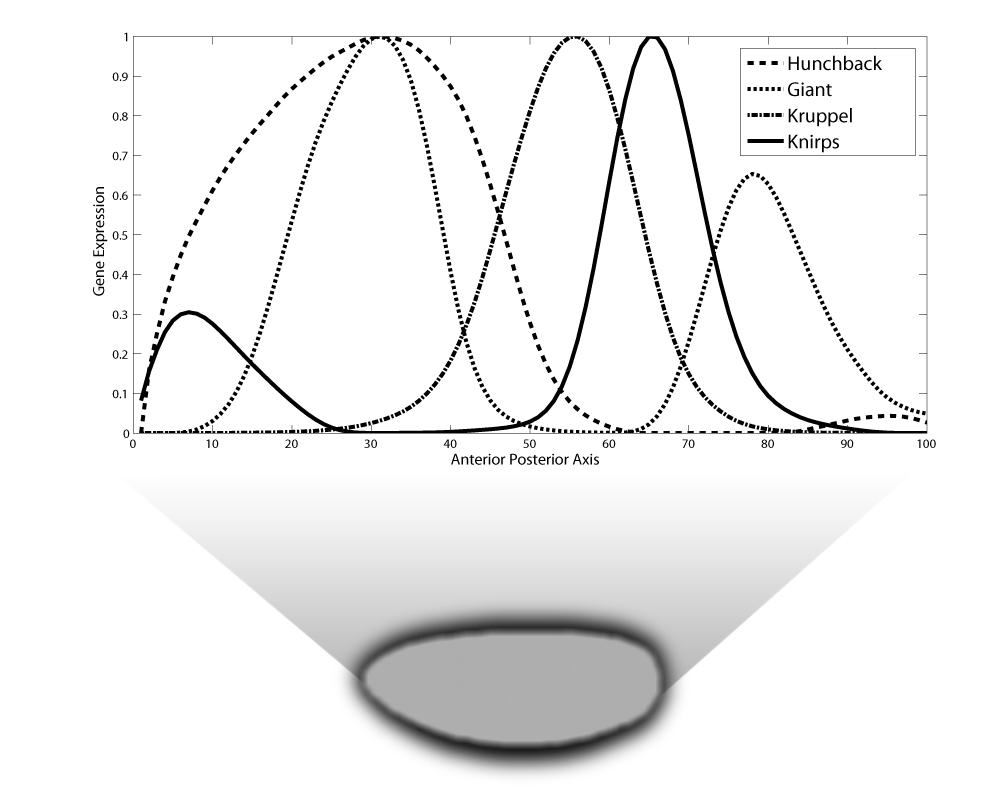
\includegraphics[scale = 3.0]{tex/embryo/figure-1.jpg}
    \caption{Expression data: Gap gene expression values at cleavage cycle 14.4 along the anterior-posterior axis of developing embryo are used to fit the model.}
    \label{fig:figure-1}
\end{figure}

\subsection{Models}

Time-varying systems can be modeled with ordinary differential equations (ODEs) which have efficient solvers available (for example, \cite{hindmarsh05}) . However, in pattern formation gene expression varies both in time and space and partial differential equations (PDEs) are the suitable method for characterizing this process. Closed form solutions for PDEs exist only in the most simplest of cases and numerical solutions need to be employed. Packaged solvers for PDEs do exist \cite{GWAT:GWAT584} and some like deal.II \cite{Bangerth2007} have been used in systems biology applications \cite{garikipati2017, murphy2018, albert2014}. However, due to the overhead of generalizability and computational tractability in structuring models, we wrote our own solver.

We first elaborate the PDE formalism, due to Papatsenko \& Levine, used for describing gap gene expression:

\begin{align*}
	\frac{\partial }{\partial t}u_{i}(x,t) &= \alpha P_{i}^{A}(1 - P_{i}^{B}) - \beta u_{i}(x,t) + D \frac{\partial^2 u_{i}(x,t)}{\partial x^2}, \\
	i &= Hb, Kr, Kni, Gt, \\
	u'(0,t) &= u'(L,t) = 0, u' = \frac{\partial u}{\partial x}, \\
	0 &< x < L, 0 < t < T.
\end{align*}

Here, $u_{i}(x,t)$ represents the expression of gap gene, $i$, at time $t$ and position $x$ with Neumann boundary conditions, i.e., we assume that flux at the boundaries is zero.  $\alpha$ represents the production rate, $\beta$ is the linear decay rate and $D$ is the diffusion constant. $L$ denotes the length of the embryo and $T$ corresponds to cleavage cycle 14.4 which marks the start of gastrulation. $P^A$ and $P^B$ are respectively combined activation and repression effects of regulators for each gap gene. These regulatory effects are a function of the gap gene expression and its binding affinity ($K$), cooperativity rate ($C_o$) and the number of binding sites ($N_s$). (Details in the supplementary text.) 

We reformulate the system in weak or variational form \cite{lions71} and then rely on the theory of linear semigroups of operators \cite{pazy83}. We, first, expand on the regulatory framework used and some important points relating to normalizaiton and then proceed to provide the full solution for the system of PDEs.

\subsubsection{Regulatory Framework}

For a group of $N_s$ cooperating ($C_o$ - cooperativity fold, $C_o \epsilon [1, \infty]$) equal binding sites, all with binding constant K, the probability of occupancy of at least one site in the group is equal to \cite{zinzen06}:
$$p\left([A], K, C_o, N_s\right) = 1 - \frac{C_o}{C_o + (1+C_o K [A])^{N_s} - 1}.$$
According to this framework, $p$ is proportional to the probability of activation of a gene, regulated by the transcriptional activator A. If A is a transcriptional repressor, the the probability of repression of the downstream gene is $1 - p$. If gene expression is outcome of several regulatory events and they are all required for expression, then the synthesis rate, $P$, of the gene is given by the product of activation from $i$ site arrays for $i$ activators and repression from $j$ site arrays for $j$ repressors as follows \cite{bolouri08}:
$$P = \prod _i p_i^{act} \prod_j \left( 1 - p_j^{rep} \right ),$$
where $p^{act}_i$ is the occupancy probability of activator $i$ and $p^{rep}_j$ is the occupancy probability of activator $j$.
Input integration using multiple independent activators can be expressed using the following:
$$P = 1 - \prod_i \left( 1 - p_i^{act} \right ).$$ 
Here, we give an example to mathematically construct the regulatory information for the gap gene Giant (Gt). For more details, please refer to \cite{papatsenko11}.
\begin{figure}[H]
  \centering
	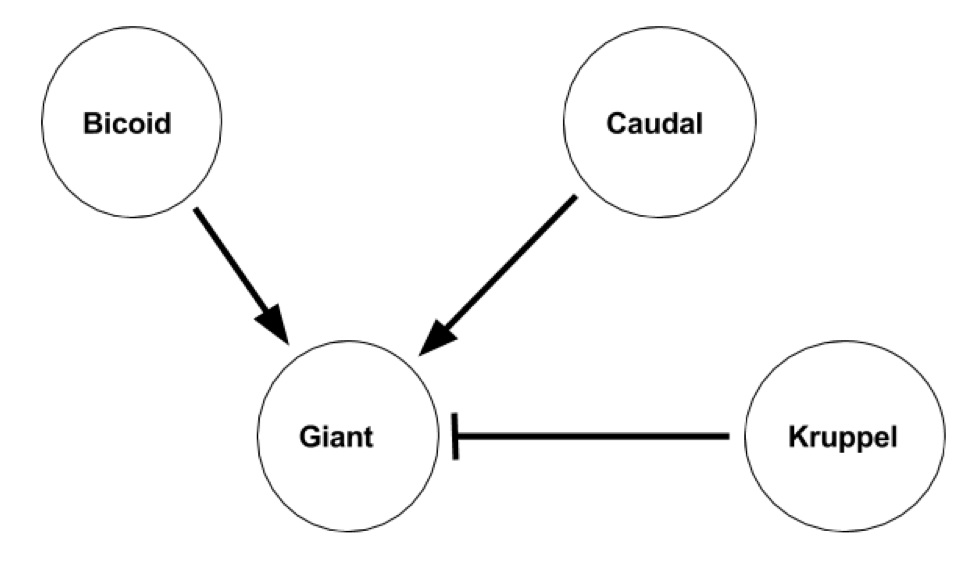
\includegraphics[scale=0.55]{embryo/giant_activation.png}
  \caption{Regulatory interactions of Giant. Giant is activated by the maternal genes, bicoid and caudal, in a OR manner. It is repressed by the gap gene, Kruppel.}
\label{fig:giant_activation}
\end{figure}
As depicted in fig. \ref{fig:giant_activation}, Giant (Gt) is activated by the presence of either of the maternal genes, Bicoid or Caudal, (OR activation). In addition, Giant is repressed by the action of of Kruppel. Based on this scheme, we can formulate the rate of Giant production as:
$$P^{Gt} = (1 - (1 - p^{Bcd})(1 - p^{Cad}))(1 - p^{Kr}),$$
\begin{align*}
P^{Gt} = &(1-\frac{C_o^{Bcd}}{C_o^{Bcd} + (1+C_o^{Bcd} K^{Bcd} [Bcd])^{N_s^{Bcd}} - 1}*\frac{C_o^{Cad}}{C_o^{Cad} + (1+C_o^{Cad} K^{Cad} [Cad])^{N_s^{Cad}} - 1})\\
&*(\frac{C_o^{Kr}}{C_o^{Kr} + (1+C_o^{Kr} K^{Kr} [Kr])^{N_s^{Kr}} - 1}).
\end{align*}

\subsubsection{Model Equations}
Assuming the constants defined in table \ref{tab:table1}, we provide the complete partial differential equations associated with each of the gap genes. \\
Hunchback (Hb):
\begin{align*}
\frac{\partial }{\partial x}[Hb] &= \alpha \left ( (1 - \frac{C_o}{C_o + (1 + C_oK_3[Bcd])^{N_s} -1})(1 - \frac{C_o}{C_o + (1 + C_oK[Hb])^{N_s} -1})\right )\\ & \left ( (\frac{C_o}{C_o + (1 + C_oK[Kni])^{N_s} -1}) \right )\\
&- \beta [Hb] + D/L^2 \frac{\partial^2 [Hb]}{\partial x^2}.
\end{align*}
Knirps (Kni):
\begin{align*}
\frac{\partial }{\partial x}[Kni] &= \alpha \left ( (1 - \frac{C_o}{C_o + (1 + C_oK_3[Bcd])^{N_s} -1})(\frac{C_o}{C_o + (1 + C_oK_1[Hb])^{N_s} -1})\right)\\& \left ( (\frac{C_o}{C_o + (1 + C_oK[Tll])^{N_s} -1}) \right )\\ 
&- \beta [Kni] + D/L^2 \frac{\partial^2 [Kni]}{\partial x^2}.
\end{align*}
Kruppel (Kr):
\begin{align*}
\frac{\partial }{\partial x}[Kr] &= \alpha \left ( (1 - \frac{C_o}{C_o + (1 + C_oK[Hb])^{N_s} -1})(\frac{C_o}{C_o + (1 + C_oK[Hb])^{N_s} -1})\right)\\&\left((\frac{C_o}{C_o + (1 + C_oK[Gt])^{N_s} -1}) \right )\\ 
&- \beta [Kr] + D/L^2 \frac{\partial^2 [Kr]}{\partial x^2}.
\end{align*}
Giant (Gt):
\begin{align*}
\frac{\partial }{\partial x}[Gt] &= \alpha  \biggl( (1 - (1 - \frac{C_o}{C_o + (1 + C_oK_3[Bcd])^{N_s} -1}*\frac{C_o}{C_o + (1 + C_oK[Hb])^{N_s} -1}))  \\
 &(\frac{C_o}{C_o + (1 + C_oK_2[Kr])^{N_s} -1})(\frac{C_o}{C_o + (1 + C_oK[Tll])^{N_s} -1}) \biggr) - \beta [Gt] + D/L^2 \frac{\partial^2 [Gt]}{\partial x^2}.
\end{align*}
To produce the base model A6, $K_3$ is set to equal $K$ and $K_2$ is set to equal $K_1$. Further models are derived according to specifications in Table 1 of the main section. To include the activation of kruppel by bicoid, the equation of kruppel above is modified to the following:
\begin{align*}
\frac{\partial }{\partial x}[Kr] &= \alpha \biggl ( (1 - \frac{C_o}{C_o + (1 + C_oK_3[Bcd])^{N_s} -1})(1 - \frac{C_o}{C_o + (1 + C_oK[Hb])^{N_s} -1})\\
&(\frac{C_o}{C_o + (1 + C_oK[Hb])^{N_s} -1})(\frac{C_o}{C_o + (1 + C_oK[Gt])^{N_s} -1}) \biggr ) - \beta [Kr] + D/L^2 \frac{\partial^2 [Kr]}{\partial x^2}.
\end{align*}

Here, $[Bcd], [Tll]$ are the concentrations of maternal genes bicoid and tailless respectively. All concentrations are function of space and time, i.e.:
$$[A] \equiv [A](x, t)$$

\subsubsection{Normalization}
We assume equal synthesis rates for all four gab genes. This value is also same as the deacy rate for each of the gap genes. Further, Papatsenko and Levine \cite{papatsenko11} assumed that the gap genes undergo similar activation at the beginning of their expression. This assumption can be handled by applying a normalization constant to the production term. Specifically, we pre-multiply the synthesis rate of gap gene $[A]$ with $\omega^A$:
\begin{align*}
\frac{\partial }{\partial t}[A] &= \omega^A \alpha P_{A}^{act}(1 - P_{A}^{rep}) - \beta [A] + D/L^2 \frac{\partial^2 [A]}{\partial x^2},\\
\omega^A &= \frac{1}{Max(P^{act}(x|t=0,K,C_o,N_s))}.
\end{align*}
\subsection{Model Solution}
We provide here the complete solution to the reaction-diffusion equation describing gap gene expression. We first do a change of variables to dimensionless space $x \rightarrow x/L$, where L is the length of the embryo, and rewrite the equation as:
\begin{align}
\frac{\partial }{\partial t}u_{i}(x,t) &= \alpha P_{i}^{A}(1 - P_{i}^{B}) - \beta u_{i}(x,t) + D/L^2 \frac{\partial^2 u_{i}(x,t)}{\partial x^2} ,\\ 
i &= Hb, Kr, Kni, Gt , \nonumber \\
u'(0,t) &= u'(1,t) = 0, u' =  \frac{\partial u}{\partial x} , \nonumber\\
0 &< x < 1, 0 < t < T. \nonumber
\end{align}
%\begin{eqnarray*}
%\frac{\partial }{\partial t}y_{i}(x,t) = \alpha P_{i}^{A}(1 - P_{i}^{B}) - \beta y_{i}(x,t) + D/L^2 %\frac{\partial^2 y_{i}(x,t)}{\partial x^2}, \\
%i = Hb, Kr, Kni, Gt\\
%0 < x < 1, 0 < t < T\\
%y'(0,t) = y'(1,t) = 0
%\end{eqnarray*}
Stated this way, the expression of gap genes is a system of non-linear partial differential equations (PDEs). For convenience, in the following derivation we drop the subscript $i$ and set $f = \alpha P_{i}^{A}(1 - P_{i}^{B})$ to capture the non-linearity in the system. The time differential of the concentration, $u$, is represented by $u_t$. Thus, we can write the above equation in the weak form as:
\begin{eqnarray*}
<u_t, v> &=& <f, v> - \beta <u, v> + D/L^2 <u_{xx}, v> .
\end{eqnarray*}
Integrating by parts, we can re-write the above as:
\begin{eqnarray*}
<u_t, v> &=& <f, v> - \beta <u, v> - D/L^2 <u_x, v_x>.
\end{eqnarray*}
We use the finite element subspace, $V_h = span \{ \phi _i | 1  \leq i \leq n\}$ and approximate the solution with $u^n = \sum_{j=0}^{n}u_j \phi _j$ where, for $i = 1 \cdots n-1$:
\begin{equation*}
    \phi_i(x) = 
\begin{cases}
    nx - (i-1) ,& \frac{i-1}{n} \leq x \leq \frac{i}{n}\\
    (i+1) - nx ,& \frac{i}{n} \leq x \leq \frac{i+1}{n}\\
    0,              & \text{otherwise}
\end{cases}
\end{equation*}
and
\begin{equation*}
    \phi_0(x) = 
\begin{cases}
    1 - nx ,& 0 \leq x \leq \frac{1}{n}\\
    0,              & \text{otherwise},
\end{cases}
\end{equation*}

\begin{equation*}
    \phi_n(x) = 
\begin{cases}
    nx - (n-1) ,& \frac{n-1}{n} \leq x \leq 1\\
    0,              & \text{otherwise}.
\end{cases}
\end{equation*}
Given the basis, we can write the finite element method as:
$$\sum_{j=0}^{n}(u_j)_t< \phi _j, \phi _i> = <f, \phi _i> - \sum_{j=0}^{n}u_j( \beta <\phi _j, \phi _i> + D/L^2 <\phi' _j, \phi' _i> ).$$ 
% say that u^n is the discrete case or projection into the finite element subspace
Rewriting in matrix form, where the superscript, $n$ , now indicates that we are working in the subspace $V_h$, 
\begin{eqnarray}
M^n u_t^n &=& -(\beta M^n + (D/L^2)K^n)u^n + F \nonumber \\
% describe these matrices. 
u_t^n &=& -(\beta I + (D/L^2)(M^n)^{-1}K^n)u^n + (M^n)^{-1} F \nonumber \\
u_t^n &=& -A^nu^n + F^n.
\end{eqnarray}
Here, $F = \left(<f, \phi_1>, <f, \phi_2>, \cdots, <f, \phi_n> \right )'$ and 
\begin{align*}
M^n &= [M^n_{ij}] = [<\phi_j, \phi_i>],\\
K^n &= [K^n_{ij}] = [<\phi'_j, \phi'_i>],\\
A^n &= \beta I + (D/L^2)(M^n)^{-1}K^n\\
F^n &= (M^n)^{-1} F.
\end{align*}
We can now use the integrating factor method to solve the above ordinary differential equation in (2.2). Consider an interval $\tau$ in which we study the system. We can divide the total time $T$ into $T/\tau$ such intervals and examine the system at the $k^{th}$ step where $u_k^n = u^n(k\tau )$. Using this formulation, we write:
% say that you are solving an ODE
\begin{eqnarray}
u^n_{k+1} &=& u^n((k+1)\tau ) \nonumber \\
&=& e^{A^n\tau }u^n(k\tau ) + \int_{k\tau }^{(k + 1)\tau } e^{A^n((k+1)\tau -s)}F^n(u^n(s))ds \nonumber \\ 
&\approx& e^{A^n\tau }u^n(k\tau ) + \int_{k\tau }^{(k + 1)\tau } e^{A^n((k+1)\tau -s)}dsF^n(u^n(k\tau )) \nonumber \\
&\approx& e^{A^n\tau }u^n(k\tau ) + \int_{0}^{\tau } e^{A^ns}dsF^n(u^n_k) \nonumber\\
\Rightarrow u^n_{k+1} &\approx& \Phi^n u^n_k + B^nF^n(u^n_k)
\end{eqnarray}
As $A^n$ is invertible, the integral $B^n = \int_{0}^{\tau } e^{A^ns}ds$ is evaluated to be $(A^n)^{-1}(e^{A^n\tau} - I)$. Equation (2.3) now provides an iterative solution for the PDE expressed in (2.1).


\subsection{Parameter Estimation}
The observed data is assumed to have some noise $\epsilon$, which we take to be identically normally distributed, $\epsilon \sim N(0, \sigma ^2I)$, (where $I$ is the identity matrix). If the observed data is $Y$ and $U$ is the solution to the system of PDEs, we have:
\begin{align*}
Y_{i} &= U_{i}(x,T) + \epsilon, \\
i &= Hb, Kr, Kni, Gt, \\
0 &< x < L.
\end{align*}

Following the above formulation, we can define the likelihood function, $L(\theta, Y)$, which gives the conditional probability of the data, $Y$, given the parameter, $\theta$. Here we have the dropped the subscript $i$ for gap genes for the sake of convenience. Given the assumed error model, the likelihood can be written down explicitly as 
$$L(\theta, Y) = p(Y | \theta)  = \prod_{j=1}^{N} \frac{1}{\sqrt{2 \pi \sigma ^2}} \textup{exp}(-\frac{1}{2 \sigma ^2}(y_j - u_j)^2).$$

We note that we apply the error model for specific domains over the embryo length (e.l.) . Specifically, the domains used for the gap genes are 30-70 \% e.l. for Hb, 40-90 \% e.l. for Kni, 20-80 \% e.l. for Kr and 10-90 \% e.l. for Gt. The posterior incorporates both how well the parameters support the data and also our existing knowledge of them. This can be expressed more mathematically using Bayes' theorem \cite{bayes63}:
$$p(\theta | Y) = \frac{L(\theta, Y) \pi(\theta )}{p(Y)}$$
where
\begin{itemize}
\item $p(\theta | Y)$ is the posterior density of the parameters
\item $L(\theta; Y)$ is the likelihood of the data as elaborated above
\item $\pi (\theta )$ is the prior belief of the parameter
\item $p(Y)$ is the marginal likelihood 
\end{itemize}

At first glance, it would appear straightforward to use Bayes' theorem to compute the posterior density of the parameters. However, the marginal likelihood term in the denominator is often hard to evaluate numerically and mostly intractable as it involves an integration of the likelihood over the whole parameter space:

$$p(Y) = \int_{\Theta} L(\theta, Y) \pi(\theta ) d\theta .$$

Instead, we rely on the Markov chain Monte Carlo \cite{gilks95} method used for high-dimensional sampling. The idea behind these methods is to draw samples from the stationary distribution of a Markov chain. When set up correctly, this distribution produces samples from the posterior distribution. The marginal likelihood itself, however, is relevant for model selection and we will return to its estimation in the section on model selection.

\subsubsection{Metropolis-Hastings Sampling}

The Metropolis-Hastings algorithm \cite{hastings70} provides a procedure to draw samples from the target distribution based on a proposal density. When the appropriate target density is defined, this amounts to generating samples from the posterior distribution of the dynamic model of interest. The MH algorithm achieves this by suggesting moves based on a proposal distribution, $q(\theta _{i+1}|\theta _{i})$, for the Markov chain which proposes a new value for $\theta_{i+1}$ conditional on the current value of $\theta_i$. These moves are accepted based on the Hastings ratio:

$$a_{hr} = min\left \{ 1, \frac{p(\theta _{i+1}| Y) q(\theta _{i}| \theta _{i+1})}{p(\theta _{i}| Y) q(\theta _{i+1}| \theta _{i})} \right \} = min\left \{ 1, \frac{L(\theta _{i+1}, Y) \pi(\theta _{i+1})q(\theta _{i}| \theta _{i+1})}{L(\theta _{i}, Y) \pi(\theta _{i})q(\theta _{i+1}| \theta _{i})} \right \} .$$

The terms are as defined previously and we note that the marginal likelihood term has conveniently canceled out in denominator. The proposal $q(\cdot | \cdot)$ is usually taken to be a Gaussian, however, we note that in our case, the number of sites parameter, $N_s$, is discrete. Accordingly, we define the proposal density as a mixed density. With probability, $p < 1/10$, we perturb $N_s$ by either increasing or decreasing it by 1 with equal probability, while keeping the rest of the parameters unchanged. Else, we perturb each of the other parameters based on a Gaussian centered at the current value of the parameters, $\theta _{i}$ and with variance $0.1I$, where I is the identity matrix. We use bounded uniform prior on all the parameters.

\subsubsection{Parallel Tempered MCMC Sampling}

In principle, given a large number of samples, the Metropolis-Hastings sampler should be able to cover the whole parameter space. However, in high dimensions, the number of samples required increases rapidly and there is always the chance of the chain getting stuck in local optima. To get around these issues, it has been proposed to use multiple interacting MCMC chains \cite{geyer91}. One such approach is of parallel tempering where parallel MCMC chains are run at different 'temperatures'. The range of temperatures that are used is referred to as the temperature ladder. The likelihood for a chain at temperature $t$ is now given by:

$$L_{t}(\theta, Y) = p_{t}(Y| \theta) = p(Y| \theta)^{t}.$$

Since the likelihood function is smoother for higher temperatures, chains at higher temperature can sample the parameter space more freely. The chains are updated using a Metropolis Hastings update step and chains at neighbouring temperatures are exchanged using an acceptance ratio. For implementation purposes, we follow the approach in \cite{calderhead12} with a slight modification. Algorithmically:

\begin{enumerate}
\item Initial start positions are assigned to each chain, $\Theta = (\theta_{1}, \ldots, \theta_{N})$
\item Associate each chain with a temperature based on a temperature ladder, $(\Theta, t) = (\theta_{1}, t_{1}, \ldots \theta_{N}, t_{N})$
\item Repeat till convergence of all chains
\begin{enumerate}
\item Apply local Metropolis-Hastings update step to each chain
\item Pick two neighboring chains at different temperature. Assume states $\theta_{i}$ and $\theta_{j}$ for N pairs $(i, j)$ with $i$ sampled uniformly in $(1, \ldots , N)$ and $j=i \pm 1$ with probability $p_{e}(\theta_i, \theta_j)$ where $p_{e}(\theta_i, \theta_{i+1}) = p_{e}(\theta_i, \theta_{i-1}) = 0.5$ and $p_{e}(\theta_{1}, \theta_2) = p_{e}(\theta_{N}, \theta_{N-1}) = 1$
\item Exchange the state of the chains based on acceptance ratio
\end{enumerate}
\item Use chain with lowest temperature for estimating posterior density
\end{enumerate}

The exchange step is accepted with probability $min(1, a_{e})$ according to the Metropolis-Hastings rule:

$$a_{e} = \frac{p(\Theta '|Y)Q(\Theta | \Theta ')}{p(\Theta |Y)Q(\Theta '| \Theta)} = \frac{[L(\theta_{j},Y)^{t_i}*L(\theta_{i},Y)^{t_j}]}{[L(\theta_{i},Y)^{t_i}*L(\theta_{j},Y)^{t_j}]}* \frac{Q(\Theta | \Theta ')}{Q(\Theta '| \Theta)}$$

where $Q(\cdot |\cdot )$ denotes the probability of transition from a set of chains to a set with a neighboring pair of chains exchanged. We select direct neighbors in the temperature ladder for the exchange step to increase the likelihood for the exchange to be accepted. 

While the chain at the lowest temperature can be used for parameter inference, all the chains together can be used to estimate the marginal likelihood \cite{calderhead10} and in turn calculate Bayes factors for Bayesian model comparison for model ranking. After providing an example to illustrate the benefits of PT-MCMC, we turn to the aspect of model selection.

\subsubsection{Example}

To see the power of the PT-MCMC approach, we generate samples from a test function as suggested by Wilkinson \cite{wilkinson}. This test function corresponds to the density function of the double-well potential:

$$\rho(x) \propto exp \left \{ - \gamma (x^2 - 1)^2 \right \}.$$

The density function is inspired from a physical setting but those details are not important to us. We plot in fig. \ref{fig:density} the shape of the density plot for $\gamma = 4$.

\begin{figure}[h!]
\centering
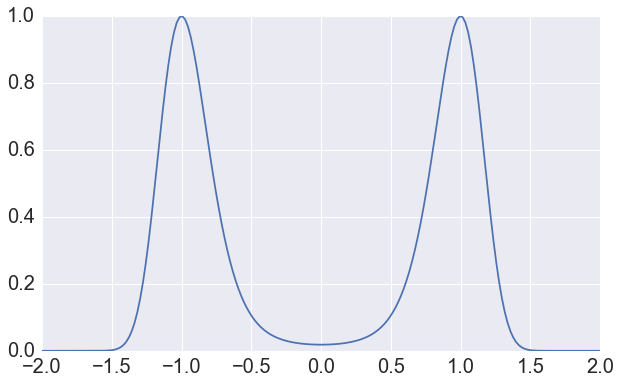
\includegraphics[scale=0.55]{embryo/density_plot.png}
\caption{Unnormalized density function for the double potential well. ($\gamma = 4$)}
\label{fig:density}
\end{figure}

We note that the density function has two modes and the strength of the separation of the two modes depends on the $\gamma$ parameter. Higher the value of the gamma parameter, the more separated are the modes. Thus, we expect that at higher values of $\gamma$, it would be increasingly difficult to recover the true distribution using a MH-MCMC sampler. This is because there is an higher possibility of a sampler getting stuck in one of the two modes. 

To test this idea we ran 10,000 iterations for each sampler, MH-MCMC and PT-MCMC. The results are shown in fig. \ref{fig:mh-mcmc} and fig. \ref{fig:pt-mcmc} for MH-MCMC and PT-MCMC respectively. The first column in these figures shows the true distribution that we want to sample from. This represents the density function of the double-well potential with increasing $\gamma$. As can be seen, the two modes of the function get more and more isolated as $\gamma$ increases. A good diagnostic of convergence is the trace plot which is the time series of the samples from the MCMC sampler. This has been plotted in the third column. Finally, we plot the distribution recovered from each sampler in the second column. 

As can be seen in fig. \ref{fig:mh-mcmc}, at a $\gamma$ value of 8, the MH-MCMC sampler has difficulty sampling from the true distribution and starts rapidly switching between the two modes. At a $\gamma$ value of 16, the MH-MCMC sampler samples only from one mode. What is worse is that looking at the corresponding trace plot, one could surmise that convergence has been achieved which would be erroneous. In contrast, looking at fig. \ref{fig:pt-mcmc}, we can see that the PT-MCMC has no difficulty to sample from the true distribution at all values of $\gamma$. Furthermore, the trace plot indicates that convergence has been truly reached. 

\begin{figure}[h!]
\centering
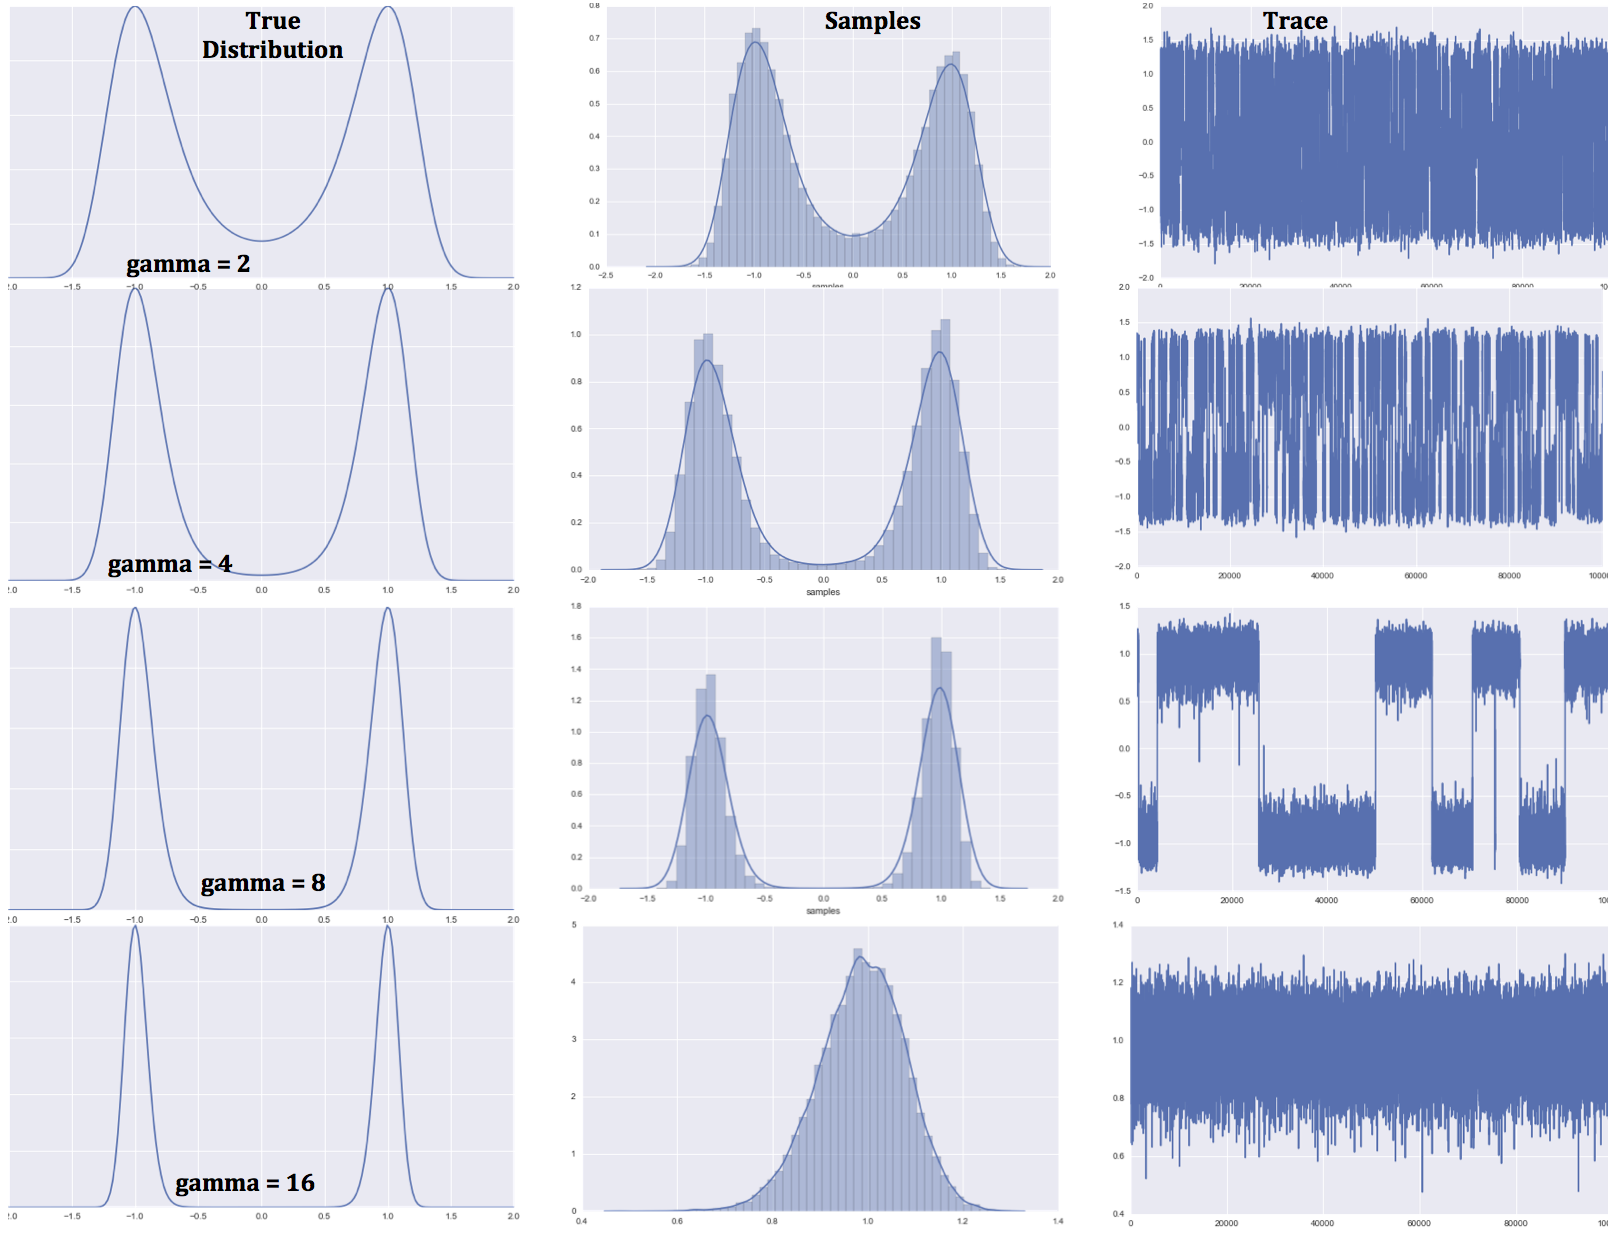
\includegraphics[scale=0.55]{tex/embryo/dble_potn_well.png}
\caption{Metropolis-Hastings (MH-MCMC) sampling for the density of the double potential well.}
\label{fig:mh-mcmc}
\end{figure}

\begin{figure}[h!]
\centering
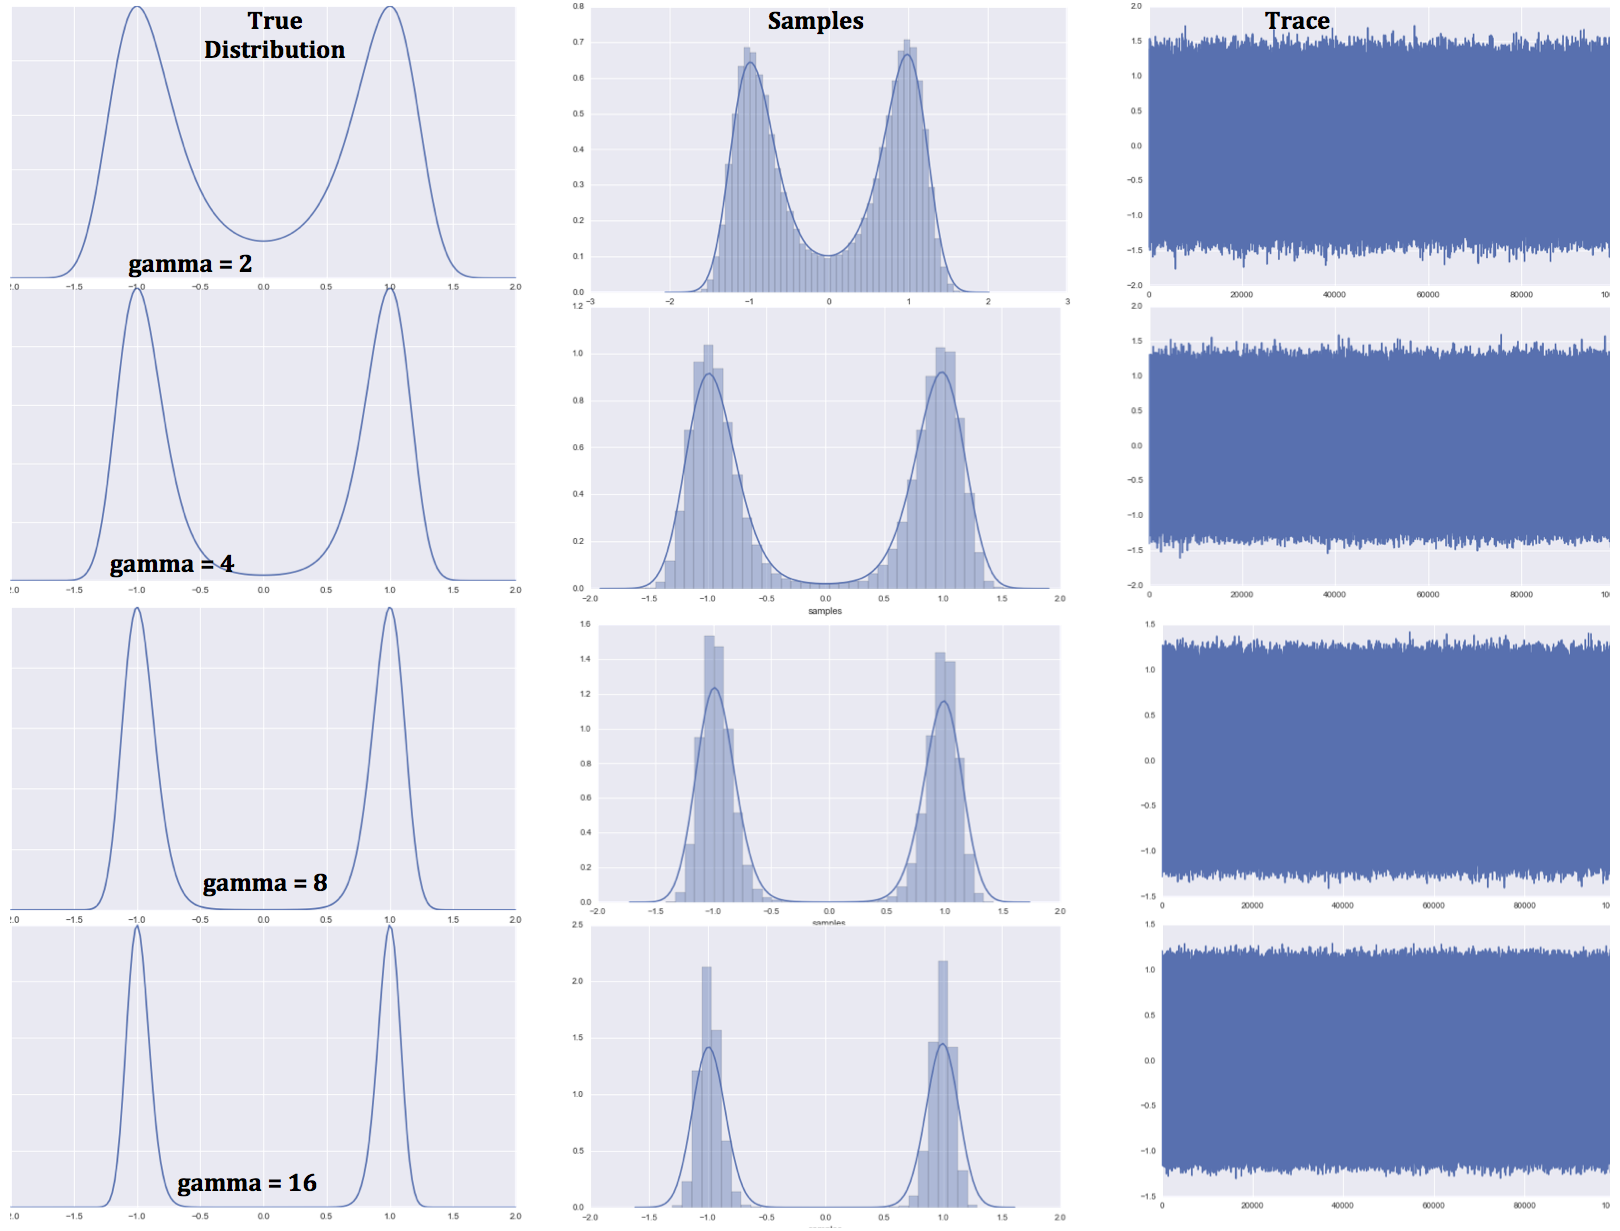
\includegraphics[scale=0.55]{tex/embryo/dble_potn_well_ptmcmc.png}
\caption{PT-MCMC sampling for the density of the double potential well.}
\label{fig:pt-mcmc}
\end{figure}

\subsection {Model Selection}

In the context of Bayesian inference, Bayes factors can be employed to do model selection. They allow us to compute the posterior probabilities of two models, given the prior probability of each model. Assuming again that the data is $Y$, and we want to compare between two models, $M_{1}$ and $M_{2}$, then the posterior odds are given by:

$$\frac{p(M_1|Y)}{p(M_2|Y)} = \left (\frac{p(Y|M_{1})}{p(Y|M_{2})}  \right ) \frac{p(M_1)}{p(M_2)}.$$

The quantity in brackets is the ratio of the marginal likelihoods of the two models and is termed the Bayes factors. When we have no prior preference of one model over the other, we assume $p(M_1) = p(M_2)$ and then the ratio of likelihoods is exactly equal to the Bayes factor. In essence, then, the problem of model selection boils down to the problem of estimating the marginal likelihood.

Various methods to estimate the marginal likelihood have been proposed \cite{girolami08a, girolami08b}. In the simplest construction, given samples from the prior $\theta_1 ,\theta_2 , ..., \theta_n $, one could compute the Monte Carlo estimate

$$\hat{p}(Y) = \frac{1}{n}\sum_{i=1}^{n}p(Y|\theta_i).$$

However, in practice this is a poor estimator unless working with very large sample sizes. Similarly, the importance sampling based the posterior harmonic mean estimator has been shown \cite{girolami08b, meng96} to be a very poor estimator. 

Instead, we could exploit the tempered distributions that we have generated using the PT-MCMC sampler. This approach has been referred to as path sampling \cite{meng96, meng98}. If we assume that the marginal likelihood of chain at temperature $t$ is represented as $z_t$, then:

%$$p(Y) = z_N = \frac{z_1}{z_0}\cdot\frac{z_2}{z_1}\cdots\frac{z_N}{z_{N-1}}$$
%where 
%$$\frac{z_{i+1}}{z_i} = \frac{\int_{\Theta} p(\theta) p(y|\theta)^{t_i+1}d\theta}{z_i} = \int_{\Theta}p(y|\theta)^{t_{i+1} - t_i} \cdot \frac{p(y|\theta)^t_i p(\theta)}{z_i} d\theta = E_i[p(y|\theta)^{t_{i+1} - t_i}]$$

$$z_t = z(t) = \int_{\Theta} p(Y|\theta)^{t}\pi(\theta) d\theta .$$

By differentiating the logarithm of $z$,

$$\frac{d}{dt}\text{log}z_t = \int_{\Theta}\text{log}(p(Y|\theta)) \cdot \frac{p(Y|\theta)^t \pi(\theta)}{z_t} d\theta = E_t[\text{log}(p(Y|\theta))]$$

and then we can integrate both sides with respect to $t$ to obtain:

$$\text{log}(p(Y)) = \int_{0}^{1}E_t[\text{log}(p(Y|\theta))]dt$$ 

as described in \cite{girolami08a}. Thus, if we choose a temperature ladder $(0 = t_0 < t_1 < t_2 < ... < t_{N-1} < t_N = 1)$, then we can use a numerical approximation to compute the above integral. Namely, 
$$\text{log}(p(Y)) = \sum_{i=1}^{N-1}0.5(t_{i+1} - t_i)\left \{ E_{t_{i+1}}[\text{log}(p(Y|\theta))] + E_{t_{i}}[\text{log}(p(Y|\theta))] \right \}.$$
The expectation with respect to the posterior at each temperature on the ladder can be approximated using the Monte Carlo estimate. For all the models we used a temperature schedule with $N = 10$ according to an exponential ladder $t_i = (\frac{i}{N})^5, i = 1, ..., N$ as suggested in \cite{calderhead10}.
%Thus, working with the $log$ of the marginal likelihood, we can write:
%$$\textup{log}p(Y) = \sum_{i=0}^{N-1}\textup{log}\frac{z_{i+1}}{z_i} = \sum_{i=0}^{N-1}\textup{log}E_i[p(y|\theta)^{t_{i+1} - t_i}]$$
%$$= \sum_{i=0}^{N-1}\textup{log}E_i[\textup{exp}\left \{ (t_{i+1} - t_i) \textup{log} p(y|\theta) \right \}]$$
%$$\approx \sum_{i=0}^{N-1}(t_{i+1}-t_i)E_i[\textup{log}p(y|\theta)]$$
%The above formula can then be used to estimate the marginal likelihood and hence, to obtain estimates of the Bayes Factor between two competing models.

\subsection{Model Over-fitting}

The process of model selection described above helps guard against choosing over-parameterized models by penalizing them implicitly for higher dimensionality. This ability of Bayes factors to prioritize simpler models over complex ones has also been discussed elsewhere \cite{jeffreys92,girolami08a}. 

However, as we consider relative goodness of fit amongst models, there might still be an argument that the best chosen model does over-fit the data. One way to test model over-fitting is cross-validation \cite{Kohavi95astudy}. In such an approach, usually, we can envisage excluding some of the data (validation set) during model fitting step  and then testing the accuracy of the model on this held-out data set. An over-fit model would perform well on the fitted data but poorly on the held-out dataset. 

However, as we deal with a spatially correlated dataset, cross-validation becomes more difficult as leaving out an observation does not remove all the associated information. In order to compute a cross-validation statistic, we use an iterative procedure. We use the mean log-likelihood as a measure of prediction accuracy. 

\begin{enumerate}
\item We fit the model to the data $y_1, \cdots, y_m$, where $m$ is chosen such that $1, \cdots, m$ corresponds to the first 60\% of the data, drawn sequentially across the embryo axis.
\item We use the fitted model to predict for the next 5\% of observations and compute the log-likelihood.
\item Repeat steps 1 \& 2, adding 5\% of the data set to training set and predict the next 5\%. 
\item Finally, compute the mean log-likelihood from the predictions made above.
\end{enumerate}

As our data is stratified, we ensure that the training set draws evenly from expression observation of the gap genes, i.e. we pick the initial 60\% of the observations from each of the four gap genes to train the model. Similarly, predictions are made on the next 5\% of the observations for each gap gene.

The models, solver and MCMC sampler were coded using the python programming language. PyMC \cite{patil10} was used for certain diagnostic visualizations. The code for reproducing the analysis is available on GitHub at the repository:\\ \href{https://github.com/asifzubair/BayesianModelSelection}{https://github.com/asifzubair/BayesianModelSelection}. 

\section{Results and Discussion}

The \textit{Drosophila} gap gene network has been the subject of intense study from both experimentalists and computational modelers. Despite this, efforts to compare proposed network hypothesis in a statistically rigorous manner have been few and far between. Here, we propose to use the Bayesian framework for doing parameter inference and model selection. The Bayesian framework permits one to do a fully probabilistic analysis of model system allowing one to account for uncertainty in parameter estimates and model fit. We employ an MCMC approach using the parallel tempering (PT-MCMC) sampler to do Bayesian analysis. This sampler not only allows for better convergence but also helps one to compute the thermodynamic estimator for marginal likelihood. Other sampling approaches for accelerating convergence like adaptive MCMC \cite{Andrieu2008} and Hamiltonian Monte Carlo (HMC) \cite{Betancourt_A_2017} exist. However, these samplers require all the parameters to be continuous whereas the PT-MCMC sampler does not have such a restriction. In addition, they do not have the benefit of providing a natural way to estimate the marginal likelihood like the PT-MCMC sampler does. Using estimates of the marginal likelihood, we use Bayes factor to compare between models. 

Papatsenko \& Levine  argued that if the gene expression model is robust to the parameter values, then a single set of robust parameters should provide good model fits. In keeping with this, we set parameters related to maximal synthesis ($\alpha$),  decay ($\beta$), cooperativity rates ($C_o$) and diffusion ($D$) to be the same for all gap genes. In addition, we set the number of binding sites ($N_s$) to be the same. This forms the base model of 6 parameters (Model A6). Thereafter, we introduce node specific parameters to account for unequal mutual repression between Hb-Kni ($K_1$) and Gt-Kr ($K_2$). This is Model B7. We further test the possibility of the node-specific parameter ($K_3$) controlling Bicoid activation of three gap genes - Knirps, Hunchback and Giant. This is Model C8. In addition to this, certain studies have indicated the possibility of Bicoid activating Kruppel {\cite{knipple85, Becker13}, we also test for the evidence of this} by adding an extra edge to Models B7 and C8. These are models D7 and D8. All model specifications are described in table 1.

\begin{figure}
    \centering
    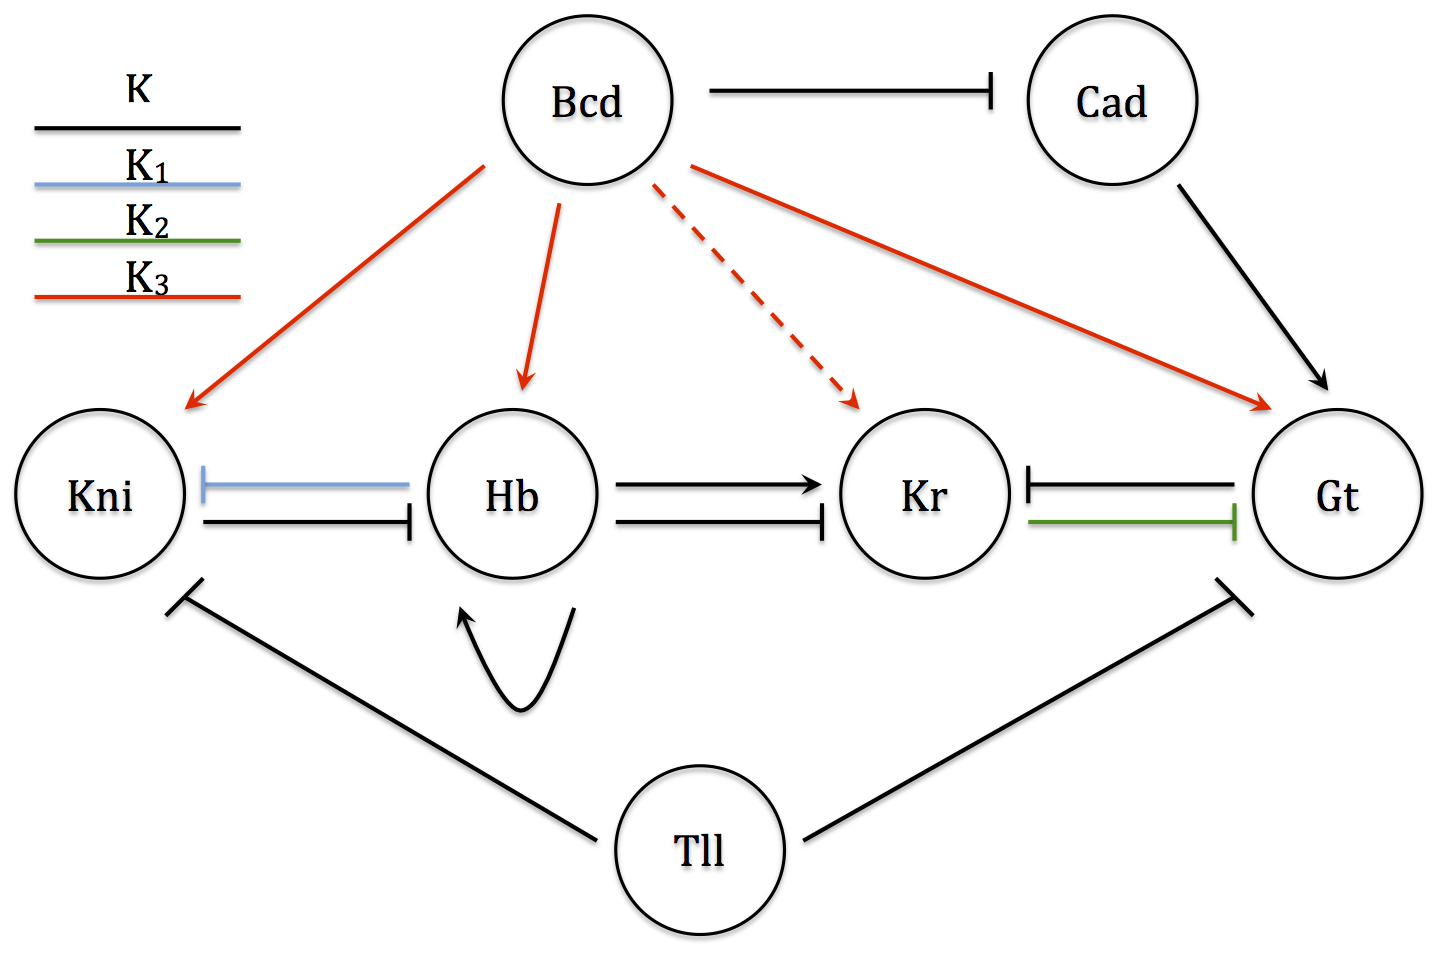
\includegraphics[height = 10cm, width = 10cm]{tex/embryo/figure-2.png}
    \caption{Gap gene network showing regulatory interactions between maternal genes, Bicoid (Bcd) \& Caudal (Cad), and gap genes (Knirps (Kni), Hunchback (Hb), Kruppel (Kr), Giant (Gt)). Two types of binding affinity parameters are shown - global (K) and edge-specific ($K_1, K_2, K_3$). We also investigate evidence for Bicoid activation of Kruppel (shown as dashed arrow).}
    \label{fig:figure-2}
\end{figure}


\begin{table}[h]
\centering

\begin{tabular}{lllllll}
\hline
\multicolumn{1}{l|}{Models} & \multicolumn{1}{l|}{A6} & \multicolumn{1}{l|}{B7} & \multicolumn{1}{l|}{B7r} & \multicolumn{1}{l|}{C8} & \multicolumn{1}{l|}{D7} & \multicolumn{1}{l}{D8} \\ \hline
\multicolumn{7}{l}{Global parameters:} \\ \hline
Affinity(logKa) & $K$   & $K$   & $K$   &        $K$               &            $K$          &           $K$ \\
Cooperativity   & $C_o$ & $C_o$ & $C_o$ &       $C_o$                &               $C_o$        &           $C_o$            \\
Binding Sites   & $N_s$ & $N_s$ & $N_s$ &             $N_s$          &            $N_s$           &             $N_s$          \\
Syn./Decay      & $\alpha$ & $\alpha$ & $\alpha$                   &     $\alpha$                  &        $\alpha$               &      $\alpha$                 \\
Diffusion       & D & D & D &            D           &                 D      &               D        \\
Max. conc       & 50 & 50 &           50            &          50             &          50             &         50              \\ \hline
%\multicolumn{7}{|l|}{Node-specific binding affinities:}
\multicolumn{7}{l}{Node-specific binding affinities:}                             \\ \hline
$Bcd^A$  & \textcolor{gray}{$K$} & \textcolor{gray}{$K$} & \textcolor{red}{$K_3$} & \textcolor{red}{$K_3$} & \textcolor{gray}{$K$} & \textcolor{red}{$K_3$} \\
$Bcd^R$                       &      \textcolor{gray}{$K$}                  &             \textcolor{gray}{$K$}           &       \textcolor{gray}{$K$}                 &      \textcolor{gray}{$K$}                  &       \textcolor{gray}{$K$}                 &         \textcolor{gray}{$K$}               \\
$Cad^A$                       &      \textcolor{gray}{$K$}                  &                \textcolor{gray}{$K$}        &     \textcolor{gray}{$K$}                   &         \textcolor{gray}{$K$}              &             \textcolor{gray}{$K$}           &          \textcolor{gray}{$K$}              \\
$Hb^A$                       &         \textcolor{gray}{$K$}               &             \textcolor{gray}{$K$}           &        \textcolor{gray}{$K$}                &          \textcolor{gray}{$K$}              &        \textcolor{gray}{$K$}                &        \textcolor{gray}{$K$}                \\
$Hb^D$                       &       \textcolor{gray}{$K$}                 &          \textcolor{gray}{$K$}              &      \textcolor{gray}{$K$}                  &           \textcolor{gray}{$K$}             &          \textcolor{gray}{$K$}              &           \textcolor{gray}{$K$}             \\
$Hb^R$                       &         \textcolor{blue}{$K_1$}               &           \textcolor{blue}{$K_1$}             &       \textcolor{blue}{$K_1$}                &              \textcolor{blue}{$K_1$}          &         \textcolor{blue}{$K_1$}              &       \textcolor{blue}{$K_1$}                 \\
$Gt^R$                       &     \textcolor{gray}{$K$}                  &              \textcolor{gray}{$K$}          &      \textcolor{gray}{$K$}                  &            \textcolor{gray}{$K$}            &        \textcolor{gray}{$K$}                &      \textcolor{gray}{$K$}                  \\
$Kr^R$                       &          \textcolor{gray}{$K_1$}              &              \textcolor{green}{$K_2$}          &       \textcolor{gray}{$K_1$}                 &             \textcolor{green}{$K_2$}           &           \textcolor{green}{$K_2$}             &         \textcolor{green}{$K_2$}               \\
$Kni^R$                       &        \textcolor{gray}{$K$}                &         \textcolor{gray}{$K$}               &       \textcolor{gray}{$K$}                 &             \textcolor{gray}{$K$}           &           \textcolor{gray}{$K$}             &         \textcolor{gray}{$K$}               \\
$Tll^R$                       &      \textcolor{gray}{$K$}                  &         \textcolor{gray}{$K$}               &        \textcolor{gray}{$K$}                &                \textcolor{gray}{$K$}        &            \textcolor{gray}{$K$}            &         \textcolor{gray}{$K$}               \\ \hline
Open Parameters:  &  6  &          7             &       7                &           8            &           7            &             8          \\ \hline
\end{tabular}
\vspace{0.25in}
\caption{Specifications for all 6 models evaluated. Models D7 and D8 have an extra edge for the activation of Bicoid by Kruppel. Also shown is the break up of global and node-specific parameters for different models. $Hb^{D}$ indicates parameter for the dual regulatory action of Hunchback on Kruppel.}
\label{tab:table1}
\end{table}


In their paper, Papatsenko \& Levine \cite{papatsenko11} fit each of the models (A6, B7 and C8) separately by maximizing an objective function based on the correlation measured between the model and the data. They use the final correlation value to distinguish between the models. Their formulation and analysis showed that the gap gene network can be modeled using a more modular approach, involving two relatively independent network domains. In addition, they show close agreement of parameter estimates and experimentally observed values for most parameters. However, their approach to compare the models themselves is slightly problematic as it does not apply appropriate penalties for increasing model dimensionality. Bayes factors apply this penalty implicitly and so adhere to the notion of Occam's razor of favoring simple hypothesis over complex ones. Moreover, Papatsenko \& Levine do not offer a measure of statistical significance to justify model choice and rely on an ad-hoc notion of over-fitting. We enhance their fundamentally sound approach by allowing for statistically rigorous model selection and also allow for comparing competing network hypothesis. 

\subsection{Efficient model solver}
The approach of Papatsenko \& Levine for solving the system of partial differential equations was to use a forward Euler integration loop in which diffusion is simulated by a Gaussian filter. However, the implementation of the solver was much too slow for a Bayesian analysis, where one may have to run upwards of a million iterations. To overcome this, we solved the system by the method of semi-groups. This gives rise to an iterative solution that can easily be vectorized and is numerically efficient. Our solver is an order of magnitude faster than the solver due to Papatsenko \& Levine (fig. \ref{fig:runtime}).

\begin{figure}[h!]
\centering
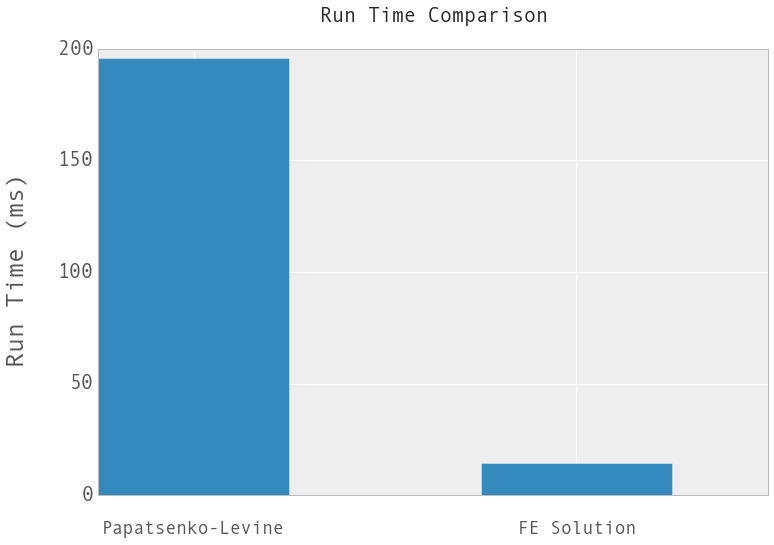
\includegraphics[scale=0.55]{tex/embryo/runtime.png}
\caption{Unnormalized density function for the double potential well. ($\gamma = 4$)}
\label{fig:runtime}
\end{figure}

\subsection{Fitting to simulated data \& identifiability}
\begin{figure}[h!]
\centering
	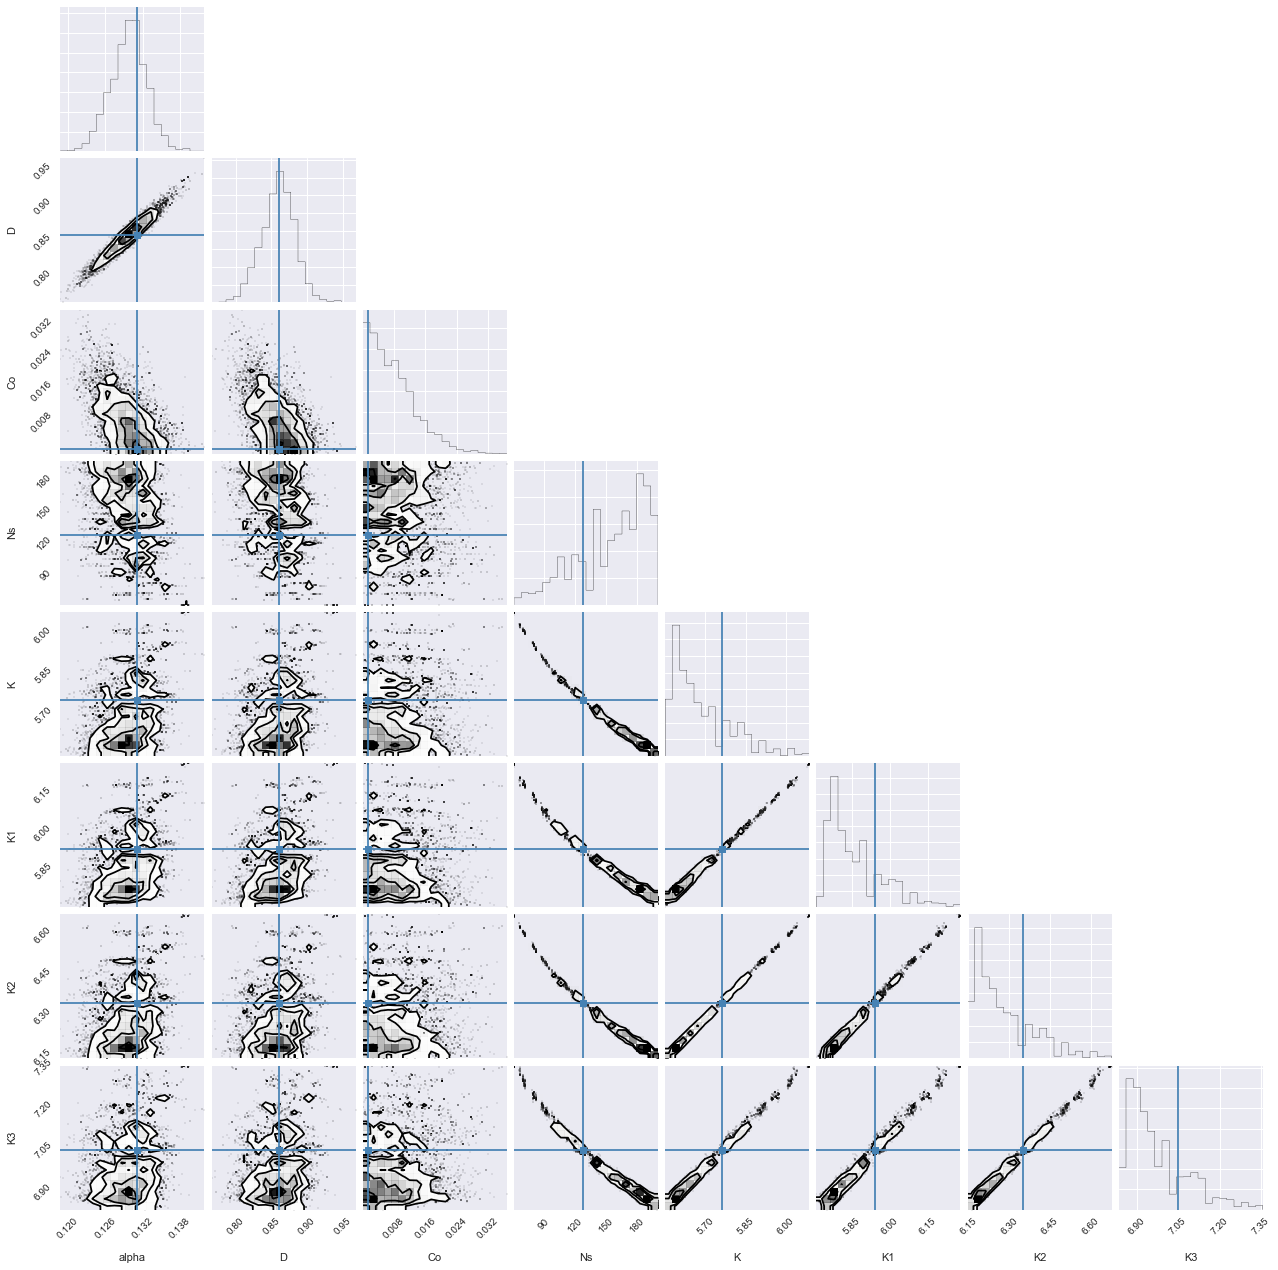
\includegraphics[height = 15cm, width =15cm]{tex/embryo/corner.png}
\caption{Corner plot \cite{corner} showing pair-wise joint densities of parameter for model C8. Simulated data, generated by adding noise to the output of the model with known parameters, was used to fit the model. The true values of the parameters are shown with blue lines. We see a strong negative correlation between the number of binding sites parameters, $N_s$, and the binding affinity parameters, $K, K_1, K_2, K_3$.}
\label{fig:corner}
\end{figure}

To investigate the structural properties of the Papatsenko-Levine formalism, we fit the  model C8 (largest number of parameters) to simulated data generated with a known parameter set. The simulated data is contaminated with Gaussian noise having zero mean and 0.1 variance. The parallel tempering sampler was used to fit the model to simulated data using 100,000 generations. As can be seen in fig.  \ref{fig:corner}, the parameters $\alpha$, $D$ and $Co$ are recovered and show no confounding. However, it can be seen that the parameter for number of sites parameters ($Ns$) is negatively correlated with binding affinities ($K1$, $K2$, $K3$). The binding affinities themselves are positively correlated. This points towards structural identifiability issues, but also is slightly intuitive as weaker binding affinity can be compensated by a increase in the number of `weak' binding sites. We also want to point out that any identifiability issues can be integrated out in the calculation of the marginal likelihood in a Bayesian framework and as such model selection can still be performed.

\subsection{Convergence of MCMC runs}

Time to convergence for MCMC samplers can be sensitive to initial start points. To overcome this, some approaches try to initialize the sampler from the MLE estimate of the likelihood function. This approach suffers from the same pitfalls as optimization algorithms, in that the sampler may not sample the whole likelihood space and the evidence of convergence may be misleading.

To ensure that the sampler had indeed converged, we initialized the chain from random start points drawn from a uniform prior. We used the Gelman-Rubin statistic \cite{brooks97} to monitor convergence of the chains. This diagnostic uses multiple chains to check for lack of convergence, and is based on the notion that if multiple chains have converged, by definition they should appear very similar to one another. The Gelman-Rubin statistic uses an analysis of variance approach to assessing convergence by calculating both the between-chain variance and within-chain variance to assess whether chains have indeed converged. We used the gelman.plot() function from the R \cite{r08} package coda \cite{plummer06} to plot the Gelman-Rubin statistic. It calculates the Gelman-Rubin shrink factor ($R$) repeatedly, first calculating with 50 observations and then adding bins of 10 observations iteratively. For convergence, we would ideally want the shrink factor to be below 1.2. 

Posteriors samples generated by fitting the data to simulated data showed evidence of confounding between a set of parameters (fig. \ref{fig:corner}). So, we used the convergence criteria on the likelihoods of the models. Figure \ref{fig:figure-3} shows the gelman-rubin statistic for four models. We see that the shrink factor drops sharply with number of iterations of the chain for all models. This implies that the chains have, indeed, converged. 

\begin{figure}[h!]
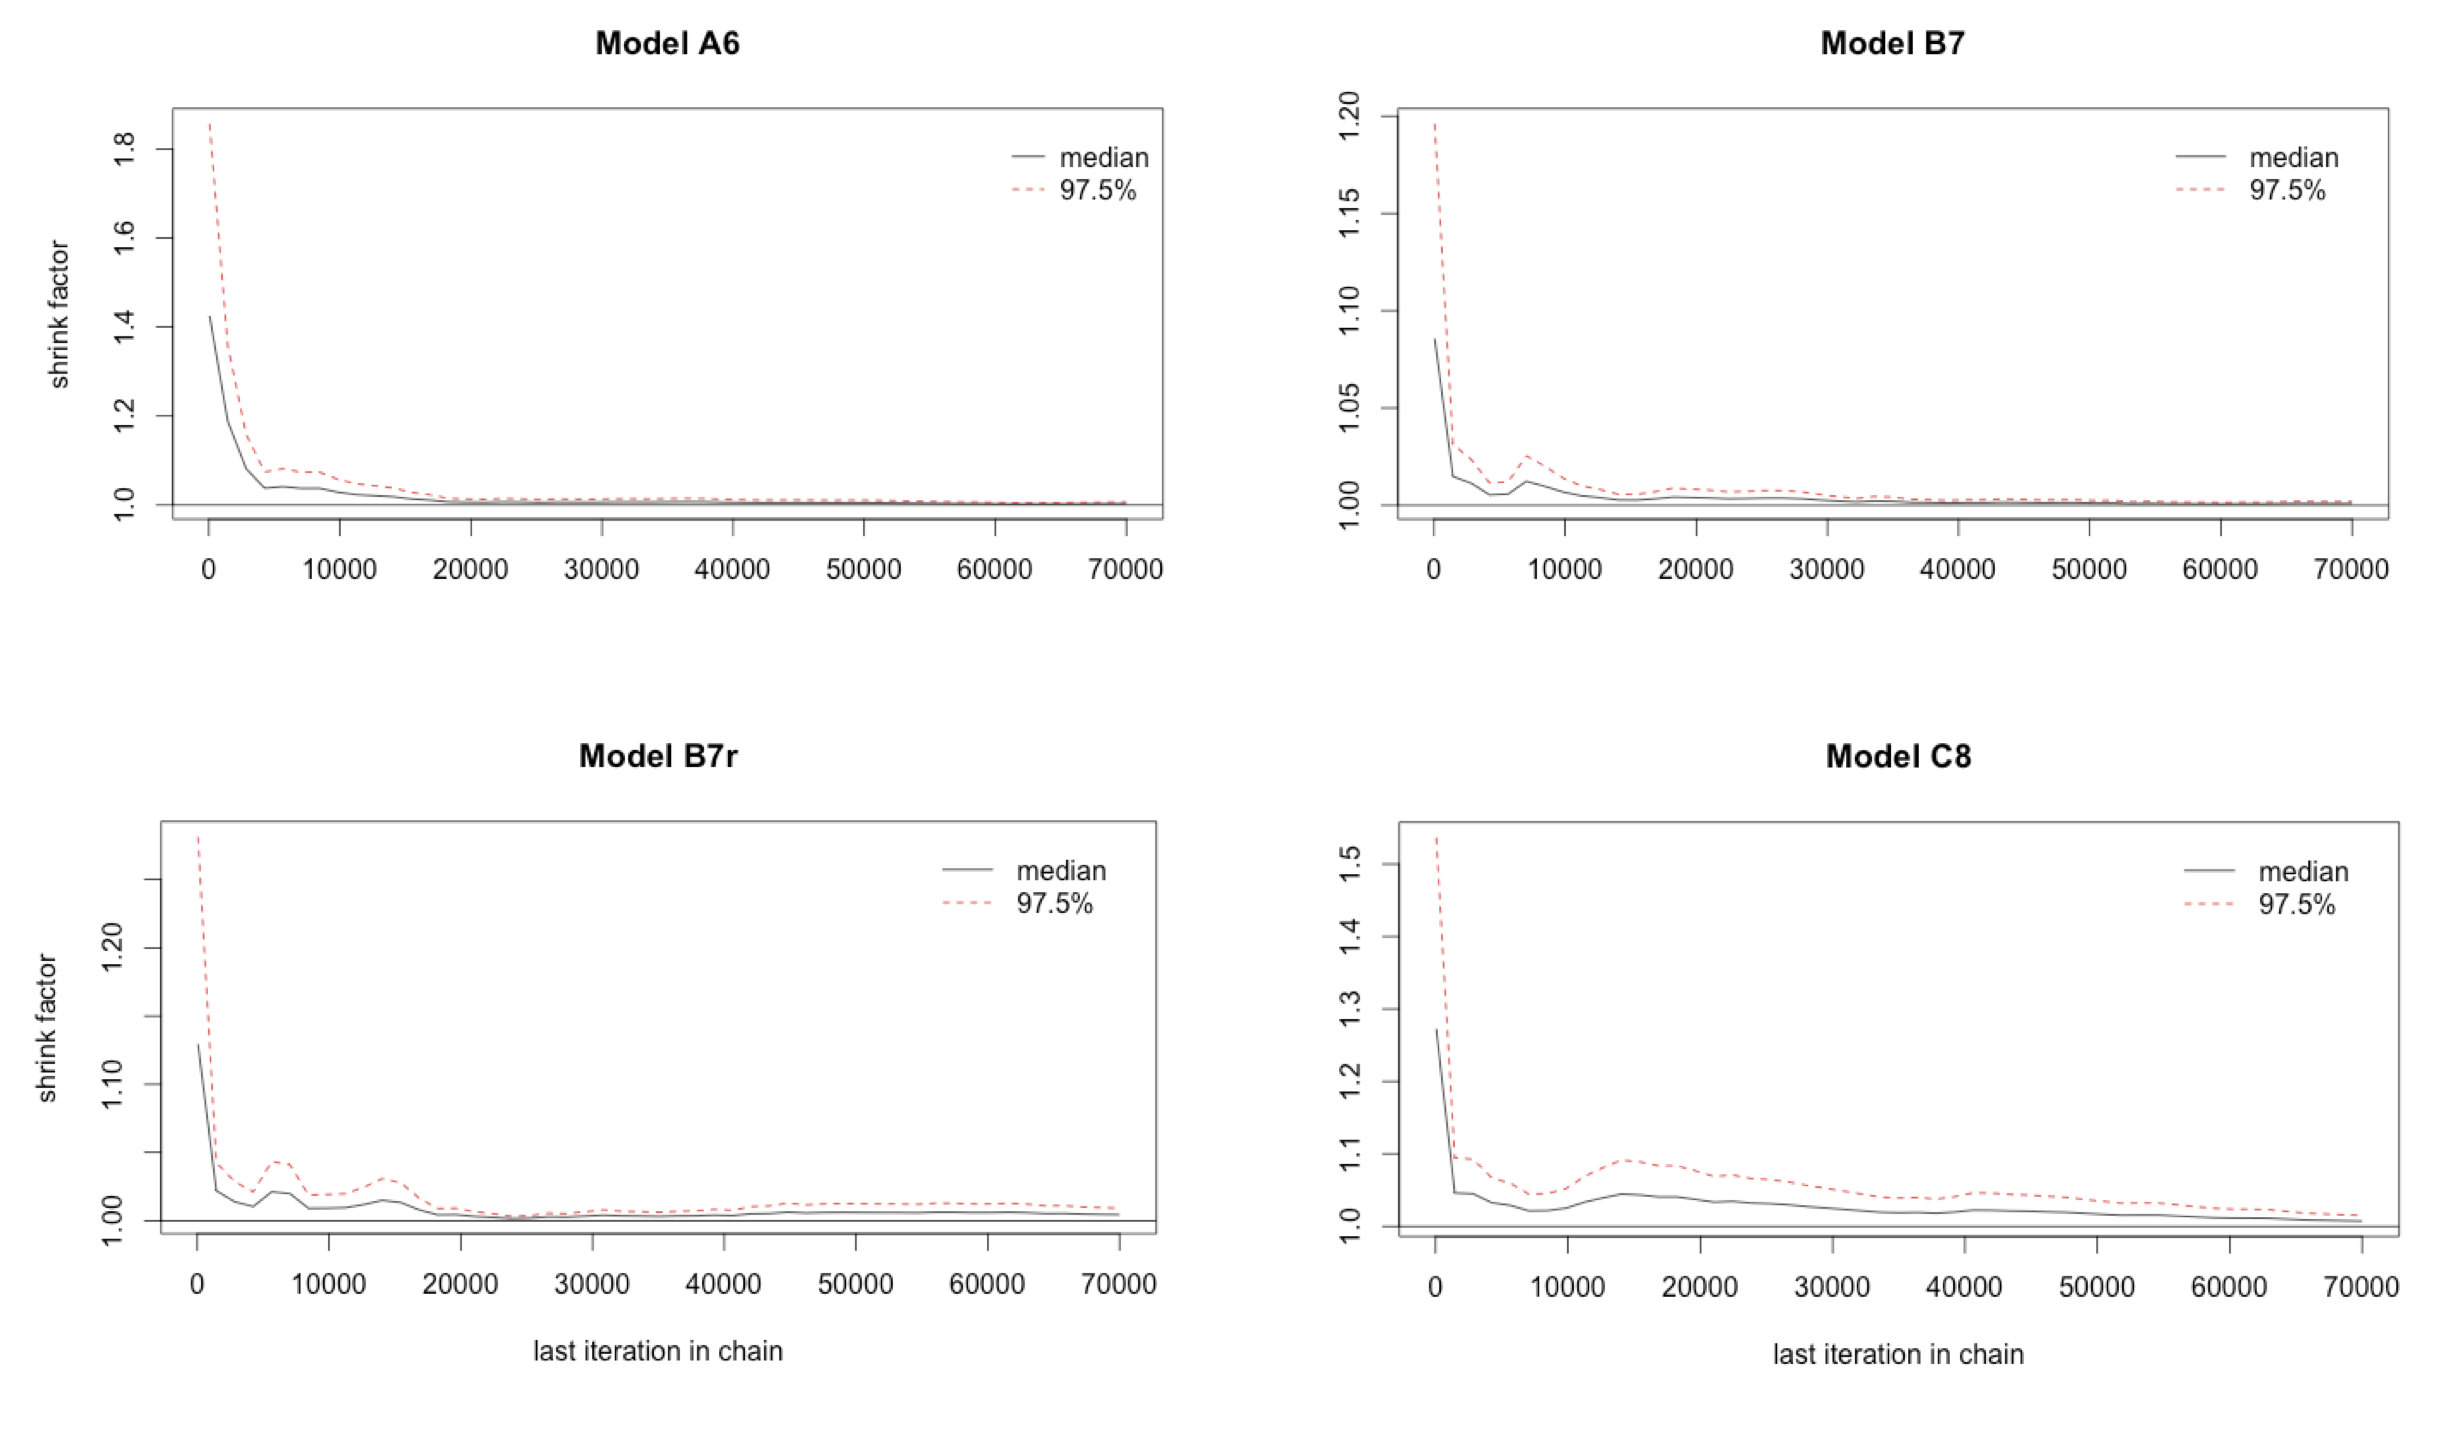
\includegraphics[height = 12cm, width = 13.5cm]{tex/embryo/figure-3.png}
  \caption{MCMC convergence diagnostics: Gelman plot showing the evolution of the gelmna-rubin statistic for four models (A6, B7, B7r, C8) as a function of iterations. The diagnostic metric was evaluated for 10 independent chains with random start points for each model. Values less 1.2 imply good mixing of the chains. Diagnostic plots for other models can be found in Additional File 1.}
\label{fig:figure-3}
\end{figure}




\subsection{Marginal likelihood and Bayes factors}

The output from the PT-MCMC at different temperatures was used for computing the marginal likelihood. For each model, we computed the estimate of the log of the marginal likelihood estimate from 10 parallel runs using thermodynamic integration (see methods). 10 independent runs of the sampler were used to compute the estimate and are shown in fig. \ref{fig:logML}. The estimates show low variability. Based on the log of the marginal likelihood, it is straightforward to compute the Bayes factors (see table \ref{table2} for interpretation of Bayes factors). We find that the Bayes factor for model C8 over model B7 is very strong. However, there isn't strong evidence supporting model D8 over model C8. This leads us to believe that there isn't strong evidence from the data to support Bicoid activation of Kruppel. However, the data does support a different distribution for the node specific parameter describing the binding affinity of Bicoid. This is evidenced by the fact that there isn't strong evidence for model C8 over model B7r. 

\begin{figure}
\centering
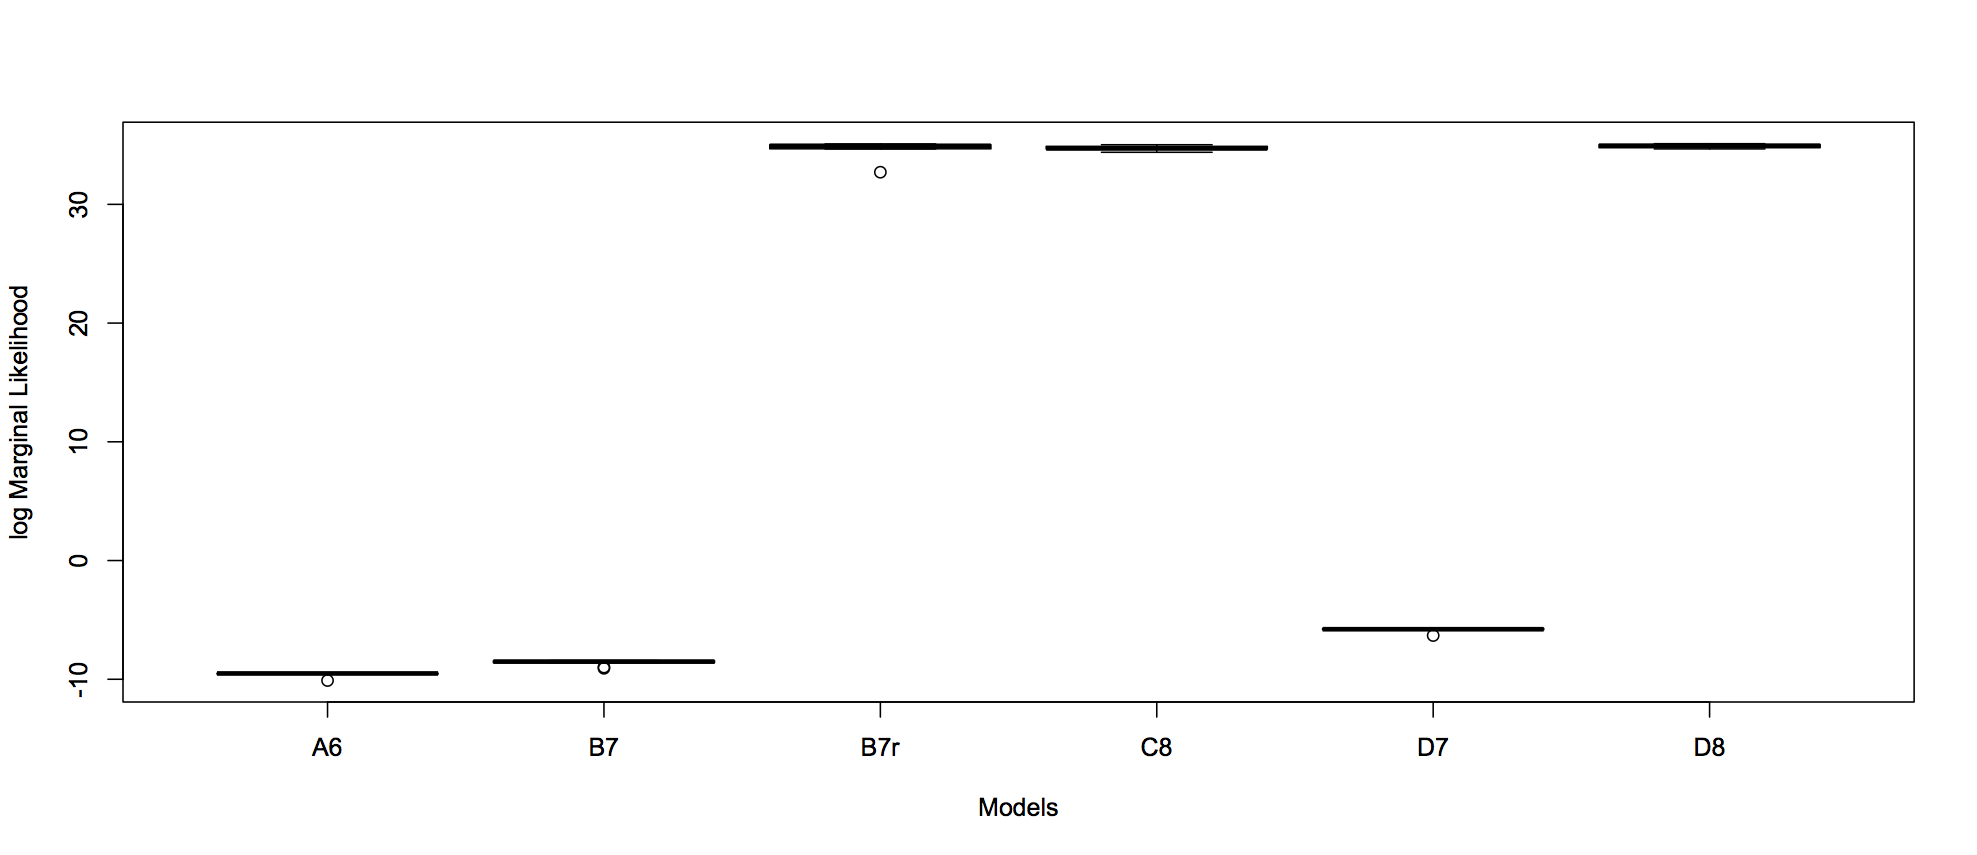
\includegraphics[height = 10cm, width = 10cm]{tex/embryo/figure-4.png}
\caption{Thermodynamic estimate of the logarithm marginal likelihood for all models. Estimates were generated for 10 independent runs for each model and show low variance. Difference between the estimates for models reveals the log Bayes factor that can be used for model comparison (see table \ref{table2}). We see that addition of a node specific-parameter for Bicoid improves the model fit in a statistically significant manner.}
\label{fig:logML}
\end{figure}

%\hl{It might be pertinent here to contrast the model selection approach under the Bayesian paradigm to the model validation approach of cross-validation {\cite{Kohavi95astudy}}. Cross-validation is a popular approach to characterize over-fitting of models to the data. Here, we can envisage, excluding some of the data during model fitting step (validation set) and then testing the accuracy of the model on this held-out data set. However, the process of model selection described here, infact, helps guard against such over-fitting by over-parameterized models by penalizing them implicitly for higher dimensionality. This ability of Bayes factors to guard agianst over-fitting has also been discussed elsewhere {\cite{jeffreys92}\cite{girolami08a}} and offers similar advantages like the cross-validation approach. } 

\begin{table}[h]
\centering
\begin{tabular}{lll}
\hline
$2log_{e}(B)$ & $B$ & Evidence against $H_0$ \\ \hline
0 to 2 & 1 to 3 & Not worth more than a bare mention \\
2 to 6 & 3 to 20 & Substantial                      \\
6 to 10 & 20 to 150 & Strong                      \\
$> 10$ & $> 150$ & Very strong                      \\ \hline
\end{tabular}
\vspace{0.25in}
\caption{Criteria due to Kass \& Rafferty \cite{raftery95} for interpretation of Bayes factor as evidence support categories.}
\label{table2}
\end{table}

\subsection{Gene expression profiles}
Model outcomes were generated by sampling from the joint posterior of the model parameters. For each model, 100 samples were taken from the joint distribution and the model outcomes generated by using the parameter set (see fig. \ref{fig:figure-5}). The basic model with 6 parameters (model A6) also captures the main features of the expression pattern, showing that the inference procedure is able to sample from the correct posterior. As the likelihood is computed only within certain domains (shown by vertical dotted lines for each gap gene in fig. \ref{fig:figure-5}), model outcomes show higher variability outside these domains. Most noticeable is the posterior shift of Hunchback expression seen in models B7r and C8. This shows that a different distribution of Bicoid binding affinity from the global affinity parameter is sufficient to capture the characteristic expression curve of Hunchback. Increasing the number of parameters from 7 to 8 improves the model fit (as judged from the marginal likelihood), it does so not in a statistically significant manner. The model outcomes for models D7 \& D8, that describe models with an extra regulatory edge for Bicoid, can be found in fig. \ref{fig:model-predictions-d7-d8}. 

\begin{figure}[h!]
\centering
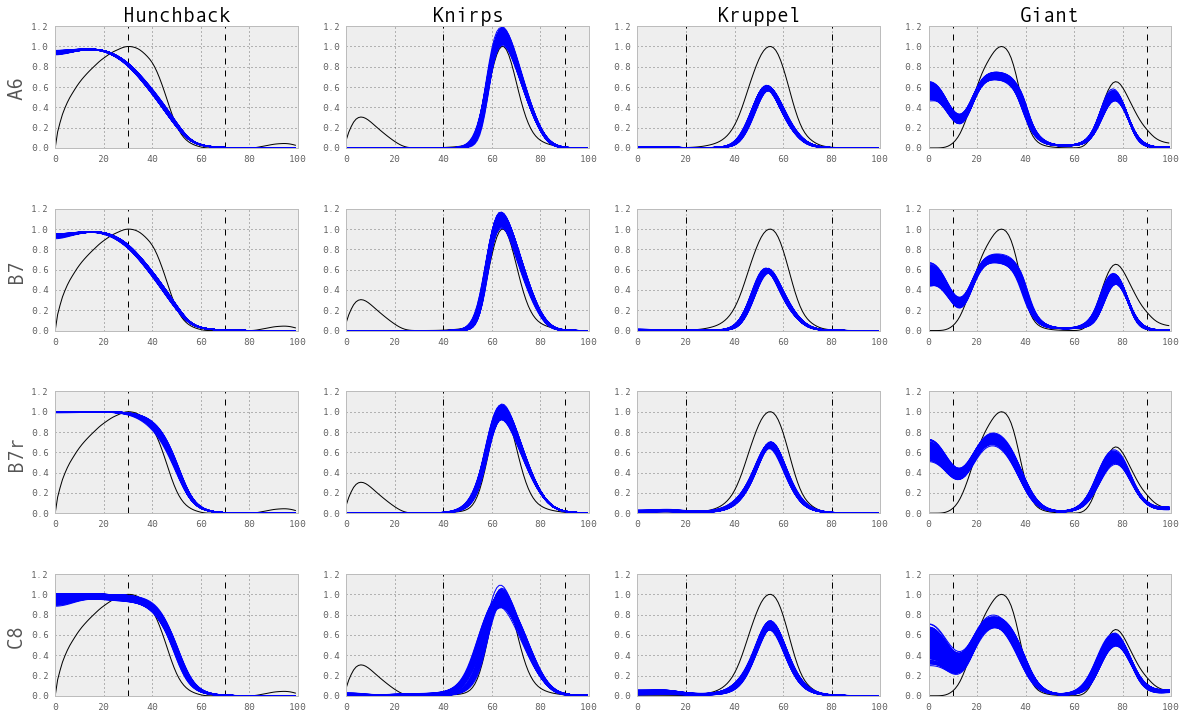
\includegraphics[height = 10cm, width = 12.5cm]{embryo/figure-5.png}
\caption{Gene expression profiles for Models A6, B7, B7r, C8. Black lines show observed values and blue lines are model outcomes by sampling parameters from the joint posterior. For each model, 100 samples were drawn from the joint posterior of model parameters. Vertical dotted lines show domains over which the likelihood was computed.}
\label{fig:figure-5}
\end{figure}

\begin{figure}[h!]
\centering
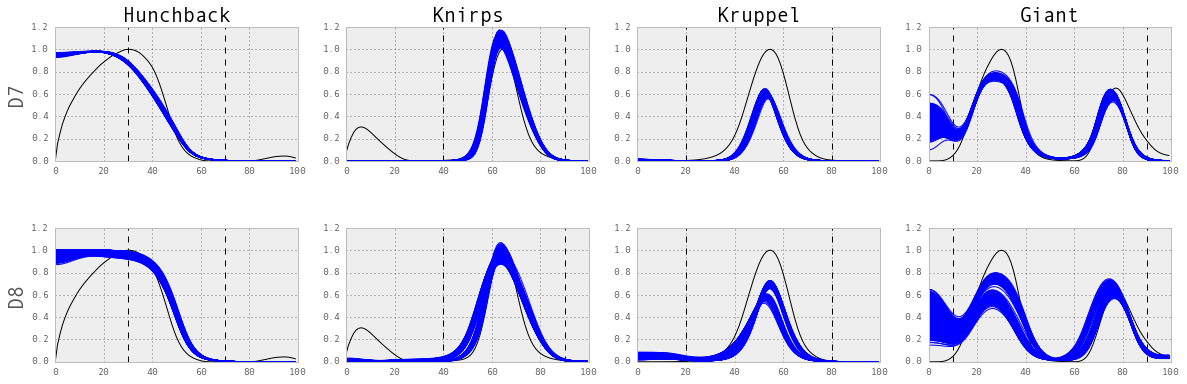
\includegraphics[height = 8cm, width = 12.5cm]{embryo/model-predictions-d7-d8.png}
\caption{Gene Expression profiles for models D7, D8. Black lines show observed values and blue lines are model outcomes by sampling parameters from the joint posterior. For each model, 100 samples were drawn. Vertical dotted lines show domains over which the likelihood was computed.}
\label{fig:model-predictions-d7-d8}
\end{figure}

\subsection{Over-fitting analysis}
We tested the best performing model (according to Bayes factor criteria), model B7r, for over-fitting. We used a modified cross-validation (CV) approach for testing over-fitting (see methods). In each CV-fold, we fit the model to the training set and then draw 100 samples from the posterior parameter distribution. The posterior samples are used to predict values for the held out set. We use the mean log-likelihood metric as prediction accuracy measure. As a Gaussian error model is used, the mean log-likelihood is proportional to the residual error in this case.  The mean log-likelihood for the cross validation set is 0.314 ($\pm$ 0.024). The mean log-likelihood using samples from posterior parameter distribution generated using the complete data is 0.326 ($\pm$ 0.061). Using a Student's t-test with Welch modification, we found the difference in means to not be statistically significant ($P > 0.05$) indicating that the model doesn't over-fit the data.

\section{Conclusions}

Recovering gene regulatory network information from expression data is a key problem in systems biology. Particularly in the study of the segmentation pathway for early \textit{Drosophila} embryo, various modeling approaches have been taken \cite{jaeger04b, jaeger06b, papatsenko11}. However, most of these modeling approaches rely on the assessment of a single candidate model. This sort of approach has been previously argued against \cite{chamberlin1890} as it doesn't pay heed to competing hypotheses and hence, other plausible explanations. In addition, inference in these approaches rely on optimization techniques which do not account for uncertainty in experimental measurements. Optimization approaches try to offer measures of parameter certainty through sensitivity analysis but, barring certain studies \cite{Rodriguez13}, the issue of comparing models has been largely unaddressed. 

We do note that there have been some attempts \cite{odell00} at doing model selection in the \textit{Drosophila} embryo. However, the application of a structured framework in which models can be compared is still elusive. Doing the analysis in a Bayesian framework provides a more standard procedure to address both the issues of performing inference regarding different models and to assess the uncertainty of parameter estimates. An important issue when working with dynamical models is the issue of identifiability \cite{Raue14, Oana11, Villaverde16, Becker13} - the ability to unqiuely estimate parameters of the model given the data. In the Bayesian context, \textit{a priori} identifiability issues can be detected by examining the covariance structure of the full parameter posterior distribution. Parameters that are confounded will be tightly correlated. Identifiability issues can be surmounted by providing a more informative prior that more tightly constrains confounded parameters. In our case, however, we have chosen to work with uniform priors to indicate that our knowledge of the system is still evolving. Indeterminacy of model parameters are incorporated into the marginal likelihood, allowing one to still perform model selection. However, parameter relationships can still uncover important mechanisms. In our study, we find that the parameters for binding affinity and number of sites are negatively correlated (fig. \ref{fig:corner}). Such a relationship is expected as it indicates that a transcription factor can modulate gene expression by either binding strongly to a few sites or through weak binding to multiple sites. Similar to our study, Chertkova \emph{et al.} \cite{Chertkova2017}, show that loss of transcription factor binding sites in \emph{in silico} models results in increase in binding affinity of transcription factors, supporting negative correlation between these parameters in order to maintain gene expression. 

In the Bayesian framework, Bayes factors provide a means of doing model selection and have been employed to compare between ODE based models \cite{calderhead10, girolami08b, schmidl12, lygeros10}. We show here that similar approaches can be used for doing model selection in the context of PDE models for spatial patterning. An advantage of the Bayesian model selection paradigm using Bayes factors is that it doesn't require models to be nested, i.e models need not follow a set hierarchy where all models may be derived from an extended parameterized model. This particularly advantageous when we attempt to test hypotheses involving different network topologies. Samples from the posterior of parameter distribution were generated using the parallel tempering (PT-MCMC) sampler. This sampling approach can be easily combined with the numerically stable thermodynamic integration method to estimate marginal likelihood for each of the competing models. These estimates in turn can be used to compute Bayes factors. Our analysis shows that besides the global binding affinity parameter, a different node-specific parameter is required for describing the regulatory effect of Bicoid on its target genes. This may point to the fact that the molecular mechanism of activation by Bicoid is different from other maternal/gap genes. The node-specific Bicoid binding affinity parameter helps account for a posterior shift of Hunchback expression. A candidate hypothesis for the activation of Kruppel by Bicoid was also tested for. Our analysis offers little support for the activation of Kruppel by Bicoid. 

Our study seeks to provide a statistical framework in which predicted expreimental hypothesis can be tested. In addition, the model selection procedure also ensures that a minimal model for gap gene expression can be formulated. 

We point out that as the computation of posterior probabilities in Bayesian analysis involves integration over high-dimensional parameter spaces, sampling from higher dimensions becomes increasingly difficult. This is a particular limitation for the large parameter models that we see in systems biology. While there has been some progress in Bayesian parameter estimation in high-dimensions \cite{theis13}, this problem is far from solved. However, there might be some justification in criticism that these high-dimension models also tend to be over-parameterized and thus too flexible. One approach would be do a hierarchical Bayesian analysis \cite{Carlin_Empirical_2000} to constrain parameter sets in order to prevent the problem of over-fitting and estimation in higher dimensions. 

% chickpea
\chapter{Nested association mapping analysis for chickpea hybrids}
\label{cha:research_topic_2}

\section{Introduction}

Cultivated chickpea (\textit{C. arietinum}), a small herbaceous plant, is the world's second most important pulse legume and is one of the earliest cultivated legumes \cite{vonWettberg2018, Sani2018}, with particular importance in the semi-arid tropics of sub-Saharan Africa and South Asia. Domesticated chickpea is believed to have diverged from its closest wild relative \textit{C. reticulatum} (fig. \ref{fig:cicer-phylo}) around 10,000 years ago \cite{vonWettberg2018}. 

\begin{figure}[h!]
    \centering
    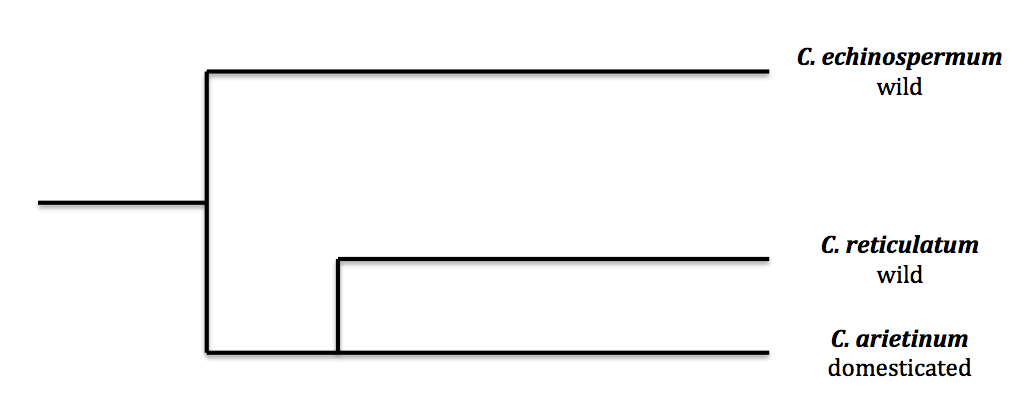
\includegraphics[scale=0.8]{tex/chickpea/chickpea.png}
    \caption{Phylogenetic relationships in chickpea (\textit{cicer}).}
    \label{fig:cicer-phylo}
\end{figure}


The process of domestication and breeding has unintended consequences for a species. The nature and 
intensity of artificial selection imposed by breeders can impart genetic drift, reduce diversity and increase the frequency of deleterious alleles. This reduced diversity and fixation of deleterious alleles has varied implications - it constrains our ability to expand the cultivation of crops into environments that differ from those under which domestication occurred and the reduced diversity makes the crop susceptible to  changing climate and pathogens. Indeed, in the case of the cultivated banana which is clonally propagated with extremely low diversity, the entire crop variety, \emph{Gros Michel}, has been wiped out by the Panama disease \cite{Ordonez2015}. A second wave of the Panama disease, similarly, threatens to wipe out the present \emph{Cavendish} banana variety \cite{Ordonez2015}. 

Domesticated chickpea has undergone an extreme domestication-related genetic bottleneck \cite{vonWettberg2018}. This has consequences for breeding of climate-resilient crop varieties, because much of the historical phenotypic plasticity necessary to tolerate environmental extremes may have been lost through domestication. Breeding only within cultivated material will have steeply diminishing returns, and there is an urgent need for new sources of diversity, for example, from wild material \cite{McCouch2013, Dempewolf2014, Hajjar2007}.

Sampling wild populations to make a genetic resource for the breeding community requires a consortium level effort. Keeping this goal in mind, the `Feed the Future Innovation Lab for Chickpea' was formed and has the objective of comprehensively characterizing a collection of wild species focused on \emph{C. reticulatum}, the wild progenitor of cultivated chickpea. Concurrently, we wish to develop a predictive network of genotype-phenotype associations that identifies genes and genome regions from wild species that improve chickpea's yield resilience to climatic extremes and helps bring back some of the lost diversity in to cultivated chickpea. 

Such programs have been carried out with great success in maize \cite{McMullen2009}, soybean \cite{Bandillo2017} and various other crops. Traditionally, linkage analysis, where crosses (back-cross or inter-cross generation) between two parents are made, has been used for the identification of genomic regions of interest affecting a particular phenotype. This approach relies on recent recombination and generally suffers from low resolution as the linkage blocks tend to be very large. Additionally, as we sample alleles from only two parents, there is low allelic richness in such mapping populations. A competing approach would be to sample populations from natural populations and rely on ancestral recombination. This approach has much better resolution but suffers from statistical power as the causative allele might be at low frequency in the population, requiring a large sample size to detect it. To alleviate concerns in both these approaches while still retaining the advantages of both, it was suggested to make a nested association mapping (NAM) \cite{McMullen2009} population for association mapping. 

In NAM populations, several founders (wild individuals) are crossed individually with a common cultivated parent. The F1 progeny are then selfed for a number of generations to produce recombinant inbred lines. %(fig. \ref{fig:nams}) 
NAM take advantage of both historic and recent recombination events and have advantages of low marker density requirements, high allele richness, high mapping resolution, and high statistical power \cite{Yu2008, McMullen2009}. 

%\begin{figure}
%    \centering
%    \includegraphics{}
%    \caption{Process of creating NAM populations}
%    \label{fig:nams}
%\end{figure}

In this chapter, we describe the NAM population developed for identifying genetic basis of agronomic traits in chickpea. A summary of the phenotypic distributions seen in the hybrids is also provided. We then assess how much of the variation can be attributed to additive and dominant effects. Lastly, we use a linear model to map the phenotypes onto genotypic data. 

\section{Materials and methods}

\subsection{Genotype and phenotype data}

19 diverse chickpea lines were chosen as the parental lines (fig. \ref{fig:wild-parent}) for the NAM population in order to encompass the remarkable diversity of chickpea and preserve historic linkage disequilibrium. Each parental line was crossed to the cultivar ICCV96029 (chosen as a reference line due to its wide deployment as one of the most successful commercial lines) to create the F1 population. The F1 plants were then self-fertilized for one generation in order to create a total of around 100 F2s per family, for a total of 2139 F2s within the NAM population (fig. \ref{fig:crosses}).

Each cross was then sequenced using genotype-by-sequencing \cite{He2014} techonology. Genotyping-by-sequencing offers a rapid and cost-effective means to identify genome-wide nucleotide variation in crop germplasm. The NAM lines were sequenced to a coverage of around 5X and aligend to the 2013 chickpea reference \cite{Varshney2013}. The shallow coverage led to an over-representation of homozygous calls. TASSEL's FSFHap algorithm \cite{Swarts2014}, was used to correct variant calls in the sequenced lines. To assess problems with the called genotypes, one of the cross families (ICCV96029 x Besev\textunderscore079) was analysed for recombination events. Fig. \ref{fig:unimputed-res} shows the number of recombination events (REs) per site as assessed by a change in phase (from homozygous wild, homozygous cultivated or heterozygous to another state) along the genome. As we can see, for a family size of 80 individuals, almost half the indidividuals show an RE. This is contrary to what is expected. Fig. \ref{fig:imputed-res} shows a similar plot but after imputation. As we can see, the number of REs per site has gone down significantly. There remain peaks where the REs per site are very high. We think that these regions reflect problems with the 2013 draft and are essentially misassembled regions that the imputation algorithm cannot fix. 

\begin{figure}
    \centering
    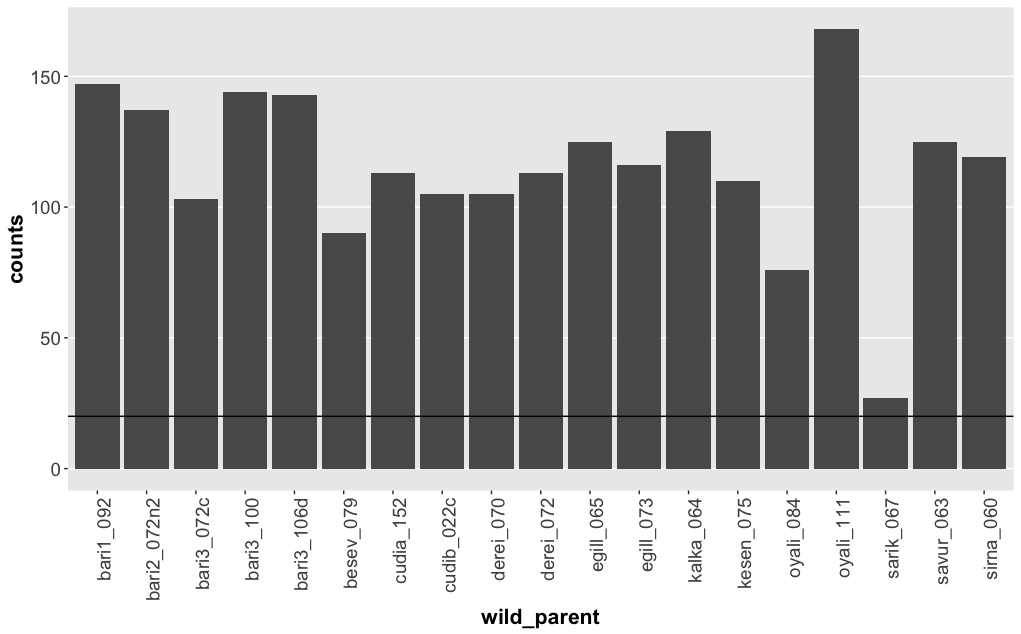
\includegraphics[scale = 0.4]{tex/chickpea/wild_parent.jpeg}
    \caption{Chickpea wild parents sampled from diverse regions in Turkey. X-axis shows the name of each founder and Y-axis represents the number of times the line participated in a cross.}
    \label{fig:wild-parent}
\end{figure}

\begin{figure}
    \centering
    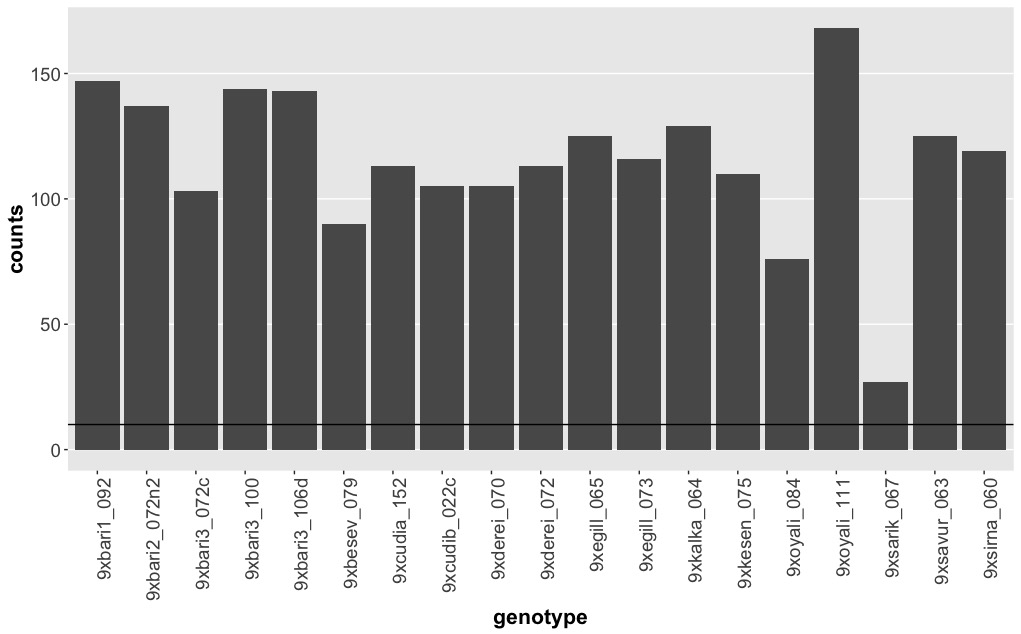
\includegraphics[scale=0.4]{tex/chickpea/crosses.jpeg}
    \caption{NAM crosses. X-axis represents the cross name and y-axis is the number of individuals in a particular family.}
    \label{fig:crosses}
\end{figure}

\begin{figure}
    \centering
    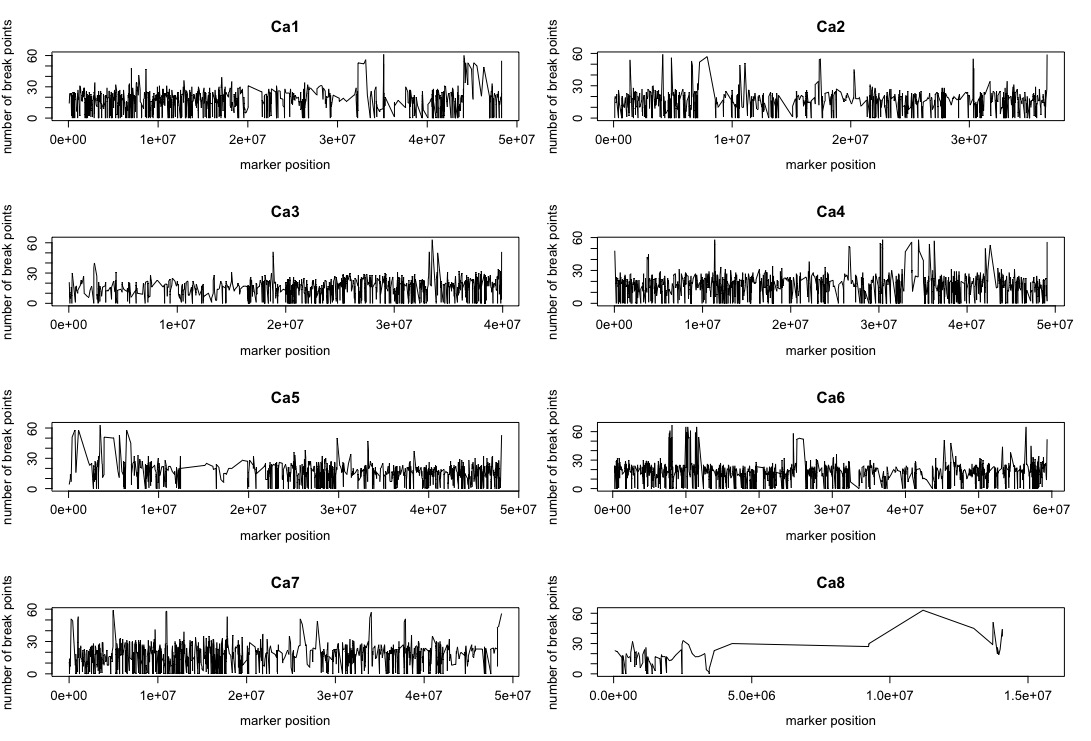
\includegraphics[height = 15cm, width = 15cm]{tex/chickpea/unimputed-res.jpeg}
    \caption{Recombination events along the chromosome for unimputed data for the ICCV96029 and Besev\textunderscore079 cross. Nearly half the individuals show a recombination each position, indicating that the gentoypic data is very noisy. The expected number of recombinations is extremely low as we deal with an F2 cross. X-axis: marker position (in bps). Y-axis: number of break points.}
    \label{fig:unimputed-res}
\end{figure}

\begin{figure}
    \centering
    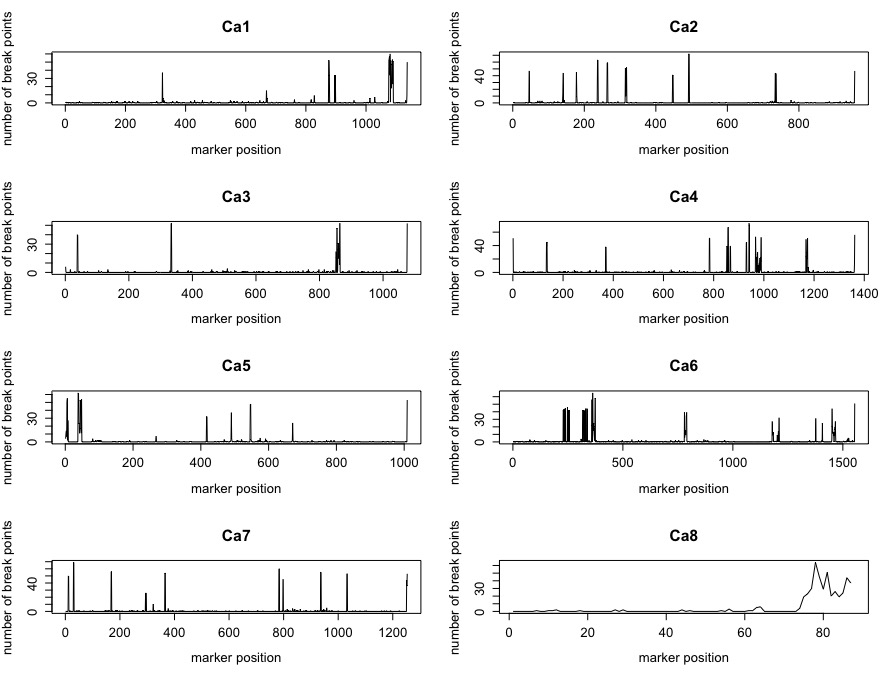
\includegraphics[height = 15cm, width = 15cm]{tex/chickpea/imputed-res.jpeg}
    \caption{Similar to fig. \ref{fig:unimputed-res} but now plotted with imputed data. The number of REs has dropped significantly except for certain regions. These regions could not be corrected by the algorithm and were particularly noisy. We believe they might represent problematic regions with the reference draft.}
    \label{fig:imputed-res}
\end{figure}

The F2s were grown using a common garden design and several phenotypes were collected. We selected 6 agronomically relevant phenotypes for this study that are listed below:

\begin{enumerate}
    \item \textbf{Total plant biomass}: total mass of the plant
    \item \textbf{Plant volume}: total volume of the plant; measured by immersing plant in water
    \item \textbf{Average mass of seed}: total mass of seeds divided by the total number of seeds
    \item \textbf{Yield}: total mass of seeds
    \item \textbf{Harvest index}: total mass of seeds as a percentage of the total above ground mass of plant
    \item \textbf{Shattering index}: total number of seeds that are shattered (dispersed) as a percentage of the total number of seeds
\end{enumerate}

\subsection{Marker selection}

The markers selection was done based on two criteria.
\begin{enumerate}
    \item For the segregation distortion analysis, the variants were filtered for 1\% minor allele frequency
    \item For the association mapping analysis, the markers were first separately filtered for intermediate frequency (35\%) by family. The markers were then imputed to correct for erroneous calls and then all the markers across families were combined together. The combined set was filtered for a missingness rate of 20\%. The combined set was then used for association mapping. 
\end{enumerate}
Fig. \ref{fig:marker-by-length} shows the number of markers versus the length of the chromosome. We see that chromosome 8, the smallest chromosome, has the least number of markers. Besides the length, chromosome 8 also suffers from distortion, thus, most of the markers do not meet the intermediate frequency requirement. 

\begin{figure}
    \centering
    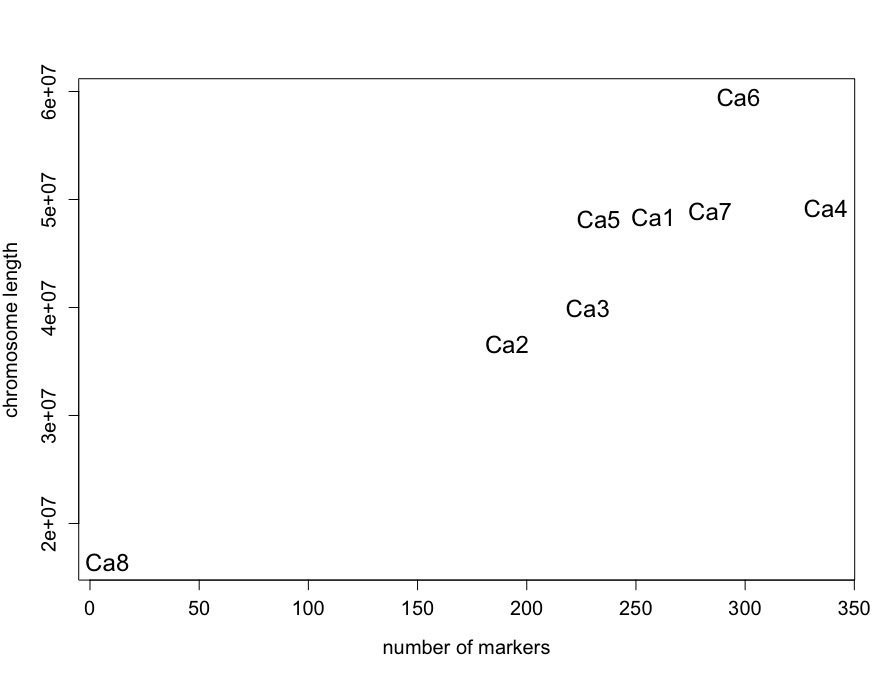
\includegraphics[scale = 0.45]{tex/chickpea/marker-by-length.jpeg}
    \caption{Number of markers (x-axis) used for association mapping analysis versus the length of the chromosome (y-axis) }
    \label{fig:marker-by-length}
\end{figure}

\subsection{Mixed models and heritability estimates}

Linear mixed models (LMMs) describe the outcome variable $Y$ as a linear combination of deterministic (fixed) effects and random effects. Random effect is the realization of a random variable whose distribution we try to model:

$$Y = \underbrace{X\beta}_{fixed\ effects} + \underbrace{Zb}_{random\ effects} + \underbrace{\epsilon}_{noise}.$$

LMMs can be used for heritability estimation in genetic analysis of plant and animal breeding \cite{Ogunniyan2014,Valdar2006}. We can consider all the markers for together as random effects in a genotypic model:

$$Y = X\beta + \sum_{i=1}^{m}W_ia_i + \sum_{i=1}^{m}Z_id_i + \epsilon,$$
where $Y$ is the outcome variable, $X$ is the design matrix for co-variates, $W_i$ accounts for the additive allele coding of the wild allele and $Z_i$ accounts for the dominance allele coding, $\epsilon$ is the unmodeled noise. The coefficients $\beta$, $a_i$ and $d_i$, account for the co-variate (fixed), additive (random effects) and dominance (random effects) deviation respectively. We assume that $a_i \sim N(0, \frac{\sigma^2_a}{m})$ and $d_i \sim N(0, \frac{\sigma^2_d}{m})$ where $\sigma_a^2$ and $\sigma_d^2$ is the additive and dominance variation explained jointly by all, $m$, markers. The noise term $\epsilon$ is meant to represent environmental noise and is assumed to be distributed as $N(0, \sigma_e^2)$. We argue that since we use all the markers together, we are able to tag all of the causal variants from observed SNPs. In this way, we can write:

$$\hat{h}^2_a = \frac{\hat{\sigma}_a^2}{var(X\beta) + \hat{\sigma}_a^2 + \hat{\sigma}_d^2 + \hat{\sigma}^2_e}$$ and, 
$$\hat{h}^2_d = \frac{\hat{\sigma}_d^2}{var(X\beta) + \hat{\sigma}_a^2 + \hat{\sigma}_d^2 + \hat{\sigma}^2_e},$$

where $\hat{h}^2_a$ and $\hat{h}^2_d$ are the additive and dominance estimates of heritability \cite{Da2014}. We also caveat that as a consequence of incomplete and uneven tagging of causal variants from the observed SNPs, this model will give lower heritability estimates compared to the ideal model.

\subsection{Association mapping approach}

We map the effect of each marker as a linear model. The first 8 principal components are used to correct for relationship between the founders. In addition, we use a genotypic model and adjust for group effects. A genotypic model accounts for both additive and dominance effects in the model. The model takes the form:
$$Y = X\beta + Wa + Zd + \epsilon,$$
where $Y$ is the outcome variable, $X$ is the design matrix for PC co-variates and group means, W accounts for the additive allele coding of the wild allele and Z accounts for the dominance allele coding, $\epsilon$ is the unmodeled noise. Throughout, at each marker, we choose the additive coding `0-1-2' where each count represents the wild allele and the dominant coding `0-1-0' where 1 indicates the heterozygous state. The coefficients $\beta$, $a$ and $d$, account for the co-variate, additive and dominance deviation respectively. 

Based on the estimates of the additive effect ($a$) and dominance deviation ($d$), we can ascertain dominance conditions at a locus, thus, 
\begin{itemize}
    \item \textbf{co-dominance}: $d = a$
    \item \textbf{over-dominance}: $d > a$
    \item \textbf{under-dominance}: $d < a$
\end{itemize}

We remark that the advantage of the so-called `genotypic' model used here is that it helps us identify the type of dominance at a locus without using a separate model for dominance. The linear models were fit using the plink \cite{Purcell2007} software. 

\section{Results}


\subsection{Segregation distortion}
In  cross species hybrids, incompatibilities can occur due to viability selection at a locus \cite{McMullen2009, Zhan2011}. Such a selection will cause `distortion' or deviation from Mendelian segregation ratio at a linked marker. One approach to visualize distortion loci is to look at proportion of either parent at a marker. The expected frequency of either parent should be around 50\% and extreme deviation from this proportion point to distortions in the hybrids. Fig. \ref{fig:seg-dis} show the distortion within NAM families. We see that chromosome 8 is heavily distorted towards the cultivated allele. Additionally, several NAM families show a distortion towards the wild allele on chromosome 5. 

\begin{figure}
    \centering
    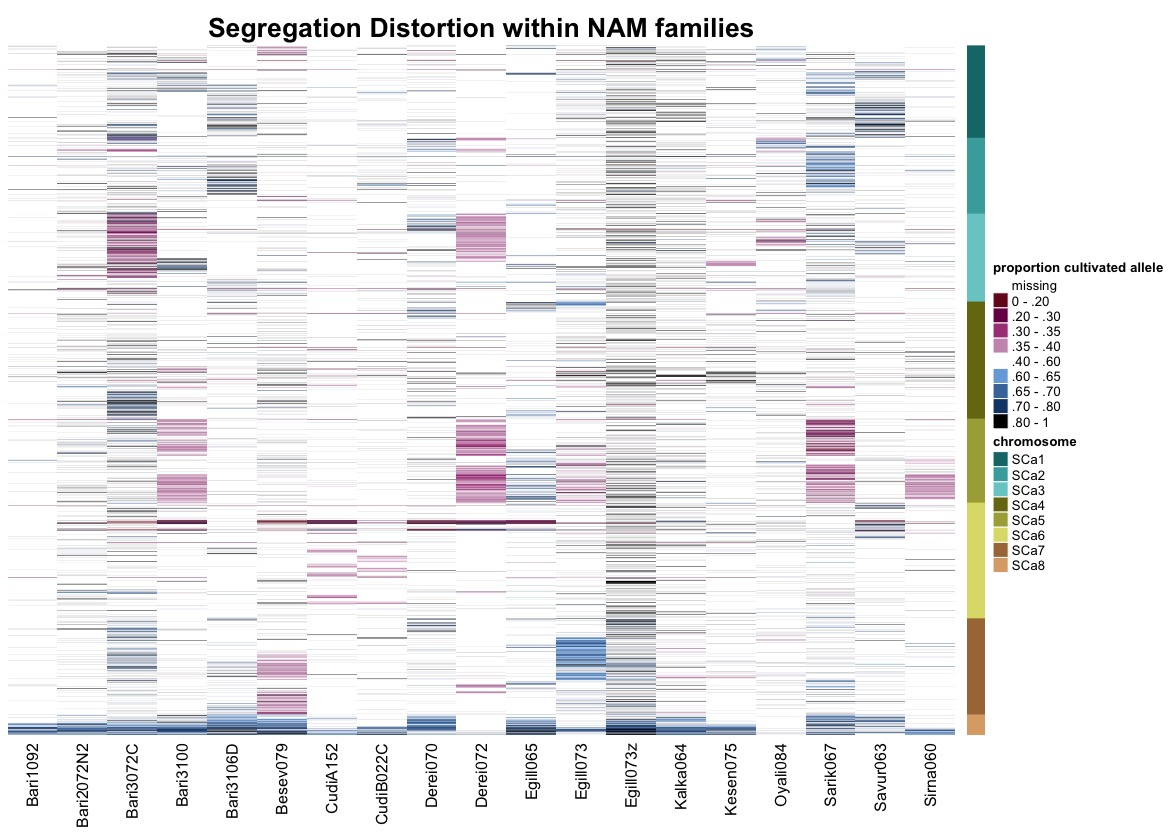
\includegraphics[height = 15cm, width = 15cm]{tex/chickpea/Segdis.jpeg}
    \caption{ Segregation distortion within individual NAM families. Each column represents one NAM family, the wild parent is indicated below the column. Horizontal lines indicate the positions of chromosome boundaries for chromosomes 1 to 10, top to bottom. The proportion of cultivated (ICCV96029) allele for an interval is indicated by the color scale. Chromosome are represented by vertical colour bar.}
    \label{fig:seg-dis}
\end{figure}

\subsection{Phenotypic distributions}
Fig. \ref{fig:pop-dist} seeks to describe family-wise distribution. We see that most of the phenotypes have similar distributions across populations. However, we have some low individuals with low harvest index in the Derei and Sirna families - which concurrently show distortions towards wild allele in fig. \ref{fig:seg-dis}. Low harvest index usually translates to large plants with low fertility and such individuals are good candidates for investigating incompatibility loci. 

Fig. \ref{fig:pheno-corr} looks at phenotypic correlation and distribution of phenotypes across all hybrid families. We can see that most phenotypes are near normally distributed except for shatterring index which we believe to be a more simple trait regulated from a few loci. Perhaps unsurprisingly, many phenotypes show correlation with yield being strongly correlated with `harvest index' and `total plant biomass'. `Plant volume' and `total plant biomass' are similarly correlated. 

\begin{figure}
    \centering
    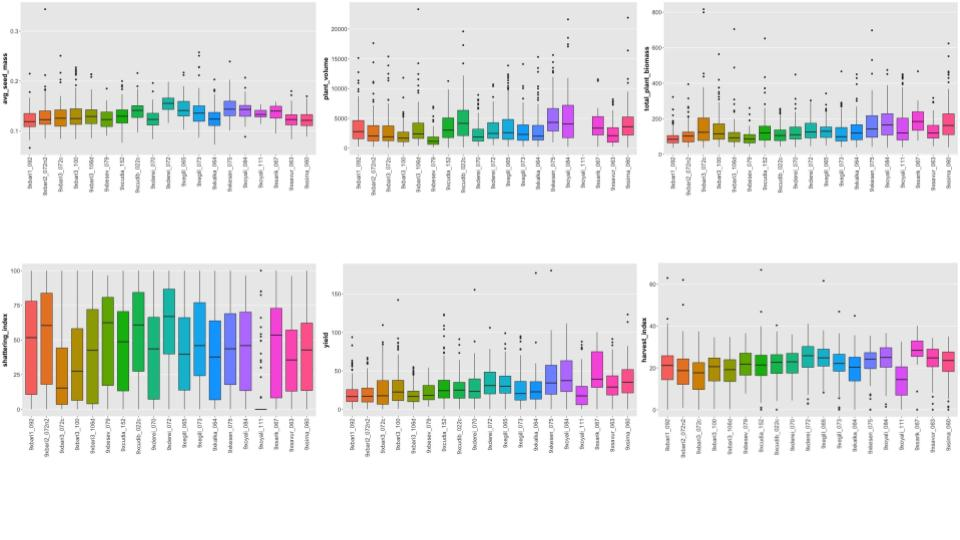
\includegraphics[height = 15cm, width = 15cm]{tex/chickpea/pop-wise-dist.jpg}
    \caption{Population wise distribution of phenotypes. In clockwise order, average seed mass, plant volume, total plant biomass, harvest index, yield and shattering index. X-axis labels indicated the founder that the cultivar was crossed with.}
    \label{fig:pop-dist}
\end{figure}

\begin{figure}
    \centering
    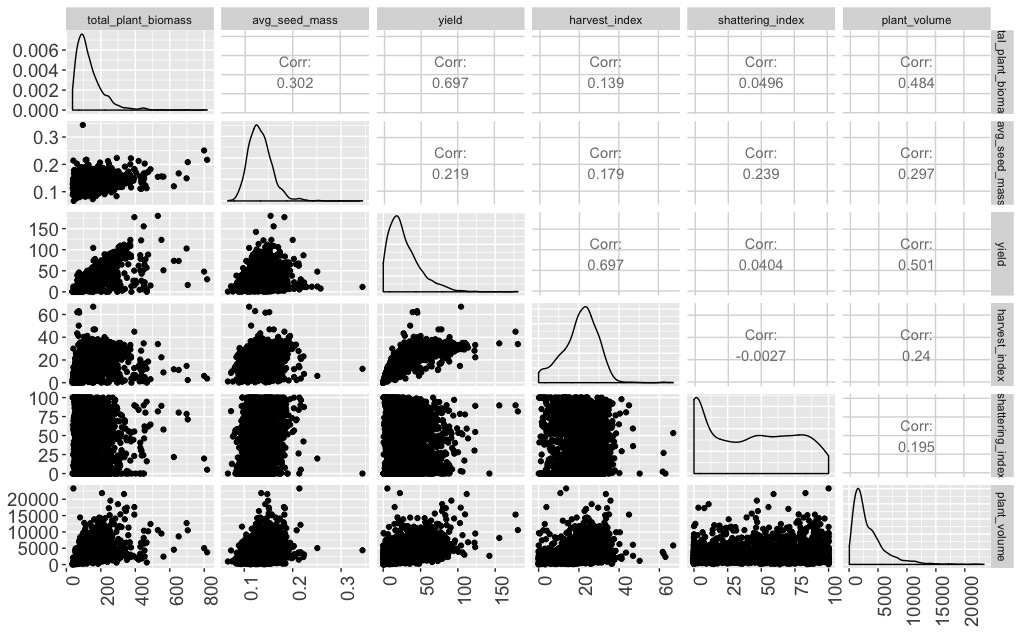
\includegraphics[height = 15cm, width = 15cm]{tex/chickpea/pheno_correlation.jpeg}
    \caption{Phenotypic distribution and correlation across all hybrids. we see that yield is correlated with `harvest index' and `total plant biomass'. Most phenotypes have normal distribution. }
    \label{fig:pheno-corr}
\end{figure}

\subsection{Heritability estimation}

We used GVCBLUP \cite{Wang2014} implementation of the mixed models approach to estimate the additive and dominance contribution to phenotypic variation in the hybrids. As we can see in fig. \ref{fig:varcomp}, the additive contribution is highest for `average seed mass'. This is unsurprising, because most of the selection that has happened in domesticated chickpea is to increase seed size.  A phenotype that has been selected against is shattering, and so perhaps expectedly it too has a strong additive component. We notice that shattering has a very strong dominance component as well, while the other phenotypes show low dominance contributions. 

\begin{figure}
    \centering
    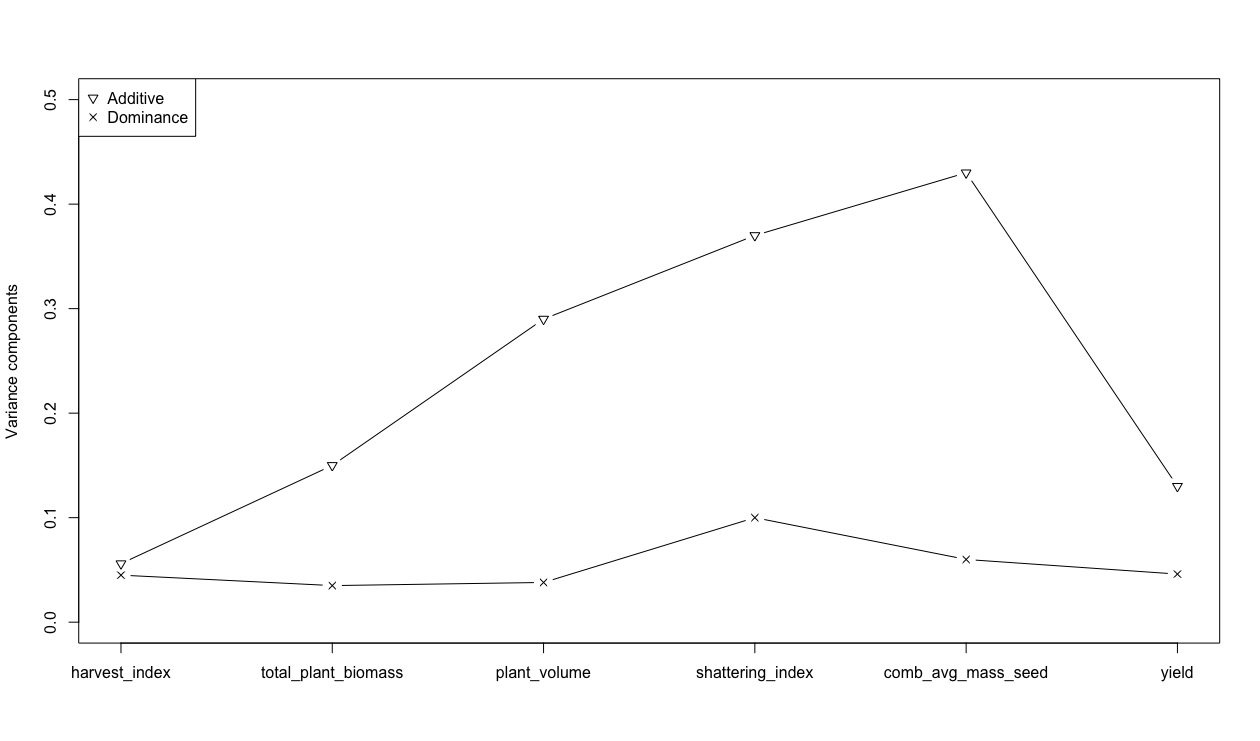
\includegraphics[height = 15cm, width = 15cm]{tex/chickpea/varcomp.jpeg}
    \caption{Additive and dominance variance component estimates of hybrid phenotypes.}
    \label{fig:varcomp}
\end{figure}

\subsection{Single marker analysis}

Finally, we fitted a liner model in which each marker is tested individually for association with the phenotype. As we use a genotypic model, we can tease out additive and dominace deviation effects at each locus. The results for additive effect is presented in fig. \ref{fig:man-add}, for positive dominance in fig. \ref{fig:man-dom} and for over-dominance in fig. \ref{fig:man-over}. 

We see a strong signal for additive effect for shattering on chromosome 6 and chromosome 7. The wild allele in both cases increases the phenotype. Importantly, the wild allele is dominant at chromosome 6 while the locus on chromosome 7 does not seem to have a dominant effect. 

We find significant hits for additive effect for average seed mass, plant volume and plant biomass. However, as expected from the dominance heritability estimates, besides shattering index most phenotypes do not show significance for dominance effect. 

\begin{figure}
    \centering
    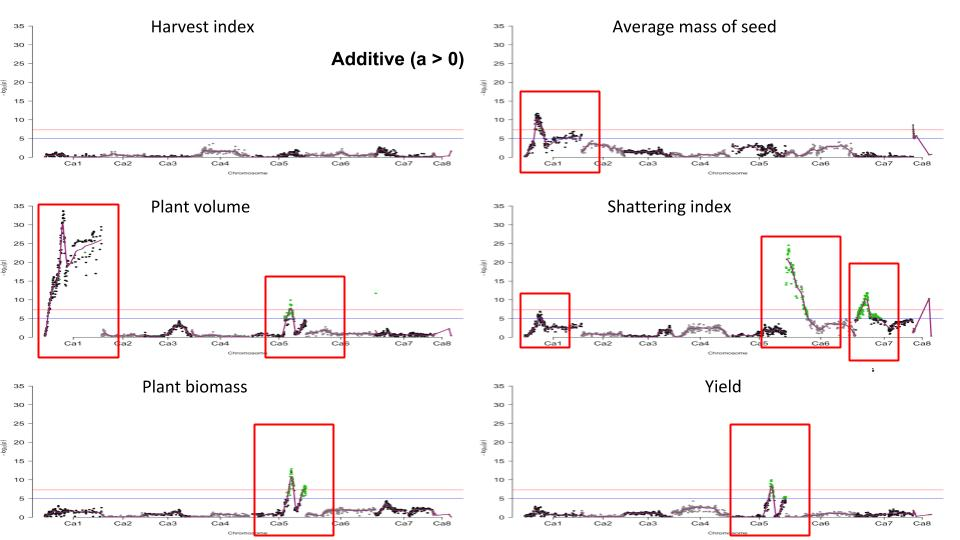
\includegraphics[height=18cm, width=15cm]{tex/chickpea/manhattan-add.jpg}
    \caption{Manhattan plot for p-values of additive effects of all 6 phenotypes. The linear model was set up in such a way that we always interpret the effect of the wild allele in the hybrid. Blue line is for suggestive cut off and red line is for genome wide cut off. In regions that are significant, green dot indicates that the wild allele increases the phenotype.}
    \label{fig:man-add}
\end{figure}

\begin{figure}
    \centering
    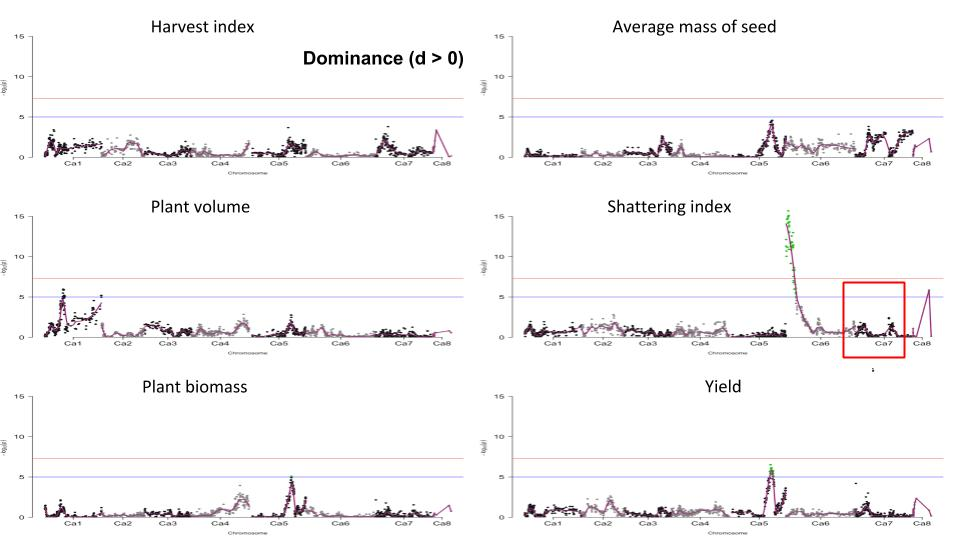
\includegraphics[height=18cm, width=15cm]{tex/chickpea/manhattan-dom.jpg}
    \caption{Manhattan plot for p-values of dominance effects of all 6 phenotypes. The linear model was set up in such a way that we always interpret the effect of the wild allele in the hybrid. Blue line is for suggestive cut off and red line is for genome wide cut off. In regions that are significant, green dot indicates that the wild allele shows dominance and increases the phenotype.}
    \label{fig:man-dom}
\end{figure}

\begin{figure}
    \centering
    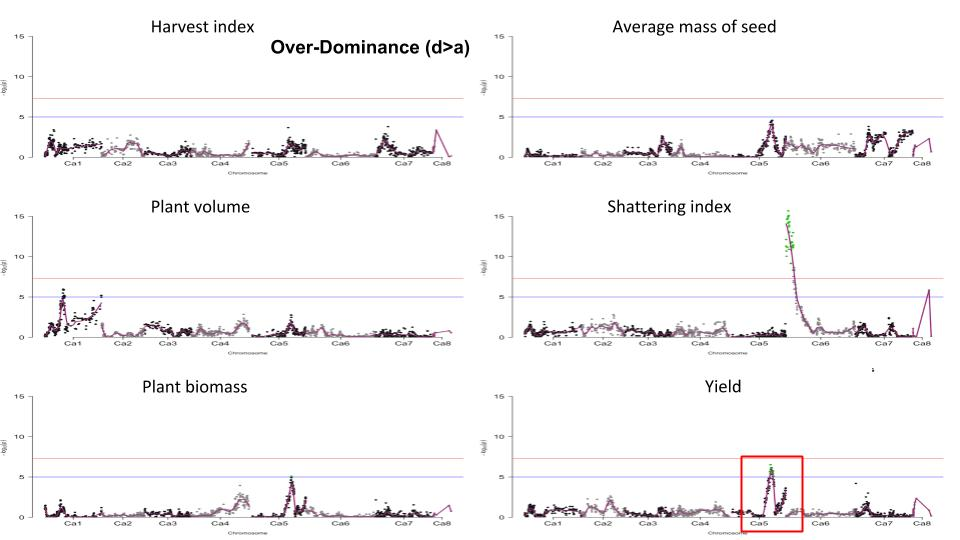
\includegraphics[height=18cm, width=15cm]{tex/chickpea/manhattan-over.jpg}
    \caption{Manhattan plot for p-values of dominance effects of all 6 phenotypes. The linear model was set up in such a way that we always interpret the effect of the wild allele in the hybrid. Blue line is for suggestive cut off and red line is for genome wide cut off. In regions that are significant, green dot indicates that the wild allele shows over-dominance.}
    \label{fig:man-over}
\end{figure}

\section{Conclusion}

Low diversity in domesticated crops is a cause of concern as it reduces resilience of cultivated crops against changes in climatic conditions and ability to resist pathogens. With an increasing population, food security concerns will become more and more acute over the next couple of decades. In such a scenario, it is increasingly imperative to protect existing high yield elite cultivars and produce new breeds that are resilient to changing weather conditions and ecological systems. One possible solution would be to harness diversity back from wild relatives of exiting crop cultivars. 

In order to introgress favourable genomic regions from wilds into elite cultivars, it is necessary to identify the genomic architecture of important agronomic traits. The NAM panels in maize were developed for this explicit purpose and have provided great utility in the breeding program. 

In this chapter, we have introduced the NAM hybrid populations that were grown for chickpea. Since we work with F2 populations, we can also study the dominance architecture of many traits. Here we use GWAS based approaches to study genomic architecture of many traits. We also identify incompatability loci that may point towards viability selection between the two chickpea species. 

% review
\chapter{Post-GWAS: where next? More samples, more SNPs or more biology? \cite{marjoram14}}
\label{cha:research_topic_3}

\section{Introduction}
We live in the era of genome-wide association studies (GWAS), a time in which vast efforts have been made to find single-nucleotide polymorphisms (SNPs) that are associated with phenotypic variation. This has led to the discovery of a large number of associated SNPs— 1617 published GWAS `hits' at $P < 5 \textsc{x} 10^{-8}$ for 249 traits as of the third quarter of 2011, the latest figures available from http:// www.genome.gov. However, there is a growing awareness that the majority of phenotypic variance apparently remains unaccounted for. This has led to a search for this missing heritability (for example, \cite{Manolio2009, Eichler2010} ).

There are at least two possible explanations for missing heritability. First, it may be a consequence of our inability to interrogate all SNPs in a region using so-called SNP-chip array platforms. This has led to a growing enthusiasm for the use of next-generation sequencing technologies with which, in principle at least, all polymorphism in a region can be discovered. However, another possible explanation for missing heritability is that we are not performing the correct analysis of the data we are collecting or we are not estimating heritability in the correct way \cite{Zuk2012}. GWAS typically looks for simple, marginal effects of SNPs on phenotypic variation. However, disease is often complex. As an example, Zuk et al. \cite{Zuk2012} illustrate how simple, nonlinear models can lead to phantom heritability. It is possible (and we believe likely to be) that analyses that move beyond agnostic, marginal tests of association will lead to the amount of missing heritability being significantly reduced. With this in mind, we briefly overview three interconnected pillars of assumptions, which serve as foundations for the marginal GWAS approach: (i) additive genetic variation is abundant, (ii) individual causal polymorphisms have sizable effects and (iii) those polymorphisms segregate at moderate-to-intermediate frequencies. Arguably, a fire has recently begun smoldering under each of these three pillars. We will focus on the brightest flames illuminating the limitations of the traditional GWAS approach. As is frequently the case, these same flames also cast light on possible future directions. Thus, we end on optimistic notes sounded by clues present in recent research.

We begin by discussing each of the three pillars in turn:

\subsection{Pillar 1: Additive genetic variation is abundant}

For decades, programs of stock improvement have relied on the breeders' equation, based on resemblance between relatives \cite{Lynch1998}. These programs have been tremendously successful, resulting in productivity increases of several folds \cite{Falconer1996}. However, the reason why the breeders' equation works remains a subject of debate (and, of course, the plant breeding community has made much progress without it). The problem is that phenotypes arise from principally nonlinear molecular biological processes underlying developmental, signaling and metabolic cascades. Is the additive component of genetic variation, in fact, predominant? Hill et al. \cite{Hill2008} became so alarmed by this issue that they reanalyzed an impressive array of data. They overwhelmingly confirm widespread additivity. They hypothesized that a population genetic process referred to as mutation-selection balance may result in patterns of segregation in casual polymorphisms in which the variation will appear additive even though the pathways through which the phenotypes are affected are highly nonlinear. Indeed, mutation-selection balance can account for most, though hardly all \cite{Houle1998}, of the genetic variation in phenotypes. Under mutation-selection balance most mutations segregating in a population are partially recessive, and they are present at low frequency. Hill et al. \cite{Hill2008} show that under these conditions, most variation will appear additive irrespective of the architecture of the molecular network.

Gjuvsland et al. \cite{Gjuvsland2011} have approached the issue from a different angle, basing their considerations not in population genetics but in network architecture principles. Indeed, population genetics might represent a somewhat shaky foundation upon which to build. If mutations do not contribute to additive variation, natural selection to keep them at low frequency might be ineffective \cite{Charlesworth1996}. If additive variation is removed but non-additive variation accumulates, the outcome might be envisioned as predominantly non-additive variation. Gjuvsland et al. \cite{Gjuvsland2011} show that, in populations with intermediate allele frequencies, randomly generated genotype–phenotype (GP) maps generate proportions of additive heritable variation ($V_a$), among overall variation due to segregating polymorphisms ($V_g$), that are far lower than is empirically observed. They, therefore, argue that the special nature of molecular networks might lead to additivity, even though the networks themselves are nonlinear. As an example of this, they consider the property of `order-preservation', in which the network architecture prevents `order- breaking' \cite{Gjuvsland2011}.

Although both explanations are elegant and intuitive, they in no sense represent a final answer. Indeed, they present particular cases in which $V_a$ would be the main component of variation but they do it by imposing constraints (on the frequency of causal mutations or on network architecture) that do not have to be generally correct. Zuk et al. \cite{Zuk2012} approach the same problem from a different angle. They again start from the common observation that causal polymorphisms detected in GWAS on tens of thousands of individuals appear to account for only a small fraction of heritable variation for a given complex disease. They argue that this conclusion is often drawn because investigators typically, and mistakenly, equate narrow sense heritability, $V_a$, with the estimate of heritability resulting from pedigree studies, $V_g$, which includes effects due to epistasis. This results in a concept they term `phantom heritability'. When compared with $V_g$, much heritability appears to be missing; but when compared (correctly) with $V_a$, much of the missing heritability disappears. Using an example of a particular nonlinear network, they present simulations showing that only a fraction of heritable variation need be truly additive. In such a context, if causal polymorphisms are found as contributing to that truly additive component (rather than highly inflated pedigree-based estimates), the polymorphisms identified would have accounted for most–if not all–of $V_a$. Thus, from their perspective the problem of `missing heritability' should be re-termed as a problem of `inflated $V_a$ estimates'. For a nice overview of issues related to heritability in the GWAS era, see Zaitlen and Kraft (2012)\cite{Zaitlen2012}.

Building on the helpful framework provided by theoretical analyses such as those discussed above, one possible way forward is to analyze genetic variation in the networks directly, observing whether linear models account for a significant fraction of natural variation. We have implemented this approach for sex determination \cite{Tarone2005}, and InR/TOR \cite{Nuzhdin2009} pathways in flies. We proposed \cite{Tarone2012} that small-effect mutations might be well approximated by linearization around steady flow in nonlinear pathways. Whether and to what extent this explanation is generally correct is fertile ground for future research.

\subsection{Pillar 2: Individual causal polymorphisms have sizeable effects}

Inferring causal polymorphisms that account for, but, a tiny fraction of quantitative variation would require an enormous sample size \cite{Long1999}. The sizes of GWAS studies are now reaching multiple thousands of individuals, in part, due to a move toward meta-analysis in recognition of the consequent power benefits (for example, \cite{Lindgren2009,Stahl2010}). However, causal polymorphisms can only be reliably detected if they account for a sizable fraction – on the order of 1\% - of phenotypic variation \cite{Long1999}. Is it reasonable to hope that most polymorphisms have such large effects? The literature on this topic is nearly overwhelming and we are able to cover only a few highlights here. At the beginning of the QTL era, arguments that phenotype would typically be explained by a few loci of major effect were abundant (for example, \cite{Mackay2001}). It was fast realized, however, that the effect sizes are typically overestimated - the so-called Beavis effect (Beavis, 1994). The problem is that the lower the power of an assay, the greater is the resulting overestimation of effect size \cite{Lynch1998}. This is related to the effect known as the `Winner's Curse' in the GWAS field, in which it was also noted that effect sizes for significantly associated loci will typically be overestimated \cite{Kraft2008}.

Is it possible to `back-calculate' the true distribution of the effect size of causal polymorphisms given their estimated effect sizes? Otto and Jones \cite{Otto2000} showed that it is possible to estimate the total number of associated loci from such data, but did not address bias correction. The emerging best practice to avoid the Winner's Curse is to infer the set of causal polymorphisms in one population, whereas estimating their effects in a different, fully independent population \cite{Kruglyak2008}. Although utilizing data from several populations has become a common practice in yeast and human studies, other models do not afford similar replication. In conclusion, the distribution of effect sizes contributing to standing quantitative variation remains unclear.

As an illustration of this in a series of recent manuscripts, Mackay et al. \cite{Mackay2012}, Jordan et al. \cite{Jordan2012} and Weber et al. \cite{Weber2012} identified a relatively small number of candidate polymorphisms that might account for the majority of phenotypic variation. The analytical approaches used rest on the underlying assumption that a few major polymorphisms matter; the conclusions support this conjecture. Alternatively, Ober et al. \cite{Ober2012} reanalyzed some of the same data under a different assumption—the `nearly infinitesimal' model - that assumes numerous polymorphisms, each with rather small effect size. In this paper, they calculate genetic relatedness among genotypes, compare it with phenotypic resemblance and calculate the fraction of phenotypic variation accounted for. The conclusion was that on the order of 8\% of phenotypic variation is explained, consistent with the expectation for the experiment sample size. Overall, genetic polymorphisms appear to have accounted for modest amounts of variation. We stress that the two above analyses, made under diametrically opposed assumptions, resulted in rather divergent conclusions. This is unsurprising as the truth probably represents a mix of larger and smaller effect mutations, and the analyses above pick from opposite tail of this distribution. There has been additional recent progress in this area using models mixing both assumptions in the context of variance component or mixed models \cite{Kang2010, Korte2012}. However, a general picture is yet to emerge.

\subsection{Pillar 3: Individual causal polymorphisms segregate at moderate-to-intermediate frequencies}

The debate over `common mutation - common disease' versus `rare mutations - common disease' models has proven to be the source of a great number of manuscripts, including many recent reviews (for example, \cite{Manolio2009}). We raise this issue only insofar as it relates to the prospect for GWAS. Recall Hill et al. \cite{Hill2008}. If causal polymorphisms are at low frequency, they contribute to additive variation. However, the power to detect such polymorphisms is rather low, potentially requiring prohibitive sample sizes \cite{Zuk2012}. Curiously, as power drops with allele frequency, the resulting expected overestimation of effect size increases \cite{Lynch1998}. Accordingly, less frequent causal polymorphisms will appear to have a stronger effect than is actually the case \cite{Mackay2012}, perhaps biasing the flow of resources from GWAS to the `mutational screen' paradigms that have recently been gaining in popularity \cite{Tennessen2012}.

What proportion of phenotypic variation is, then, due to low-frequency (as compared with intermediate frequency) alleles? Referring back to Mackay et al. \cite{Mackay2012}, Jordan et al. \cite{Jordan2012} and Weber et al. \cite{Weber2012}, low-frequency mutations matter. This is problematic for GWAS if effect sizes are relatively small. However, per the analysis of Ober et al. \cite{Ober2012}, the intermediate frequency alleles matter. This in itself may pose problems for GWAS analyses that focus on detecting additive effects since, as discussed above, although apparent additivity is likely to be for rare variants, it is not a necessary consequence for alleles of intermediate frequency.

To summarize, GWAS will be most successful, if (i) additive genetic variation is abundant, (ii) individual causal polymorphisms have sizable effects and (iii) they segregate at moderate-to-intermediate frequencies. So, is genetic variation mostly additive? In general, we do not know. Do individual causal polymorphisms have sizable effects? Again, in general we do not know. Do they segregate at moderate-to- intermediate frequencies? Once again, we do not really know. Overall, it appears that we are still some way short of certainty in affirming these requirements, at least in the Drosophila model we feature in this chapter.

\section{The way forward: `Post GWAS'}
From the preceding discussion, it is tempting to generalize that the answer ‘we do not know’ is the only ‘true answer’ and the minute one claims that he ‘knows’, he is wrong \cite{Pelevin2001}. This response is obviously unsatisfactory, particularly if it might undermine a paradigm, which is seen as a significant step toward future advances in health and agriculture. Alternatively, might the GWAS paradigm be modified in such a way to result in useful conclusions even if the above pillars are in question?

One feature of the GWAS paradigm is its purely statistical nature. It takes molecular biological knowledge into account only a posteriori. One possible alternative to this is to treat the biological knowledge as prior information, and refocus the analytical approaches accordingly. For example, in Quintana et al. \cite{Quintana2012}, functional information is used to prioritize choice of combinations of SNPs to include in a burden-style association test and thereby gain power.

Another motivation for this alternative perspective is that causal polymorphisms are not directly linked to phenotypes. Instead, a polymorphism has a direct effect only on intermediate processes, such as networks of genes or gene regulatory networks (GRNs). The effect of genotypes is then expressed through their effects on the network themselves. Thus, a polymorphism might affect the level at which a particular gene is expressed, with consequent effects on the products of network(s) in which the gene has a role. Testing association between SNP polymorphism and network parameters means that one can detect the direct association (between SNP and parameter value), rather than the indirect association between SNP and disease phenotype (say). This offers the potential for increased power (regardless of whether or not a SNP is in a gene that is itself in the network).

Drosophila seems to be a prime model for the development of such perspectives. In human and yeast research, GWAS limitations might be overcome, at least partially, by ever increasing the sample sizes. This is not straightforward with flies, where developing and keeping dozens of thousands of natural strains is difficult. As an alternative response, our exquisite knowledge of the molecular processes resulting in the GP map might be capitalized upon to guide fly quantitative geneticists.

Although there might be numerous polymorphisms affecting a network, their effects are stereotypic, that is, they up- or down-regulate genes in the GRN responsible for the GP map. Truly significant advances will be possible once the effects of regulatory polymorphisms are understood as part of the entire GRN. Instead of developing treatments for each of many polymorphisms, a single cure for a specific type of GRN malfunction might be developed–compensating for numerous regulatory polymorphisms at once. Although the accumulation of knowledge necessary for such a paradigm shift might be sufficient in flies, would such an approach ever be practical in human research? We believe the answer is an overwhelming `yes'. We are rapidly entering an era of `personal genomics' wherein `-omics' data (for example, RNA expression, methylation, histone acetylation and protein abundances) will be available for large numbers of cell lines, and ultimately individuals.

Thus, GRNs will rapidly become annotated. Developing GRN-based approaches now, in the first instance with the Drosophila model, will catalyze these advances, providing the conceptual and analytical framework for building GP maps in other species.

\section{Analysis of GRNs: Historical perspective}
As we have discussed, genetic variation does not lead directly to phenotype, but instead alters intermediate molecular pathways that in turn affects the higher-order traits. In order to understand how genetic variation underlies phenotypic variation, we are required to identify the molecular pathways that vary in response to changes in DNA sequence and the environment \cite{Cooper2002, Sieberts2007}. Furthermore, we must consider the interpretation of marginal effects of genes when the genes operate in networks \cite{Cooper2005}. This molecular knowledge has the potential to provide the functional information required not only to identify and validate the susceptibility genes that are directly affected by genetic variation, but also to understand the GRNs in which the susceptibility genes operate, and how changes in these networks lead to disease \cite{Hammer2004, Schadt2008}. Although the above and many other studies considered whole-genome networks, we consider an alternative. Why not start from a small molecularly defined and validated GRN, well described with a precise quantitative model and infer how much variation would such a GRN explain? Although this clearly is an oversimplification, it is a vast improvement over single-gene marginal associations, and it reflects current knowledge accumulated through molecular biology insights.

The most impressive development in this paradigm has occurred in plant breeding, where there is a deep tradition of modeling phenotypes with process-based approaches (the `genotype to phenotype problem'; \cite{Cooper2002, Koduru2008}). Although, traditionally, physiological methods have been used to predict phenotypes for different crop cultivars as they respond to variable environmental inputs \cite{Sinclair1996, Hammer2004}, the most recent trend is to estimate phenotypic outcomes by directly modeling the underlying gene and gene interactions at the expression level \cite{Welch2003, Welch2005a}. In these cases, genes are typically modeled using Boolean logic, linear units, oscillators and so on \cite{Welch2005b, Ravasz2002}. More recently, differential equation-based expression level models of important plant genes have been proposed \cite{Locke2005a, Locke2005b}.

GRN-based models treat a plant as ideally performing, and in a context in which major effect mutations break the GP map, thereby enabling analyses. How should we introduce genetic variation into these models? So far, this integration has relied upon QTL-type inferences \cite{Yin2003, Uptmoor2012}. The goal was to predict environmental effects on plants using different allele combinations of relevant genes, and to better identify the genetic factors that underlie complex environmentally dependent traits \cite{Reymond2003, Tardieu2003, Hammer2004, Quilot2005, Malosetti2006}. It has been shown that inferences from QTL-GRN approaches can be extended to independent genotypes from the same cross \cite{Reymond2003}. QTL-GRN was also helpful for \emph{in-silico} testing of possible allelic QTL or gene combinations \cite{Podlich1998}.

The logical next step is to integrate GWAS with GRN. Would such a combined paradigm hold the promise of accelerating inference? One answer comes from a recent analysis of Wang et al. \cite{Wang2012}, building on Martens et al. \cite{Martens2009}; Gjuvsland et al.\cite{Gjuvsland2010, Gjuvsland2011} and others). Wang et al. \cite{Wang2012} start from a precise GRN model and suppose that it varies among genotypes due to causal polymorphisms. Thereby, a simulated panel of genotypes was used for a GWAS-style analysis. It was also used to back-estimate the variation (among genotypes) for the model parameters given the GRN. The GRN-based approach had far superior power. This is, perhaps, expected as the GRN model used for the data simulation and back-inference was the same. Even with this caveat, this analysis gives hope that GRN-GWAS might account for much more variation than more traditional GWAS approaches. The question remains, however, what are the best statistical practices for such an exercise?

\section{Fitting nonlinear GRNs}
Assume a GWAS panel with the knowledge of genotypes, intermediate molecular phenotypes and whole-organism phenotypes. Assume further that the GRN connecting GP is known–from the analysis of major effect mutations as described above. How would one infer the genotype-specific values of the parameters in the GRN model? This is a cumbersome task \cite{Locke2005b}. Evolutionary algorithms have been successfully applied to simultaneously infer the structure as well as parameters in such networks \cite{Ando2003, Streichert2004}, as have other optimization methods. However, we argue that a more formalized treatment is clearly required and, in particular, such a treatment should effectively capture and report the uncertainty in the inference of the parameters or model structure. We highlight Bayesian methods of network analysis as a powerful alternative tool, with a particular emphasis on a relatively novel method that has come to be known as approximate Bayesian computation (ABC), that remains tractable for extremely complex networks that do not admit closed-form solutions (in which many other analysis paradigms will fail). As such, it allows full description of parameter distributions, and therefore, explicitly capture uncertainty, for even complex models.

As discussed earlier, a Bayesian analysis paradigm proceeds as follows: suppose we have data, $Y$, and wish to infer values of parameters, $\theta$. From a Bayesian perspective, we express this as a posterior distribution, calculated via Bayes Theorem as $f(\theta y|Y) = f(Y|y)\pi(\theta)/f(Y)$. Here $\pi(\theta)$ is the prior distribution. The above assumes the existence of a model, $M$, that describes the underlying processes (in our context a GRN). In other words, the model links the data, $Y$, to the biological parameters $y$. The result of the analysis, the posterior distribution $f(\theta|Y)$, fully characterizes the knowledge regarding the parameters, their uncertainties and the dependencies between them, given the data, in the form of a probability distribution. This allows for a fuller characterization of the underlying models. Credibility intervals for parameter values can then be calculated and goodness-of-fit can be tested for, allowing for model selection (see below). Posterior distributions of relatively low variance indicate situations in which the data leads to a good degree of certainty regarding the parameters values. Conversely, a high variance indicates that little certainty has been obtained.

Sensitivity is captured by examining the posterior distribution for network parameters: parameters to which the network is highly sensitive will have narrow posterior distributions, whereas those that have less influence will have higher posterior variance. This property provides a helpful connection to population genetics–one that may be used to further validate the GRN model. For example, one might hypothesize that the extent to which purifying natural selection will operate can be predicted by a sensitivity analysis of molecular networks. Spontaneous mutations in components of low local sensitivity cause smaller deviations in the network output. Thus, purifying selection will be weak, and functional sequence variation in natural populations will be appreciable. Drift can then cause the appearance of high-frequency mutations, possibly resulting in their fixation. In contrast, mutations causing changes in high-sensitivity components will be eliminated more quickly, they will typically be observed to segregate in natural populations at low frequency, and their fixation between species will not be common. An example of this is seen in Dresch et al. \cite{Dresch2010} and Fakhouri et al. \cite{Fakhouri2010}, where the sensitivity of rho enhancer network was evaluated using different approaches.

The key component of a Bayesian analysis is calculation of the posterior distribution. As discussed in chapter \ref{cha:research_topic_1}, this is often challenging, but a commonly used approach is Metropolis-Hastings Markov chain Monte Carlo methods (MH-MCMC) \cite{Metropolis1953, hastings70}. Although these can be technically challenging to implement, the rapid growth in computational horsepower that we have experienced over the last few decades has resulted in an enormous rise in their popularity. This has led to the production of packages such as \href{http:// www.mrc-bsu.cam.ac.uk/bugs/winbugs/contents.shtml}{WinBUGS} and \href{http://www.openbugs.info/w/}{Open-BUGS} to allow easier implementation of the MCMC method. We illustrate the use of an MCMC analysis of GRN data in Illustrative Example below.

However, despite their flexibility and popularity, traditional Bayesian methods require that one is able to calculate the likelihood function, $f(Y|\theta)$, as, of course, do frequentist approaches. In situations in which this calculation becomes impossible or computationally intractable, an alternative approach must be found. This has lead to the rise of ABC.

\subsection{Approximate Bayesian computation}
ABC methods have been developed over the last decade in response to the recent rapid growth in both the size and complexity of modern data sets and their underlying theoretical models. They allow computationally tractable analyses in contexts in which calculation of the likelihood function becomes impossible. Essentially, they replace calculation of the likelihood with a simulation step, relying upon the fact that rapid simulation of data is often possible in contexts in which calculation has become impossible.

The American statistician John Tukey said `Far better an approximate answer to the right question, which is often vague, than an exact answer to the wrong question, which can always be made precise' \cite{Tukey1962}. ABC methods embrace this spirit by allowing us to use the model we want to use (in this context, a complex, nonlinear GRN), but at the cost of providing an approximate answer. We focus on two ABC methods: those based on accept/reject algorithms and those based on MH-MCMC.

In general, there are two common responses to intractability of the likelihood: (i) simplify the model so that the likelihood function can, once again, be calculated; or (ii) add an approximation step to the analytic method itself. Although approach (i) above is possible, it often leads to a model so divorced from reality that conclusions drawn from it cannot be considered particularly informative. So ABC approaches follow the intuition of both Box and Tukey and adopt approach (ii), constructing approximate answers to the right questions via ABC methods. At this point, we recall a quote attributed to George Box: ‘All models are wrong, but some are useful’.

In the case of the paradigm, we suggest the focus on small networks might be misplaced as they are but a component of larger networks. However, it might be the most helpful perspective, as larger networks are generally not described well enough to quantify, nor are they computationally tractable with the approaches we introduce below. Application to genetic networks is in its infancy, but will allow analysis of pathways that are significantly more detailed, and therefore more realistic, than has been possible using traditional methods. Furthermore, the resulting posterior distributions allow full characterization of the network, thereby capturing, in full, the degree of certainty with which those parameters are estimated, rather than having to rely upon ‘sensitivity analyses’, of the type described in Dresch et al. \cite{Dresch2010}, for example, in the context of transcription networks in \emph{Drosophila}, in which this uncertainty is assessed in a somewhat less comprehensive manner.

\subsection{ABC-accept/reject algorithms (ABC-AR)}
This is perhaps the simplest form of ABC method. Suppose we have a measure of similarity that allows us to determine if two data sets, $D$ and $D'$ are similar (denoted $D \sim D'$). For example, in the example application below, in which the data are a vector of gene expression values, we might use Euclidean distance. Alternatively, a set of summary statistics might be used. The posterior distribution of the associated parameters is estimated using the following iterative procedure:
\begin{enumerate}
    \item Sample parameter values y0 from the prior distribution $\pi(.)$.
    \item Generate a data set $D'$ using the sampled $\theta '$-values (In the present context, this involves simulating output from the network using the $\theta '$-values.).
    \item If $D' \sim D$ then accept $\theta '$. 
    \item Return to 1.
\end{enumerate}

The resulting set of accepted $\theta '$-values form a sample from the posterior distribution $f(\theta | D\sim D')$ \cite{ripley82,rubin84, tavare97}. The details of this form of ABC analysis are dependent on what is meant by $D \sim D'$. If strict equality is used here, so $D'$ and $D$ must be identical, the resulting posterior distribution reflects the distribution of the parameters given the data, $D$. However, in practice, in almost all realistic examples, insisting on an exact match between observation and simulation is impossible (not least because of issues such as measurement error or stochastic noise within the GRN), so a measure of similarity is used. This similarity is often expressed in the form of a set of summary statistics, which must themselves match, or near-match, on observed and simulated data. The details of how all this is done are not always trivial, and a literature is beginning to appear to help investigators with some of these choices \cite{joyce08, nunes10, jung11}.

A variety of other forms of ABC analysis exist, such as ABC versions of MH-MCMC \cite{marjoram03}. Most useful, perhaps, is the Sequential Monte Carlo ABC (SMC-ABC) approach of Del Moral et al. \cite{delmoral06} and Secrier et al. \cite{secrier09}, which is particularly valuable as the number of parameters grows. In this variant of ABC-AR, rather than sampling from the prior one samples from a distribution that changes as the analysis proceeds, and which is designed to more closely approximate the posterior and thereby improve analysis efficiency. The application of SMC-ABC of both Del Morel et al. and Secrier et al. was to simple GRNs. We also note that the package SysBio \cite{Liepe2010} implements both ABC-AR and SMC-ABC, and is designed to integrate with the SBML (Systems Biology Mark-up Language). However, as ABC methods are extremely computationally intensive, for reasons of efficiency purpose-built software is likely to be necessary for any but simple network representations.

\subsection{Model selection in ABC framework}
Another form of analysis that is likely to prove useful in the network context is model selection. Model selection analyses will provide a direct way of linking genotypic variation to the pathway. For example, suppose a SNP, $S$, has an effect on a particular parameter, $\theta p$, of the pathway (for example, because it suppresses gene expression). We might model this by supposing that the individuals in the study population have values of $\theta p$ that depend upon whether the SNP is present or absent. In a Bayesian context, we proceed by supposing that, for each individual, $\theta p$ is drawn from one of two prior distributions, $\pi1$ and $pi2$, and that the choice of distribution is determined by the SNPs.
Clearly, as the number of SNPs available for analysis increases, so will the number of parameter prior distributions. This can be managed by defining the prior distributions for SNPs (say) as a function of meta-information about that SNP, such as functional annotation information.

When full details of a pathway are unknown, model selection can also be used to determine which of two (say) possible representations of a pathway best fit the data. In general, we proceed by including an indicator variable for the specific representation being used at any given moment. For example, in the ABC-AR framework given earlier, we include a variable $I$ to indicate which model is being used in any given iteration. We then define a prior $\pi_M$ over the space of possible models, and define a prior distribution $\pi_{M,\theta}$ for the parameters in each model. We can then adapt the AR algorithm, by replacing step 1 with a new compound step:
\begin{enumerate}
    \item Sample a model $M$ from $\pi_M$; sample parameters for model $M$ from $\pi_{M,\theta}$.
\end{enumerate}
The rest of the algorithm proceeds as before. Now, each accepted iteration will also have a choice of model associated to it. The posterior probability of each model is obtained by integrating out over parameter values at the end of the analysis. So, the posterior probability of model 1, say, is the frequency with which model 1 was used in the accepted iterations. Posterior model probabilities are best interpreted in terms of Bayes Factors (ratios of likelihoods). For example, applications in a network context, including an application to the mitogen-activated protein kinase signalling pathway \cite{Krauss2008,Toni2009a,Toni2009b, Toni2010}.

Although this analysis is straightforward in a general Bayesian context, we note that model selection in an ABC context is more problematic, and remains an active area of research (for example, \cite{Robert2011}).
\section{Illustrative example}
As an example of the analysis of GRNs using the methods discussed in this review, we show results of an analysis of the nonlinear model of the pathway producing expression of Drosophila `gap' genes that pattern the anterior/posterior axis of Drosophila embryos, originally analyzed in Papatsenko and Levine \cite{papatsenko11} and also discussed in chapter \ref{cha:research_topic_1}. This is one of the best-characterized transcriptional networks; an abundance of available functional and genomic information allows us to build quantitative models at multiple levels.

\begin{figure}
    \centering
    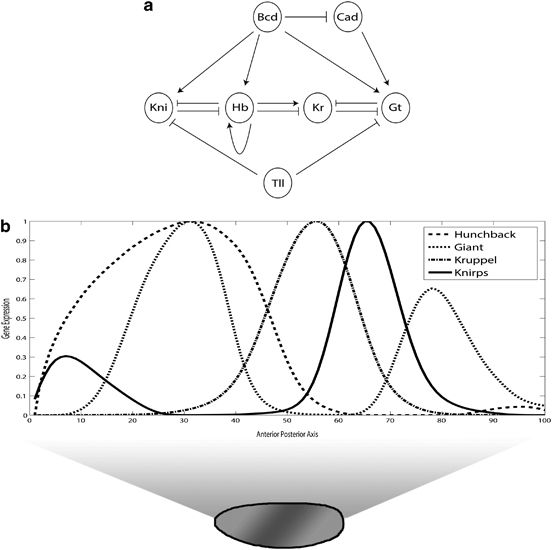
\includegraphics[scale=0.75]{tex/review/hdy201352f1.jpg}
    \caption{(a) Gene regulatory network for Drosophila gap genes, showing relationship between input genes (Bcd, Cad, Hb, Tll) and output genes (Kni,Hb,Kr,Gt). (After figure 1 of Papatsenko and Levine\cite{papatsenko11}). (b) Concentration of Gap genes along the anterior posterior axis of the embryo. Model was fitted to this data. Hb, hunchback; Gt, giant; Kr, Kruppel; Kni, Knirps.}
    \label{fig:review1}
\end{figure}

The Drosophila gap gene network provides early response to maternal gradients in the Dropsophila embryo segmentation pathway. The gap gene’s concentration is set up through cues from maternal genes and mutual repression between the gap genes. Using a modular approach, the gap genes can be divided into network domains, where each domain contains a toggle switch corresponding to a pair of gap genes. The toggle switches resemble the phage lambda bi-stable switch, except the gap genes concentrations are positionally operated through the maternal genes’ gradients with synthesis rates for competing components changing along the anterior–posterior (AP) axis.

Based on this principle, Papatsenko and Levine \cite{papatsenko11} developed a dynamic model for gap gene expression, which exploits elements of fractional site occupancy. The model accounts for diffusion of the gap genes along the AP axis through a system of differential equations and requires five to seven parameters to fit quantitative spatial expression data for gap gene expression gradient. In their paper, Papatsenko and Levine show how the model can account for large effect mutations in the network with a shift in gap gene concentration. The model is illustrated in fig. \ref{fig:review1}.

In this simple example, the network is sufficiently small that it can be solved numerically. Papatsenko and Levine therefore utilized a Metropolis optimization algorithm for fitting their model, where the objective function was based on a measure of correlation between the model and the data. Different fitting ranges were defined for the gap genes along with the length of the embryo.

Of course, such networks include a noise component, both in underlying gene expression and in error of measurement of those expression values. An optimization approach, such as that used in Papatsenko and Levine, will struggle to deal with this, but a fully Bayesian approach remains possible, as we demonstrate using a MCMC analysis. We present results for both a standard MCMC analysis and the ABC variant of MCMC. For a more detailed overview of both methods, see Marjoram and Tavare \cite{Marjoram2006}.

We show the results of such a Bayesian analysis, in terms of the resulting predictive power, in fig. \ref{fig:review2} . In the top row, we show the observed levels of expression (y axis) for each of the four measured genes at each of 100 points sampled along the AP axis of the embryo (x axis). Each gene corresponds to a single column of the figure: Hb, Gt, Kr and Kni (reading left to right). In rows two to four, we show the fits resulting from analyses of that data. In each row, the y axis represents the predicted expression levels. In row two, we show the results obtained by Papatsenko and Levine using a Metropolis optimization algorithm. We note that in that paper they chose to focus on a domain of interest in which the gene expression gradients were greatest, indicated by the region between the two vertical, dashed lines on the plots. In row three, we show results obtained by sampling a single set of parameter values from the posterior distribution resulting from an MCMC analysis of the entire length of the anterior– posterior axis. In row four, we show results obtained by sampling a single set of parameter values from the posterior distribution resulting from an ABC analysis of the entire length of the anterior–posterior axis.
\begin{figure}
    \centering
    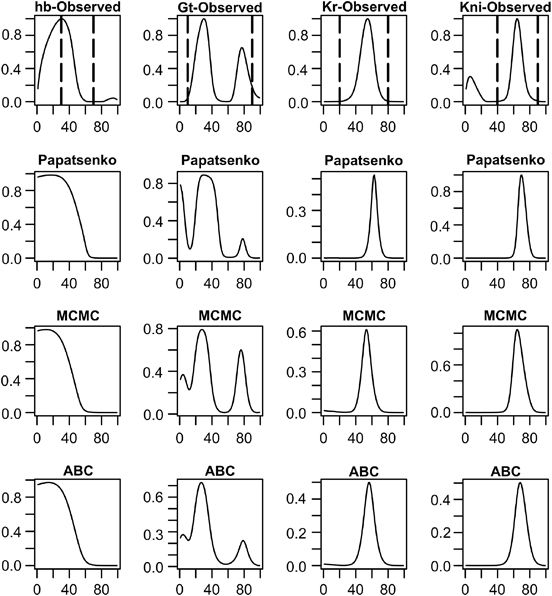
\includegraphics[scale=0.75]{tex/review/hdy201352f2.jpg}
    \caption{Predicted power of analysis of anterior–posterior gap genes for Drosophila. The x axis corresponds to the anterior–posterior axis of the embryo. The y axis indicates the observed (fitted) levels of gene expression in rows 1 (2–4). Top row: observed levels of expression for each of four measured genes: Hb, Gt, Kr and Kni (reading left to right). Row two: fits from Papatsenko and Levine optimization approach. Row three: results sampled from posterior of Bayesian Markov chain Monte Carlo method (MCMC) analysis. Row four: results sampled from posterior of approximate Bayesian computation (ABC) analysis. Vertical lines show the domain of interest of Papatsenko and Levine.}
    \label{fig:review2}
\end{figure}

The figure shows that both the MCMC and ABC analyses fit well. We note in passing that the fit resulting from both the MCMC and ABC analyses over the domain of interest is significantly better than that resulting from the analysis of Papatsenko and Levine, despite the fact that the former analyses fit over the entire length of the embryo. The benefit of the Bayesian approaches is that full posterior distributions are obtained for each of the parameters. As an illustration, we show the posterior distributions resulting from the MCMC analysis in fig. \ref{fig:review3}. We show posterior distributions for four parameters: the cooperativity, C, the synthesis/decay rate, alpha and node-specific binding affinities, K1 and K2. The ABC method typically results in slightly wider posterior distributions for parameters due to the increased tolerance allowed in the analysis. This will likely to be reflected in a reduction in predictive power (seen in fig. \ref{fig:review3}). Thus, it is important to stress that when exact calculation of likelihoods is possible, standard Bayesian approaches, such as MCMC, should be used. However, for more complex (and possibly, therefore, more realistic) networks, an exact MCMC analysis will be impossible, whereas the ABC approach will remain tractable.

\begin{figure}
    \centering
    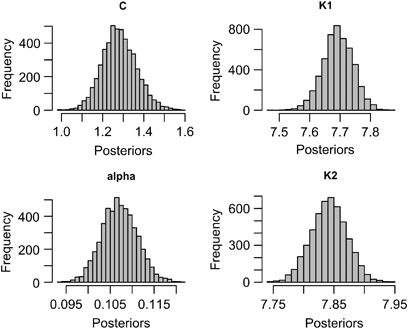
\includegraphics{tex/review/hdy201352f3.jpg}
    \caption{Posterior distributions from Markov chain Monte Carlo method analysis. Shown are distribution for cooperativity, C; synthesis/decay rate, alpha; and node-specific binding affinities, K1 and K2.}
    \label{fig:review3}
\end{figure}

\section{Conclusion}
We are in the middle of a golden age of genetics in which we are discovering unheralded numbers of polymorphisms that are (marginally) associated with phenotypic variance. Although the efforts so far represent a great leap forward, true understanding will only be obtained when we move from association to causation by building an integrated GP map. In doing so, we will not only increase analytic power of discovery, but also move a step closer to impacting human health, as well as animal and plant breeding, in more effective ways. At the same time, we note that stochastic elements that are likely to be present in many networks will mean that complete predictability will never be attained (a statement that is also likely to be true for systems that lack genuine stochasticity, but which are highly complex and will likely therefore never be fully characterized).

In this chapter, we have considered what we have learned so far from the recent flood of GWAS and other data, and in what directions that evidence suggests we should next turn. We do not intend this review as an opinion piece regarding whether GWAS should be labeled as a success or otherwise. We regard this argument to be one of semantics more than content. GWAS has found a large number of polymorphisms associated with phenotype, and will continue to do so. However, it is equally clear that much heritability remains unexplained. Our belief is that now that we have determined what percentage of heritable variation can be explained by polymorphism using marginal statistical analysis (and often using relatively common polymorphism), we face a fork in the road in which one path is labeled `more data', whereas the other is labeled `more biology'. Although both paths are clearly useful, we believe there is much to be gained by considering the latter fork and exploiting the ability of biological knowledge to inform statistical analysis as we attempt to move from association to function, and it is on this perspective that we have focused in this chapter.

Here, our focus has been upon incorporating biological insight via explicit modeling of underlying pathways. However, we also note that there is a growing trend to incorporate biological information into the prior distribution when searching large numbers of SNPs for association with phenotype. For example, one can take information from annotation databases such as \href{http://www. pantherdb.org/}{PANTHER}. This can be viewed as a way of increasing power in the face of increasing multiple comparison penalties.

An advantage of a fully Bayesian analysis of pathways, such as we have proposed here, is that the sensitivity to a given parameter is fully described in the resulting parameter posterior distribution. Given this, we envision the following flow of analysis. Using a Bayesian analysis for each genotype, the parameters important for GRN function are determined. A combination of whole-organism and GRN-specific molecular phenotypes is used. We then infer which GRN perturbation results in which whole-organism phentotype. The relative sensitivities of the phenotypes to perturbations in different GRN nodes and paths are evaluated to select the best targets for disease treatment. When a perturbation of the parameter is detected in a certain genotype, a localized search for the polymorphisms affecting this parameter is made using GWAS-like approaches, focused on specific nodes and/or paths in the GRN. The analyses among genotypes sharing that polymorpshism are then merged to more precisely characterize the effect of the polymorphism on the GRN behavior, much as in a regular GWAS.

This combination of GRN and GWAS approaches will ultimately enable collapsing of the effects of multiple polymorphisms - including those of low frequency—into larger groups of `shared' functional effect. The GRN state, and the effects of groups of functionally similar polymorphisms on that state, could then be compared between individuals experiencing different environments, or between those who are healthy and those who exhibit disease.

Finally, we note that analysis of GRNs such as those we have described here can be extremely computationally intensive, particularly for a method such as ABC. However, ABC approaches also provide several avenues for optimization. In particular, ABC demands repeated simulation from models, and the number of repeats is likely to be very large—the more simulations we perform, the greater the level of agreement between observed and simulated data that can be insisted upon, and therefore the greater (typically) the level of accuracy that can be obtained. It is therefore possible to `parallelize' algorithms and run them over multiple computational nodes, rather than have one node independently simulate data over and over again. N nodes will decrease the analysis time by roughly a factor of N, compared with a single node. This can be achieved on computational ‘clusters’ or, perhaps more cost effectively, by exploiting Graphical Processing Units, which provide extreme increases in computational efficiency when the repeated unit (here the simulation) is relatively straightforward.

In conclusion, we are in the midst of a golden era of genomics, offering the potential to move from association to causation. However, the success of GWAS is likely to be limited by a number of factors. In this chapter, we have discussed some of those factors and offered a possible paradigm for moving forwards form this point in a way that addresses some of those limitations.

% TEs & cancer
\chapter{Suppression of transposable elements in Leukemic stem cells \cite{Colombo2017}}
\label{cha:research_topic_4}

\section{Introduction}
Transposable elements (TEs) were first discovered by Barbara McClintock in the 1940s while studying colouring patterns in maize kernels. Later, it was discovered that large parts of both eukaryotic and prokaryotic genomes consist of transposable elements. Alternatively called `jumping genes' or transposons because of their ability to move (or jump) from one location in the genome to another, TEs are particularly abundant in plant genomes, with 80\% of wheat genome comprising of TEs \cite{brenchly12}. While initially dismissed as `junk' DNA, there is increasing debate on the role of TEs in evolution \cite{chuong16,lisch13}. TEs are also referred to as repeat elements because they are present in multiple copies across the genome. 

TEs are largely categorized by the mechanism of their movement in genomes; those that move by a `copy-and-paste' mechanism using an RNA intermediate (class I retrotransposons), and those that use a `cut-and-paste' mechanism with a DNA intermediate (class II transposons). Due to their ability to make duplicate copies, TEs have been implicated in the increase of genome size. Particularly in angiosperm genomes, that vary over 1000-fold in size, the variation in genome size is strongly correlated with TE content \cite{tenaillon10}. 

Retrotransposons are further classified into long terminal repeat (LTR) and non-LTR elements. Endogenous retroviruses (ERV), which are LTRs, resemble retroviruses in their structure and function. Long interspersed nuclear elements (LINE) such as LINE1 are non-LTRs, and autonomous in their ability to retrotranspose, whereas short interspersed nuclear elements (SINE) such as Alu are non-autonomous, and dependent on LINE for retrotransposition. TEs are highly expressed during embryogenesis and play an active role in it \cite{Gerdes16,Ge17}. TEs have also been suggested to have played a positive role in evolution by increasing the potential for advantageous novel genes \cite{Elbarbary16, Sundaram2014,Thompson2016, Lee2015}.

The genomic regions that contain TEs are highly methylated and are silenced by heterochromatin in the somatic cells \cite{Schulz2006, Groh2017}. TE activation has been reported in aging tissues, including in aging stem cells \cite{Wang2011,Sun2014}. TEs have been reported to be expressed in various types of cancers for the past three decades; however, it remains unknown if they are causal or consequential to the development of cancer. In humans, TEs have been mostly considered detrimental because of their inherent mobile nature. Their expression can lead to insertional mutagenesis, chromosomal rearrangements, and genomic instability, potentially contributing to cancer development \cite{Belancio2015, Kemp2015, Mills2007, Luzhna2015}. 

Recent reports revealed a potential beneficial role of TEs in cancer, wherein ERVs were shown to be potential tumour-specific antigens \cite{Mullins2012}. Hypomethylating agents increase the expression of TEs in cancer cells, inducing `viral mimicry' and causing interferon signalling and cancer cell killing \cite{Chiappinelli2015, Roulois2015}. Bidirectional (sense and anti-sense) transcription of many TEs, including ERVs, yields dsRNA \cite{Lehner2002, Yelin2003}. dsRNA sensors then activate potent interferon response pathways, leading to the activation of inflammatory pathways and cell death \cite{Chiappinelli2015, Roulois2015}. These findings suggested that TE expression in cancer cells could play a role in immune-mediated clearance of cancer cells.

Acute myeloid leukaemia (AML), the most common form of acute leukaemia in adults, is characterized by high rates of initial remission with chemotherapy (60 - 70\%), but is also associated with high relapse rates. Nearly two decades ago, it was shown that only a small fraction of AML cells (termed leukemic stem cells or LSCs) were capable of re-initiating the tumour when transplanted into immunodeficient animals \cite{Bonnet1997}. LSCs in AML can be identified based on the expression of cell surface proteins ($CD34^+CD38^{neg}CD99^+TIM3^+$) \cite{Corces2016}. Although the exact role of LSCs in the pathogenesis and relapse of AML is still debated, their presence is associated with resistance to therapy, relapse, and poor prognosis \cite{Reinisch2015}. Thus, targeting LSCs in AML is a major focus of oncologic research, however the lack of understanding of pathways dysregulated in LSCs has hampered progress. We speculated that the resilience of LSCs was mediated by its ability to escape immune mediated clearance. To investigate this, we studied the expression of TEs and its accompanying immune pathways in AML cell fractions.

\section{Materials and Methods}

\subsection{ATACseq data analysis}
ATACseq fastq reads were analyzed from Corces et al \cite{Corces2016}. Patient trios were selected which had ATACseq data from pHSC, LSC and Blast samples. ATACseq reads were aligned against the hg19 reference genome using the \href{https://arxiv.org/abs/1303.3997}{bwa mem algorithm}. Following the alignment, QC was performed for the samples. Only reads aligned to autosomes and sex chromosomes were considered. Mitochondrial reads were discarded.

All samples showed enrichment for transcription start sites (TSSs) sites. Enrichment was computed by comparing total reads falling into a window of 2kb just upstream of promoters to reads in a 5kb window distant from the TSS. An important visualisation tool for ATACseq data is the distribution of fragment sizes. A typical fragment size distribution showed a characteristic wiggle indicating large fraction of short nucleosome-free fragments and a lower fraction of fragments from regions protected by nucleosomes \cite{Buenrostro2013, buenrostro2015}. We used the getPESizes function from the csaw \cite{Lun2016} library to interrogate the distribution of fragment sizes.

Our goal in this analysis was to compare changes in chromosome accessibility across cell-types. This falls within the framework of differential accessibility testing. Here we favored adoption of a window-based method \cite{Lun2014} for detecting differentially accessible regions. Such approaches have previously been implemented for ChIPseq data, notably in the package csaw \cite{Lun2016}.

Reads were counted along the chromosomes in sliding windows of size 200bps. Windows with less than 10 reads were discarded. Further filtering was done by first computing a global background of reads distribution by counting reads in contiguous window size of 1000bps. Composition bias across libraries was alleviated by normalising the libraries using the trimmed mean of M-values (TMM) method \cite{Robinson2010}. Read counts in contiguous windows of 1000bps were again considered for this purpose.

Post normalisation and filtering, the libraries were used for calling differentially accessible windows across cell-types. A paired design ($Y \sim patient + cell type$) was employed to perform a negative binomial regression using functions from the edgeR \cite{Lun2016}. Differentially accessible windows for LSC versus Blast samples and LSC versus pHSC samples were tested for. Post accessibility testing, neighbouring windows were combined to define a region and significance level of the region computed from the p-values of the window-level tests. Multiple testing correction was then done at the region-level using a False Discovery Rate (FDR) cut-off of 0.01. For interpretability of the regions, the number of log-fold change increase (logFC UP) and log-fold change decrease (logFC DOWN) windows it contained were also computed. In addition, the p-value of the best window and the direction of change were also reported. Finally, all regions were annotated to report their distance from neighbouring genes.

\section{Results}

\subsection{LSCs show low expression of TEs.}
Corces et al. \cite{Corces2016} had recently used fluorescent activated cell sorting to isolate leukemic cells from patients with AML. They separated the cells of three distinct stages of AML evolution, pre-leukemic haematopoietic stem cells (pHSCs; $CD34^+CD38^{neg}CD99^{neg}TIM3^{neg}$), leukemic stem cell (LSCs; $CD34^+CD38^{neg}CD99^+TIM3^+$), and leukemic blasts (Blasts; $CD99^+TIM3^+CD45^{mid}SSC^{high}$), characterized their transcriptome, and analysed their coding gene expression patterns \cite{Corces2016}. To investigate the regulation of TEs in the development of AML, we examined the transcriptomes in these stages by measuring the changes in TE expression. When LSCs were compared to pHSCs and Blasts, we identified a significant downregulation of TEs in LSCs (Fig. \ref{fig:tes1} a,b). Among the different classes of TEs, SINE was the most suppressed in LSCs, followed by LTR retrotransposons (Fig. \ref{fig:tes1} a). The most dysregulated TE types in LSCs were Alu, ERV1, ERVL, ERVK, and LTR retrotransposons, all of which showed significant suppression.

We further analysed the dysregulation of TEs in individual AML samples, while tracking the stages of AML. We found that specific TE types were dysregulated, with LSCs showing significant suppression of Alu, ERV3. ERVK, ERVL, and LTR retrotransposons (Fig. \ref{fig:tes1} c). We did not observe significant suppression of LINE1 in LSCs. These results suggested that TEs were dysregulated during AML development, with LSCs showing significant suppression of specific TE types.

\begin{figure}[h!]
\centering
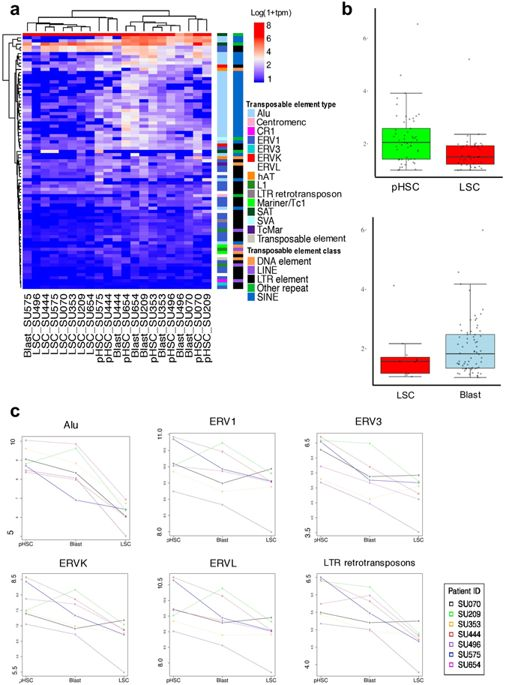
\includegraphics[scale=0.8]{tex/tes/41598_2017_7356_Fig1_HTML.jpg}
\caption{Analysis of differential expression of transposable elements in pre-leukemic stem cells (pHSC), leukemic stem cells (LSC), and Blasts (a) X-axis; Patient identifier.  The expression levels in log10 using the metric transcripts per million (TPM).  The `Transposable Element (TE) Type' classifies individual repeat transcripts into one of 68 unique canonical categories of TEs. Each TE type is contained in one TE Class. (b) Quantiles of the absolute log-fold change of the differentially expressed (DE) TE transcripts in pHSC-LSC, and Blast-LSC samples. Y-axis: absolute log-fold change of each individual DE TE transcript from Fig. \ref{fig:tes1}A. (c) Y-axis: log10 of TPM expression level for each of the 7 paired samples across each clonal point.  The individual patients are denoted with unique colours.}
\label{fig:tes1}
\end{figure}


\subsection{LSCs show suppression of interferon pathways.}
LSCs are known to be resistant to treatment and serve as potential sources of relapse for AML, although the mechanisms behind this resilience are not fully understood \cite{Reinisch2015}. Expression of TEs is known to activate a viral recognition pathway, which causes interferon signalling and immune-mediated cell clearance \cite{Chiappinelli2015, Roulois2015}. Because LSCs showed suppressed TE expression, we investigated whether this TE suppression was associated with the suppression of interferon pathways in LSCs, which could enable its escape from immune-mediated clearance. LSCs showed significantly higher suppression of several Gene Ontology Consortium (GO)-interferon signalling pathways than Blasts (Fig. \ref{fig:tes2}a). When immune-related pathways (with a set of 335 genes, generated by combining 17 canonical immune pathways in MSigDB) and inflammatory pathways (with a set of 649 genes combining acute inflammatory response and inflammatory response in MSigDB and GO) in LSCs and Blasts were compared, LSCs showed significant suppression of the immune-related pathways (Fig. \ref{fig:tes2}b).

However, comparison between LSCs (which showed lower expression of TEs than pHSCs) and pHSCs showed no significant differences in interferon, immune, or inflammatory pathways. This appeared to contradict the model of TE-induced activation of immune pathways. We therefore investigated alternate pathways that could suppress in immune pathways in pHSCs. Interestingly, we found that all pHSCs exhibited very high expression of EVI-1 (pHSCs vs. LSCs, 4.6-fold, $p < 0.0001$; pHSCs vs. Blasts, 3.4-fold, $p < 0.0001$), which is known to suppress immune pathways by downregulating NFκB (a pathway known to be activated by viral RNA) \cite{Xu2012}. Consistent with this finding, we also observed that NF$\kappa$B pathways were more suppressed in pHSCs than Blasts (Blasts and pHSCs showed similar expression of TEs). These findings suggested that both LSCs and pHSCs showed suppression of NF$\kappa$B and immune-related pathways, compared to Blasts. LSCs showed suppressed TE expression and pHSCs showed high expression of EVI-1.

\begin{figure}[h!]
\centering
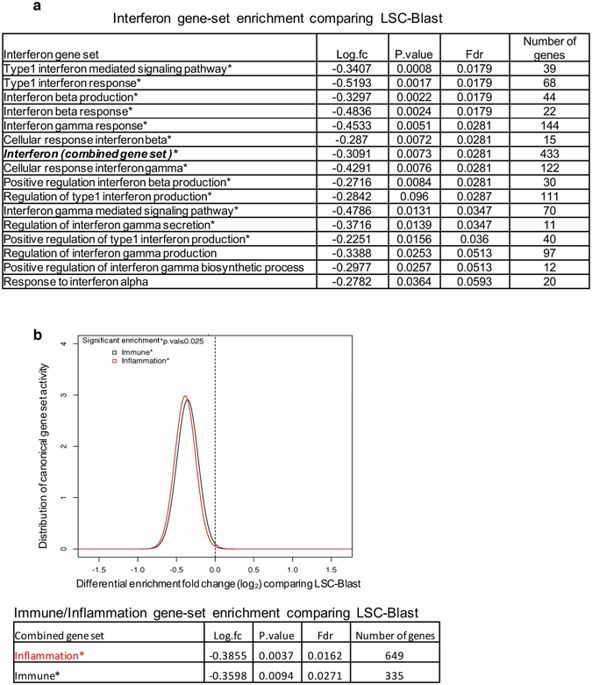
\includegraphics[height = 15cm, width = 15cm]{tex/tes/41598_2017_7356_Fig2_HTML.jpg}
\caption{Analysis of gene set enrichment for interferon, inflammation, and immune response genes (a) Interferon-related gene sets from GO MSigDB, comparing LSCs and Blasts in AML. (b). Gene set enrichment analysis of combined inflammation and immune gene sets, comparing LSCs and Blasts.  The Bonferroni multiple testing correction significance threshold is denoted as `p.val'. * indicates p \textless 0.025.}
\label{fig:tes2}
\end{figure}

\subsection{Coding gene networks are co-regulated with TEs}
Although TE expression is known to activate immune pathways, the types of TEs that participate in this mechanism are currently unknown. In order to understand the relationship between coding gene expression and the expression of specific TE subtypes, we first performed an unsupervised clustering of the AML samples based on coding gene expression, and found that LSCs formed a well-grouped cluster (Fig. \ref{fig:tes3}). We then analysed the corresponding expression of various TE types and observed a significant suppression in the expression of specific TE types such as Alu, ERV3, ERVK, and LTR ret- rotransposons in LSCs, compared to pHSCs and Blasts (Fig. \ref{fig:tes3}). This suggested that coding gene expression was distinct in samples with low expression of specific types of TEs (LSCs).

Next, in order to investigate which coding gene networks were correlated with specific TE types, we created a genomic association table using the transcriptome from Blasts and LSCs, as shown in Fig. \ref{fig:tes4}. The coding genes were first clustered based on their co-expression to form specific modules. Each module contained unique set of genes that were likely co-regulated and had functional similarities. %For example, module 26 contains many RNA helicase genes (Supplement Fig. 5). 
We correlated these modules to the expression of specific TE types and found that some modules were positively or negatively correlated with the expression of specific TE types. We performed a pathway analysis using the genes in each module for testing the interferon, immune and inflammatory activity, comparing Blasts to LSCs. We identified modules that showed activation (modules 3, 5, 13, 14, 17 and 41) and suppression (22, 24, 26, 29, 30, 39 and 46) of interferon/immune/inflammation gene pathways in Blasts, compared to LSCs (Fig. \ref{fig:tes4}). We then correlated this with the expression of different TE types. As shown in the Fig. \ref{fig:tes4}, the modules that had shown activation of interferon/immune/inflammation genes were positively associated with the expression of specific TE types (Alu, ERVL, ERVK, and LTR retrotransposons) and negatively associated with the expression of ERV1, SAT, and L1. The modules that had shown suppression of the genes in interferon/immune/inflammation were positively associated with the expression of ERV1 and negatively associated with Alu, ERV3, ERVL, and LTR retrotransposons. Chi-square test confirmed a global association between the correlation of positive/negative coding gene module with TE types and the positive/negative enrichment activity of the interferon/immune/inflammation pathways, respectively (p \textless 0.005). This suggested that specific types of TE were significantly linked to interferon/immune/inflammatory pathway activation.

\begin{figure}
    %\centering
    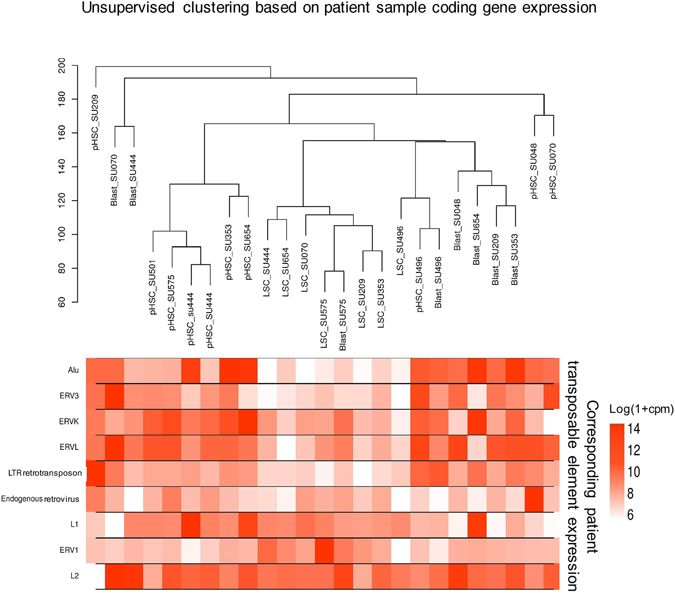
\includegraphics[height = 15cm, width = 15cm]{tex/tes/41598_2017_7356_Fig3_HTML.jpg}
    \caption{Unsupervised hierarchical clustering of coding gene expression in patient samples and the expression levels of the corresponding transposable elements (a)  The image on top depicts the hierarchical clustering of each group (pHSC, LSC, and Blast) based on the average Euclidean distance for the coding gene expression in the patient samples. Below each sample, the expression of the corresponding TE Types (Alu, ERV3, ERVK, ERVL, LTR Retrotransposon, Endogenuous Retroviruses, L1, ERV1, and L2) is shown.  The TE expression is expressed in units of normalized counts per million (CPM) of log10 (1 + CPM).
}
    \label{fig:tes3}
\end{figure}

\begin{figure}
    \centering
    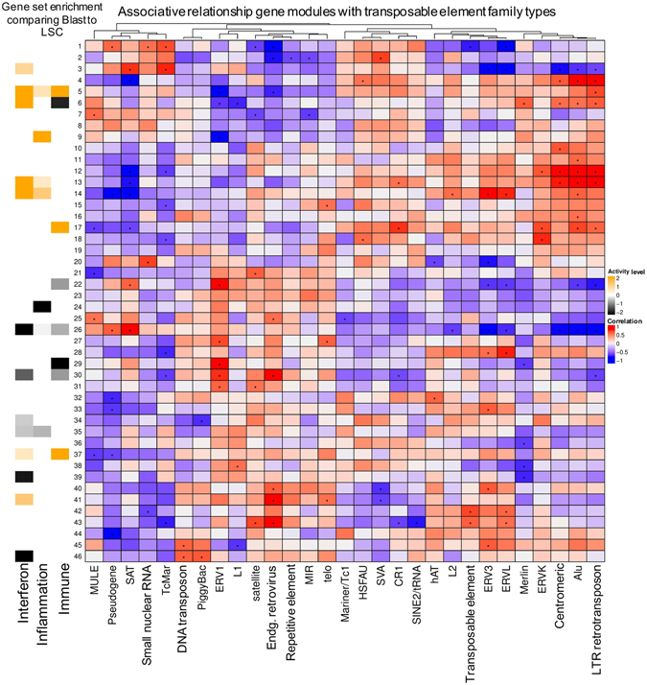
\includegraphics[height = 15cm, width = 15cm]{tex/tes/41598_2017_7356_Fig4_HTML.jpg}
    \caption{Identifying significant associations between the expression of coding gene network and the transposable element types in AML.  The numbers on the Y-axis denote the gene `modules' constructed by identifying gene networks based on co-expression patterns.  The X-axis denotes canonical TE types used for correlating them. The centre  figure of squares represents the correlation matrix for the normalized gene `module' expression and the TE type. * indicates significant associations (p.value \textless 0.05). Each gene `module' was tested for activation of canonical immune and inflammation gene sets in Blasts and compared with LSCs.  The significant (p.value \textless 0.05) pathway activity level for each module is plotted on the left  of Y-axis (yellow indicates significantly higher activation in Blast, and black indicates significantly higher activity in LSCs).}
    \label{fig:tes4}
\end{figure}


\subsection{Pathways that potentially mediate suppression of TEs in LSCs}
The mechanisms behind the regulation of TEs have not been thoroughly investigated. Similar to coding genes, TEs can be regulated both transcrip- tionally and post-transcriptionally. Epigenetic modifications secondary to alterations in ATRX, P53, and SIRT1 and methylation of DNA, have been shown to regulate the expression of TEs \cite{Leonova2013,Elsasser2015,Meter2014}. We investigated whether TEs were suppressed in LSCs through epigenetic mechanisms by analysing its chromatin accessibility using the data from assay for transposase accessible chromatin with high-throughput sequencing (ATAC-seq) for pHSCs, LSCs, and Blasts from Corces et al. \cite{Corces2016}. ATAC-seq has been used for genome-wide mapping of chromatin accessibility. It uses Tn5 transposase to insert sequencing adapters into accessible regions of the chromatin and then uses the sequence reads mapped to the genome to infer accessible regions. Principle component analysis showed that pHSCs were clustered separately from LSCs and Blasts (Fig. 6a). Contrary to our expectations, LSCs, despite having low expression of TEs, had more nucleosome-free regions than pHSCs (Fig. \ref{fig:tes6}b). We analysed the differential accessibility by comparing the accessibility of LSCs to pHSCs, and found 18,099 regions that were significantly more accessible and 441 regions that were significantly less accessible in LSCs compared to pHSCs (Fig. \ref{fig:tes6}b). Comparison of LSCs to Blasts showed no significant differences in the accessible regions. These findings suggested that the suppression of TEs in LSCs was likely not due to increased heterochromatin.

\begin{figure}
    \centering
    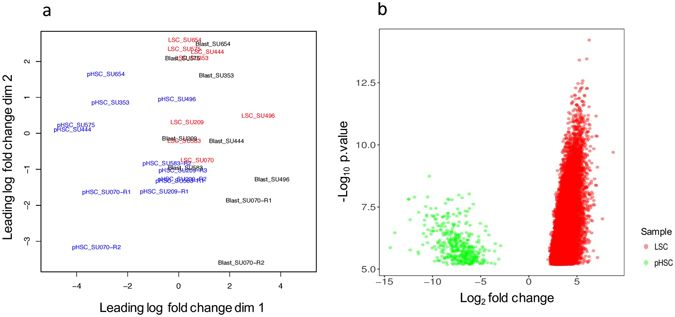
\includegraphics[height = 15cm, width = 15cm]{tex/tes/41598_2017_7356_Fig6_HTML.jpg}
    \caption{Chromatin accessibility in pHSCs, LSCs, and Blasts (a) Multi-dimensional scaling plot with two dimensions showing similarity between di erent ATACseq samples: pHSC (blue), LSC (red), and Blast (black). (b) Depicts the differential accessibility using ATACseq sampling data comparing LSCs to pHSC. X-axis is log2 fold change of differentially accessible regions; Y-axis is –log10 of the p.values reported from comparison.  The minimum p.value considered was $5.593e-03$.}
    \label{fig:tes6}
\end{figure}

Because LSCs showed suppressed TE expression despite having more accessible chromatin, we investigated other pathways that could regulate TE expression. A major mechanism for regulating TEs involves their post-transcriptional degradation \cite{Goodier2012,Goodier2013}. We analysed genes known to suppress TEs post-transcriptionally, as described by Goodier et al.\cite{Goodier2016}28, and compared them in LSCs and Blasts. LSCs showed significant upregulation of ATG5 and KIAA0430 (Fig. \ref{fig:tes7}a). Similar to the piRNA system in males, KIAA0430 or meiosis arrest female protein 1 is known to play a key role in repressing TEs during oogenesis \cite{Su2012}. However, its role in regulating TEs in somatic cells has not been reported. Autophagy-related 5 (ATG5), which was significantly upregulated in LSCs, mediated autophagy by enabling the formation of autophagy vesicles. Autophagy is a process by which various intracellular components are transported to the lysosomes and degraded. A recent study showed that autophagy mediates the degradation of TE post-transcriptionally \cite{Guo2014}. Interestingly, LAMP2 was also upregulated in LSCs (Fig. \ref{fig:tes7}b). Recently, it was shown that LAMP2C, a splice isoform of LAMP2, mediated the degradation of RNA via autophagy (RNAutophagy) \cite{Fujiwara2013, Fujiwara2015, Hase2015}. HSP90AA1 (heat shock protein 90 kDa $\alpha$ [cytosolic], class A member 1) is a pathogen receptor that activates autophagy and thus controls the viral infection \cite{Hu2015}. This protein was also seen upregulated in LSCs (Fig. \ref{fig:tes7}a and b).

\begin{figure}
    \centering
    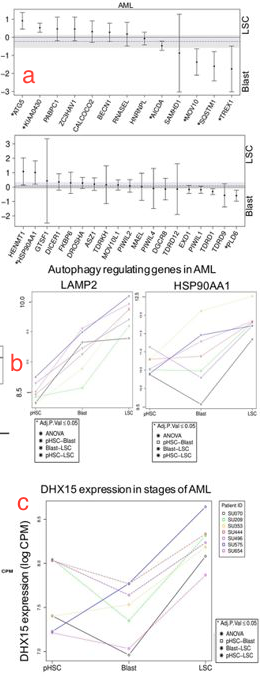
\includegraphics[scale=0.8]{tex/tes/fig7-aml.png}
    \caption{Expression of genes that modulate transposable elements post-transcriptionally (a) Genes that regulate TE post-transcriptionally. Positive fold-change (Y-axis; y \textgreater 0) indicates higher expression in LSCs. Negative fold-change (y \textless 0) indicates higher expression in Blasts. Significant genes are denoted with * p.value \textless 0.05. (b) Autophagy-regulating genes in AML. Expression of LAMP2 and HSP90AA1 pairwise comparison of AML stages. Paired patient measurements are shown with matching colours. Adjusted significance values denoted * p.value \textless 0.05 (c) Expression of RNA helicase genes, DExH genes. Expression of DHX15 in different stages of AML, where paired patient measurements are shown with matching colours. Adjusted significance values denoted * p.value \textless 0.05.}
    \label{fig:tes7}
\end{figure}

RNA helicases are known to bind to and degrade TE post-transcriptionally \cite{Goodier2016,Goodier2012,Bryk2001, Ott2014,Taylor2013, Wu-Scharf2000}. In particular, DHX15 was significantly upregulated in LSCs, compared to Blast (Fig. \ref{fig:tes7}c). These results indicated the possibility that several post-transcriptional mechanisms operated for mediating the suppression of TEs in AML.

\section{Discussion}
Our study is the first to comprehensively evaluate the expression of TEs and its association with coding genes in cancer. We demonstrated that the expression of TEs was dysregulated during the development of AML, with LSCs showing significant suppression. It has been shown that the suppression of the viral recognition pathway conferred resistance to chemotherapy; mutations in MAVS and RIG-1, genes in the viral recognition pathway, have been reported in cancer \cite{Ranoa2016}. We speculated that the expression of TEs could be a potential mechanism for immune-mediated elimination of cancer cells.

Hypomethylating agents have been found to be useful for treating AML, and recent studies have reported that the activation of TEs with the subsequent immune activation was important for their efficacy against cancers \cite{Chiappinelli2015, Roulois2015}. Here, we demonstrated that these mechanisms likely operated naturally during cancer development and progression to enable immune-mediated control of AML. Despite the efficacy of hypomethylating agents against AML, only a minority (~20\%) of patients responded to this therapy \cite{Yun2016}. Among patients who did respond, most eventually developed resistance to therapy with hypomethylating agents. Understanding the regulation of TEs would help us explore predictive factors for hypomethylating treatment and develop novel strategies to prevent relapse in patients treated with hypomethylating agents.

The role of LSCs in the pathogenesis of AML remains controversial. Our results showed that LSCs clearly suppressed the expression of TEs along with distinct coding gene expression. They also showed more suppression of inflammatory pathways, including the NF$\kappa$B pathway. Since Blasts are short lived, they probably did not evolve mechanisms to escape immune-mediated attacks. We speculate that LSCs are a subset of Blasts with the ability to evade immune recognition.

pHSCs, despite having similar expression levels of TEs as Blasts, also showed suppression of inflammatory pathways that prevent the activation of immune signalling. EVI-1, which is known to suppress NF$\kappa$B, was uniquely over-expressed in pHSCs, suggesting that there exists distinct genes which suppress the inflammatory pathways in pHSCs. pHSCs carry mutations in genes regulating the epigenetic machinery and have been clearly demonstrated to precede the development of AML \cite{Jan2012}. pHSCs are resistant to chemotherapy and likely function as reservoirs for relapse of leukaemia \cite{Corces-Zimmerman2014a, Corces-Zimmerman2014b}. High expression of TEs in pHSCs makes them vulnerable to clearance through the viral-recognition pathway; however, this event likely never occurs because of EVI1-mediated suppression of NF$\kappa$B, which is downstream to the viral-recognition pathway. High expression of EVI-1 has been shown to be an indicator of poor risk in AML \cite{Haas2008}. Our analysis is the first to highlight that EVI-1 was significantly expressed at high levels in pHSCs. Targeting EVI-1 in pHSCs could help prevent clonal evolution in AML. For example, miR-133 is known to target EVI-147. It would be important to explore its role in clonal haematopoiesis in the elderly, a condition characterized by expansion of haematopoietic stem cells with mutations in pHSCs.

Our analysis that correlated the expression of coding gene networks to the expression of TE types revealed an association between inflammatory pathways to SINE and LTR families and an anti-association with LINE1. Among the types of TEs, LINE1 is known to have the highest activity of retrotranspositioning and thus has the most potential to cause genomic instability. Hence, LSCs might have co-opted to evolve by suppressing the inflammation-inducing TE classes, while retaining the expression of LINE1, which could potentiate genomic instability and hence clonal evolution.

%We found high expression of several DExH RNA helicases in high-risk MDS. Recent study by Aktas et al. showed that suppression of DHX9 lead to increased levels of Alu48. DHX9 was one of the RNA helicases upregulated in LSCs and high-risk MDS in our study. Targeting DHX9 hence could lead to activation of cancer immunogenicity. Importantly, DHX9 is currently being explored as a target for cancer therapy49–53. RNA helicases bind to single as well as double stranded RNA, and regulate gene splicing. Aberrant splicing events have been reported in patients with MDS, but it is not known whether these splicing factors also regulate TEs. Exploring this function of RNA helicases would enable us to develop drugs targeting them to activate TEs in AML and MDS. In addition to RNA helicases, the role of autophagy in protecting cancer cells from immune attacks via suppressing TE needs to be explored. Drugs targeting autophagy, RNA autophagy (mediated by LAMP2C) in particular, could be promis- ing therapeutic agents against AML and MDS.

Immuno-oncology is emerging as one of the cornerstones of treatment of various cancers. Interferons have long been used in the treatment of cancers, leading to sustained remissions \cite{Talpaz2013, Ortiz2017, Hasselbalch2011}. However, it has been associated with significant systemic toxicities. Activating suppressed TEs, which are known to activate interferons, in cancer cells could potentially accomplish this in a targeted manner.

Our study is the first to show dysregulation of TE in LSCs, revealing its importance in the pathogenesis of AML. Studying direct mechanisms of the regulation of cancer immunosurveillance by TEs in AML could lead to therapies improving long-term survival by manipulating the expression of TEs in leukemic cells.


\chapter{Conclusion}
\label{cha:conclusion}

In this dissertation, we have presented and elaborated on the  Bayesian framework and its utility in tackling various problems in biology. Starting with an application of Bayesian model selection, we elaborate and show an analysis of association analysis. Thereafter, we critically examine the limitations of association mapping analysis particularly as they pertain to the approach to GWAS. We offer perspectives on moving forward and describe how Bayesian approaches can be used to integrate quantitative genetics and systems biology approaches. Finally, we take a side-step and discuss an important analysis in cancer pertaining to expression of transposable elements. 



\begin{singlespace}
  % Bibliography
  \references{plain}{references}

  \appendix
  % Appendices
  \chapter{Appendix}
\label{appendix}
\section{Population genomic analysis uncovers African and European admixture in \emph{Drosophila melanogaster} populations from the south-eastern United States and Caribbean Islands \cite{kao15}}

Drosophila melanogaster is postulated to have colonized North America in the past several 100 years in two waves. Flies from Europe colonized the east coast United States while flies from Africa inhabited the Caribbean, which if true, make the south- east US and Caribbean Islands a secondary contact zone for African and European D. melanogaster. This scenario has been proposed based on phenotypes and limited genetic data. In our study, we have sequenced individual whole genomes of flies from populations in the south-east US and Caribbean Islands and examined these popula- tions in conjunction with population sequences from the west coast US, Africa, and Europe. We find that west coast US populations are closely related to the European population, likely reflecting a rapid westward expansion upon first settlements into North America. We also find genomic evidence of African and European admixture in south-east US and Caribbean populations, with a clinal pattern of decreasing propor- tions of African ancestry with higher latitude. Our genomic analysis of D. melanogas- ter populations from the south-east US and Caribbean Islands provides more evidence for the Caribbean Islands as the source of previously reported novel African alleles found in other east coast US populations. We also find the border between the south- east US and the Caribbean island to be the admixture hot zone where distinctly Afri- can-like Caribbean flies become genomically more similar to European-like south-east US flies. Our findings have important implications for previous studies examining the generation of east coast US clines via selection.

\newpage

\section{Translating natural genetic variation to gene expression in a computational model of the \emph{Drosophila} gap gene regulatory network \cite{gursky2017}}
Annotating the genotype-phenotype relationship, and developing a proper quantitative description of the relationship, requires understanding the impact of natural genomic varia- tion on gene expression. We apply a sequence-level model of gap gene expression in the early development of Drosophila to analyze single nucleotide polymorphisms (SNPs) in a panel of natural sequenced D. melanogaster lines. Using a thermodynamic modeling frame- work, we provide both analytical and computational descriptions of how single-nucleotide variants affect gene expression. The analysis reveals that the sequence variants increase (decrease) gene expression if located within binding sites of repressors (activators). We show that the sign of SNP influence (activation or repression) may change in time and space and elucidate the origin of this change in specific examples. The thermodynamic modeling approach predicts non-local and non-linear effects arising from SNPs, and combi- nations of SNPs, in individual fly genotypes. Simulation of individual fly genotypes using our model reveals that this non-linearity reduces to almost additive inputs from multiple SNPs. Further, we see signatures of the action of purifying selection in the gap gene regulatory regions. To infer the specific targets of purifying selection, we analyze the patterns of poly- morphism in the data at two phenotypic levels: the strengths of binding and expression. We find that combinations of SNPs show evidence of being under selective pressure, while indi- vidual SNPs do not. The model predicts that SNPs appear to accumulate in the genotypes of the natural population in a way biased towards small increases in activating action on the expression pattern. Taken together, these results provide a systems-level view of how genetic variation translates to the level of gene regulatory networks via combinatorial SNP effects.


\newpage

\section{Genetic Diversity, Population Structure, and Genetic Correlation with Climatic Variation in Chickpea (\emph{Cicer arietinum}) Landraces from Pakistan \cite{Sani2018}}

Chickpea (Cicer arietinum L.) production in arid regions, such as those predominant in Pakistan, faces immense challenges of drought and heat stress. Addressing these challenges is made more difficult by the lack of genetic and phenotypic characterization of available cultivated varieties and breeding materials. Genotyping-by-sequencing offers a rapid and cost- effective means to identify genome-wide nucleotide variation in crop germplasm. When combined with extended crop phenotypes deduced from climatic variation at sites of collection, the data can predict which portions of genetic variation might have roles in climate resilience. Here we use 8113 single nucleotide polymorphism markers to determine genetic variation and compare population structure within a previously uncharacterized collection of 77 landraces and 5 elite cultivars, currently grown in situ on farms throughout the chickpea growing regions of Pakistan. The compiled landraces span a striking aridity gradient into the Thal Desert of the Punjab. Despite low levels of variation across the collection and limited genetic structure, we found some differentiation between accessions from arid, semiarid, irrigated, and coastal areas. In a subset of 232 markers, we found evidence of differentiation along gradients of elevation and isothermality. Our results highlight the utility of exploring large germplasm collections for nucleotide variation associated with environmental extremes, and the use of such data to nominate germplasm accessions with the potential to improve crop drought tolerance and other environmental traits.

\end{singlespace}

% In case your dissertation has multiple volumes.
% \addvolumecontents{thesis_part2}
% \addvolumecontents{thesis_part3}
% \addvolumecontents[lof]{thesis_part2}

\end{document}
